\documentclass{article}

% if you need to pass options to natbib, use, e.g.:
% \PassOptionsToPackage{numbers, compress}{natbib}
% before loading nips_2018

% ready for submission
\usepackage[final]{nips_2018}
\usepackage{enumitem}
% to compile a preprint version, e.g., for submission to arXiv, add
% add the [preprint] option:
%\usepackage[preprint]{nips_2018}

% to compile a camera-ready version, add the [final] option, e.g.:
% \usepackage[final]{nips_2018}

% to avoid loading the natbib package, add option nonatbib:
% \usepackage[nonatbib]{nips_2018}

\usepackage[T1]{fontenc}    % use 8-bit T1 fonts
\usepackage{hyperref}       % hyperlinks
\usepackage{url}            % simple URL typesetting
\usepackage{booktabs}       % professional-quality tables
\usepackage{amsfonts}       % blackboard math symbols
\usepackage{nicefrac}       % compact symbols for 1/2, etc.
\usepackage{wrapfig}
\usepackage{picins}

\usepackage[backgroundcolor = White,textwidth=2cm]{todonotes}
%\usepackage[disable,backgroundcolor = White,textwidth=\marginparwidth]{todonotes}
\newcommand{\todom}[2][]{\todo[color=orange!25,size=\small,#1]{G: #2}}
\newcommand{\todox}[2][]{\todo[color=purple!25,size=\small,#1]{K: #2}}
\newcommand{\todor}[2][]{\todo[color=blue!25,size=\small,#1]{R: #2}}
\setlength{\marginparwidth}{0.8in}

% Set the typeface to Times Roman
\usepackage{times}

\usepackage{algorithm,algorithmic}
%\newcommand{\theHalgorithm}{\arabic{algorithm}}

\usepackage{microtype}
\usepackage{graphicx}
\usepackage{subfigure}
\usepackage{booktabs} % for professional tables

\usepackage{natbib}

\usepackage{amssymb,amsmath,amsthm} %maths
\usepackage{hyperref}
\usepackage[utf8]{inputenc} %useful to type directly diacritic characters
\usepackage[capitalize]{cleveref}

\crefname{prop}{Proposition}{Propositions}
\crefname{thm}{Theorem}{Theorems}
\crefname{lem}{Lemma}{Lemmas}
\crefname{algorithm}{Algorithm}{Algorithms}

\def\rva{{\mathbf{a}}}
\def\rvo{{\mathbf{o}}}
\def\rvr{{\mathbf{r}}}
\def\rvs{{\mathbf{s}}}
\def\rvu{{\mathbf{u}}}
\def\rvw{{\mathbf{w}}}
\def\rvx{{\mathbf{x}}}
\def\rvg{{\mathbf{g}}}
\def\rvo{{\mathbf{o}}}
\def\rvone{{\mathbf{1}}}
\def\rvzero{{\mathbf{0}}}
\def\rvtilder{{\tilde{\mathbf{r}}}}
\def\rvhat{{\hat{\mathbf{r}}}}

\def\rvp{{\mathbf{p}}}

\def\pr{{\text{Pr}}}
\def\r{{\text{R}}}

\def\ucb{{\text{U}}}
\def\lcb{{\text{L}}}

\newtheorem{thm}{Theorem}
\newtheorem{lem}{Lemma}
\newtheorem{defi}{Definition}
\newtheorem{prop}{Proposition}
\newtheorem{remk}{Remark}

\def\rvpi{{\boldsymbol{\pi}}}

\def\rmA{{\mathbf{A}}}
\def\rmD{{\mathbf{D}}}
\def\rmH{{\mathbf{H}}}
\def\rmI{{\mathbf{I}}}
\def\rmW{{\mathbf{W}}}
\def\rmX{{\mathbf{X}}}

\def\sE{{\mathbb{E}}}
\def\sR{{\mathbb{R}}}
\def\sI{{\mathbb{I}}}
\def\sP{{\mathbb{P}}}

\def\gN{{\mathcal{N}}}
\def\gE{{\mathcal{E}}}
\def\gU{{\mathcal{U}}}

\DeclareMathOperator*{\argmax}{arg\,max}
\DeclareMathOperator*{\argmin}{arg\,min}
\DeclareMathOperator*{\probability}{Pr}
\DeclareMathOperator*{\expectation}{\sE}
\DeclareMathOperator*{\trace}{Tr}


\renewcommand{\algorithmicrequire}{\textbf{Input:}}
\renewcommand{\algorithmicensure}{\textbf{Output:}}

\title{On Provable Policy Gradient Methods and Optimal Stochastic Bandit Algorithms with Neural Networks}

% The \author macro works with any number of authors. There are two
% commands used to separate the names and addresses of multiple
% authors: \And and \AND.
%
% Using \And between authors leaves it to LaTeX to determine where to
% break the lines. Using \AND forces a line break at that point. So,
% if LaTeX puts 3 of 4 authors names on the first line, and the last
% on the second line, try using \AND instead of \And before the third
% author name.

\author{
  Jincheng Mei \\
  Department of Computing Science\\
  University of Alberta\\
  \texttt{jmei2@ualberta.ca} \\
  %% examples of more authors
  \And
  Chenjun Xiao \\
  Department of Computing Science\\
  University of Alberta\\
  \texttt{chenjun@ualberta.ca} \\
  \AND
  Ruitong Huang \\
  Borealis AI Lab\\
  \texttt{ruitong.huang@borealisai.com} \\
  \And
  Dale Schuurmans \\
  Department of Computing Science\\
  University of Alberta\\
  \texttt{daes@ualberta.ca} \\
  %% \And
  %% Coauthor \\
  %% Affiliation \\
  %% Address \\
  %% \texttt{email} \\
}

\begin{document}
% \nipsfinalcopy is no longer used

\maketitle

\begin{abstract}
In this paper, we propose a deep reinforcement learning algorithm which achieves nearly optimal finite time regret in the stochastic bandit setting. In our method, the agent maintains its action selection strategy in a parametric fashion. After enough exploration, a neural network is trained to minimized the empirical value related objectives using gradient updates. The policy is obtained from the exponential weight of learned logits. While our method is unlike standard bandit algorithms which directly utilize statistics from samples, we show that its finite time regret is nearly optimal up to log and constant factor. The results can be generalized to episodic MDPs and the state dependent bandit cases.
\end{abstract}

\section{Introduction}
\label{introduction}

Deep Reinforcement Learning (DRL) has recently achieved great successes, including games \citep{silver2016masteringA,silver2017masteringB,moravvcik2017deepstack,mnih2015human}, robotics \citep{lillicrap2015continuous,levine2016end}, just name a few. However, comparing with its brilliant achievements, the theoretical understanding of the mechanism behind DRL methods is not enough to explain its practical performance. 

DRL combines techniques in Deep Learning (DL) and Reinforcement Learning (RL) fields, to understand DRL, we need findings from both the DL and the RL sides.

On the RL side, it is well studied that under the bandit settings, and the tabular cases of the Markov decision process (MDP) setting, a number of algorithms enjoy favorable theoretical guarantees \citep{bubeck2012regret,sutton2018reinforcement}. In particular, either the optimal policies can be learned asymptotically, or within finite time, sublinear regret can be obtained. However, once it goes beyond the tabular cases, the theoretical results become much weaker. For example, Gradient Temporal Difference (GTD) with (non-)linear function approximations can only converge to the fixed points of projected Bellman operators \citep{sutton2009fast,sutton2009convergent,bhatnagar2009convergent}. While the performance of the fixed point policies can be arbitrarily bad without any further assumptions on the function approximations.

On the DL side, the empirical achievements are also much more advanced than the  theoretical results \citep{goodfellow2016deep}. However, there are still progresses in the expressiveness, optimization, and generalization aspects of DL theory. In particular, very recently, it has been discovered that, in supervised learning (regression and classification) settings, the training loss can be globally optimized (in linear convergence rate for $\ell_2$ loss in regression, and in constant time for classification) by gradient descent (GD) and stochastic gradient descent (SGD) method, given that the number of parameters in hidden layer is quite large, i.e., overparameterization. With some additional structured data distribution assumptions, the convergent training loss can be generalized to testing loss, making the neural network have provable generalization ability. 

To combine progresses in the DL and RL fields, we consider two main diferences between RL and supervised learning: (a) unlike the supervised learning settings, there are no true labels when learning RL agents; (b) to learn good agents, enough exploration is necessary.

In this paper, based on the recent progresses in overparameterized neural network optimization, we make one step forward to theoretically understanding DRL. In particular, we make the following contributions.
\begin{itemize}
    \item We prove that in bandit setting, with enough exploration, the widely-used policy gradient method, with policy net represented by a overparameterized two layer neural network (NN), achieves $O\left( \sqrt{T} \right)$ regret.
    \item We show that in episodic MDP setting, with the same exploration strategy and policy net as above, policy gradient method achieves $O\left( \sqrt{T} \right)$ regret.
    \item In many state dependent bandit and MDP settings, similar results also hold.
\end{itemize}

We would like to point that the above results can be generalized to policy net represented by multi-layered neural networks. Assuming a two layer NN policy is just for simplicity and conciseness. We provide the generalization to multi-layered NN in the appendix for completeness.

To our knowledge, our finding is the first convergence result for popular RL methods (here, policy gradient) with non-linear NN function approximations, which provides theoretical support for DRL methods. Our result is just beginning of understanding many other DRL methods (such as DQN \cite{mnih2015human}, A3C \citep{mnih2016asynchronous}, and PCL \citep{nachum2017bridging}), with more practical NN function approximations (e.g., less overparameterized), using many other policy optimization techniques (such as mirror descent, and relative entropy policy search).

The rest of the paper is organized as follows. Some proofs are deferred to appendix due to space limit.

\subsection{Notations}

Bold letters refer to vectors, and non-bold letters refer to scalars. For example, $u_{i,r} \in \sR$ is the $r$th component of vector $\rvu_i \in \sR^m$. $n$ is the total number of states, while $m$ is the total number of nodes in each hidden layer. $h$ is the total number of actions can be taken at each state. $\rvone$ means all-one vector, and $\rmI$ refers to identity matrix, with dimensions depends on the contexts.

Denote $[n] \triangleq \left\{ 1,2, \dots, n \right\}$. $\rvs_i \in \sR^d$, $i \in [n]$ refers to a state. $\rvw_r \in \sR^d$, $r \in [m]$ is a weight vector in the first hidden layer. $\rmW^\top \triangleq \left[ \rvw_1, \rvw_2, \dots, \rvw_m \right] \in \sR^{d \times m}$ is the weight matrix of the first hidden layer. $u_{i,r} \triangleq \rvw_r^\top \rvs_i$ is the $r$th node value of the first hidden layer. $\rva_k \in \sR^m$, $k \in [h]$ is a weight vector in the second hidden layer. In the paper, after the random initialization $\rva_k \sim \gU\left\{-1, +1\right\}$, $\rva_k$ will be fixed. This assumption is common in literature \citep{li2018learning,du2018gradientA,du2018gradientB,allen2018convergenceA,allen2018convergenceB}, and has been empirically verified that has no impact on the performance of trained neural networks \citep{hoffer2018fix}. Other initialization like $\rva_k \sim \gN(0, \rmI)$ also works. $\rmA^\top \triangleq \left[ \rva_1, \rva_2, \dots, \rva_h \right] \in \sR^{m \times h}$ is the weight matrix of the second hidden layer. $o_{i,k} \triangleq \sum\limits_{r=1}^{m}{a_{k,r} \cdot \sigma\left( u_{i,r} \right)}$ is the logit of the $k$th action for state $\rvs_i$, where $\sigma(\cdot) \triangleq \max\left\{ \cdot, 0 \right\}$ is the ReLU activation function. $\pi_{i,k} \triangleq f\left( o_{i,k} \right) \triangleq \frac{\exp\left\{ o_{i,k} \right\}}{\sum\limits_{k^\prime = 1}^{h}{\exp\left\{ o_{i,k^\prime} \right\}}}$ is the probability of choosing action $k$ at state $\rvs_i$, where $f(\cdot)$ is the softmax function. $\rvr_i \in \sR^h$ is the true reward vector at state $\rvs_i$. $\r_i^{\max} \triangleq \max\limits_{k \in [h]}\left\{ r_{i,k} \right\}$ is the maximum reward at state $\rvs_i$. $\rvtilder_i \triangleq \r_i^{\max} \cdot \rvone - \rvr_i$ is the true loss vector at state $\rvs_i$. Given stochastic policies $\rvpi \triangleq \left[ \rvpi_1, \rvpi_2, \dots, \rvpi_n \right] \in \sR^{h \times n}$, the expected loss is defined as,
\begin{equation}
\label{eq:expected_loss}
\begin{split}
    \ell \triangleq \frac{1}{n} \cdot \sum\limits_{i=1}^{n}{ \left( \r_i^{\max} - \rvpi_i^\top \rvr_i \right) } = \frac{1}{n} \cdot \sum\limits_{i=1}^{n}{ \rvpi_{i}^\top \rvtilder_{i} }.
\end{split}
\end{equation}

Without loss of generality, we assume $\rvr_i \in \left[ 0, 1 \right]^h$, $\forall i \in [n]$. Therefore $\rvtilder_i \in \left[ 0, 1 \right]^h$, $\forall i \in [n]$. For simplicity, we also assume $\rvr_i$ is a deterministic vector, $\forall i \in [n]$, while the results also generalize to random reward vectors. Finally, we use $\Delta_i \triangleq \max\limits_{k \in [h]}\left\{ \tilde{r}_{i,k} \middle| \tilde{r}_{i,k} > 0 \right\}$ to denote the reward gap between the optimal arm and the arm with the second largest reward at state $\rvs_i$, $\forall i \in [n]$.

\section{BACKGROUND}
\label{sec:background}

We focus on the stochastic bandit setting in this paper where the policy or the values of the actions are represented using a 2-layers neural networks.  
However, our results can be easily generalized to many other reinforcement learning settings, e.g. state dependent stochastic bandit settings and episodic MDP settings.

\subsection{STOCHASTIC BANDIT SETTINGS}
\label{subsec:settings}

One can think of that the standard stochastic bandit setting has only 1 state.  
At each time step $t$, the agent takes an action $A_t \in [h]$ according to its own strategies $\rvpi_t$, and then it observes a random reward $R_{A_t} \in \sR$, where the mean value of $R_{A_t}$ is $r_{A_t}$. 
The agent then improves its action selection strategies. 
After such $T$ time steps, the performance of the agent's strategy is measured by the (expected) regret,
\begin{equation}
\label{eq:expected_regret}
R_n = \sum\limits_{t=0}^{T-1}{{\rvpi^*}^\top \rvr} - \sE \left[ \sum\limits_{t=0}^{T-1}{  r_{ A_t}  } \right] 
%= \sum\limits_{t=0}^{T-1}{{\rvpi^*}^\top \rvr} - \sum\limits_{t=0}^{T-1}{ \sE \left[ r_{A_t} \right] },
\end{equation}
where the expectation is over the randomness of action selection, if the agent is using some stochastic strategies.
Obviously, $\rvpi^*$ is a one-hot vector and by standard calculation, one can show that
\[
R_n = \sum_a \sum_{t=1}^T \rvpi_t(a) \Delta(a),
\]
where $\Delta(a) = \max_b r(b)- r(a)$, $r(a)$ is the expected reward of the action $a$.

%\subsubsection{Episodic Markov decision process (MDP) (maybe remove this section)}
%The episodic MDP setting recovers the bandit setting as a special case. The environment randomly select a starting state $\rvs_i^0 \in \sR^d$. At each time step $t$, the agent takes one action $A_t \in [h]$ according to some strategies, and then it observes a reward $R_{i, A_t} \in \sR$ and next state $S_{t+1} \sim \sP\left( \cdot \middle| S_t, A_t \right)$, where $\sP$ is the transition probability matrix and it is unknown to the agent. After such $H$ steps, the agent observes an ending state $S_H$, and the current trajectory terminates. At the next time step, the agent will observe a new starting state $\rvs_i^0$ randomly generated by the environment. Since we use policy gradient method (no value learning), the agent updates its NN policy weights using the cumulative reward collected after each single trajectory terminates.

\begin{figure}[t]
	\vskip 0.2in
	\begin{center}
		\centerline{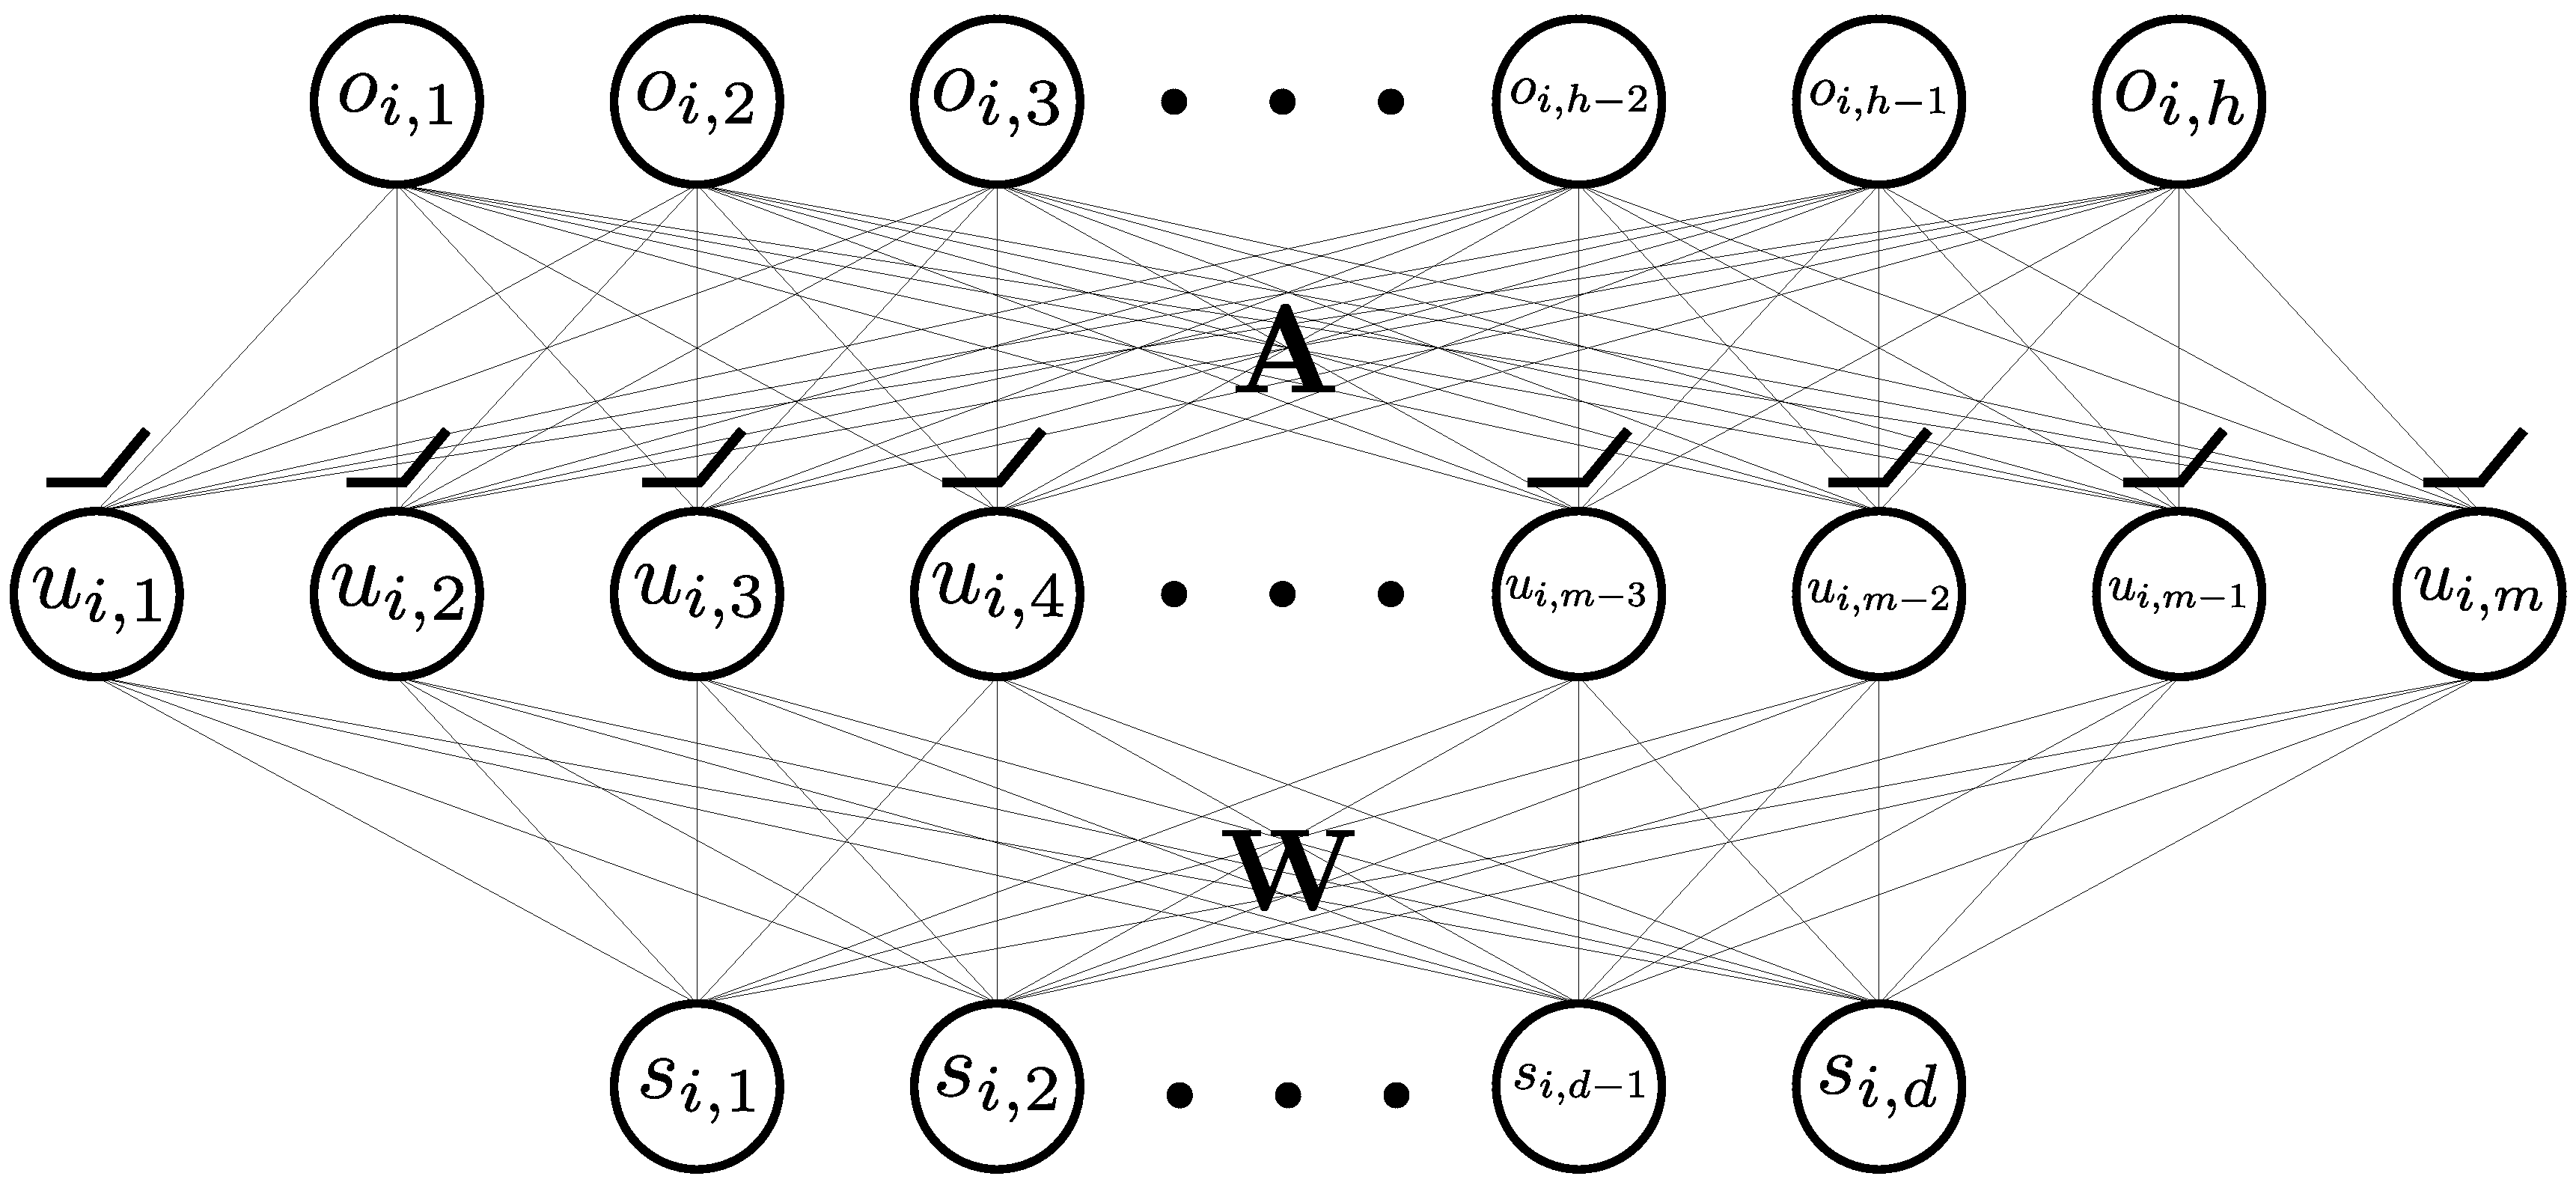
\includegraphics[width=\columnwidth]{nn_value.pdf}}
		\caption{Value neural network.}
		\label{fig:nn_value}
	\end{center}
	\vskip -0.2in
\end{figure}



%We mainly focus on the standard stochastic bandit setting with $n = 1$, i.e., there is only one state $\rvs_i$. At each time step $t$, the agent takes an action $A_t \in [h]$ according to its own strategies, and then it observes a random reward $R_{i, A_t} \in \sR$, where the mean value of $R_{i, A_t}$ is $r_{i, A_t}$. The agent then uses the reward to improve its action selection strategies. After such $T$ time steps, the performance of the agent's strategy is measured by the (expected) regret,
%\begin{equation}
%\label{eq:expected_regret}
%    \sum\limits_{t=0}^{T-1}{{\rvpi_i^*}^\top \rvr_i} - \sE \left[ \sum\limits_{t=0}^{T-1}{  r_{i, A_t}  } \right] = \sum\limits_{t=0}^{T-1}{{\rvpi_i^*}^\top \rvr_i} - \sum\limits_{t=0}^{T-1}{ \sE \left[ r_{i, A_t} \right] },
%\end{equation}
%where the expectation is over the randomness of action selection, if the agent is using some stochastic strategies.


\subsection{NEURAL NETWORK VALUE FUNCTION APPROXIMATION AND POLICY}
\label{subsec:nn_value_policy}
The structure of the value network and the policy network  is a 2-layers fully connected neural network with ReLU activation, as shown in \cref{fig:nn_value} and \cref{fig:nn_policy}, respectively. 
Each neural network takes the state $\rvs \in \sR^d$ as its input, where without loss of generality we assume that $\left\| \rvs \right\|_2 = 1$.
The hidden layer of both networks are denoted by $\rvu   \triangleq W\rvs\in\sR^m$, and the logit output $\rvo \triangleq A\sigma\left( \rvu\right) \in \sR^h$, where $\sigma$ is element-wise ReLU activation function. 
The policy network differs the value network with one additional softmax transform layer in order to output probability distributions, where $\rvpi \triangleq f\left( \rvo \right) = f\left( \rmA \sigma\left( \rmW \rvs \right) \right)$, and $f$ is the softmax function. In the rest of the paper we denote the policy $\rvpi$ by $\rvpi(\rmW)$ to emphasize its parametrization by $\rmW$. 

%Both the value and the policy neural networks take the state feature  $\rvs_i \in \sR^d$ as the input. Then the networks calculate the hidden node value vector by $u_{i,r} \triangleq \rvw_r^\top \rvs_i$, $\forall r \in [m]$. The logit vector is then calculated by $o_{i,k} \triangleq \rva_k^\top \sigma\left( \rvu_i \right)$, $\forall k \in [h]$, where $\sigma$ is element-wise ReLU activation function. The value neural network outputs the logit vector $\rvo_i$. While the policy neural network output probability is the softmax transform of the logit vector, i.e., $\rvpi_i \triangleq f\left( \rvo_i \right) = f\left( \rmA \sigma\left( \rmW \rvs_i \right) \right)$. 

\begin{figure}[t]
\vskip 0.2in
\begin{center}
\centerline{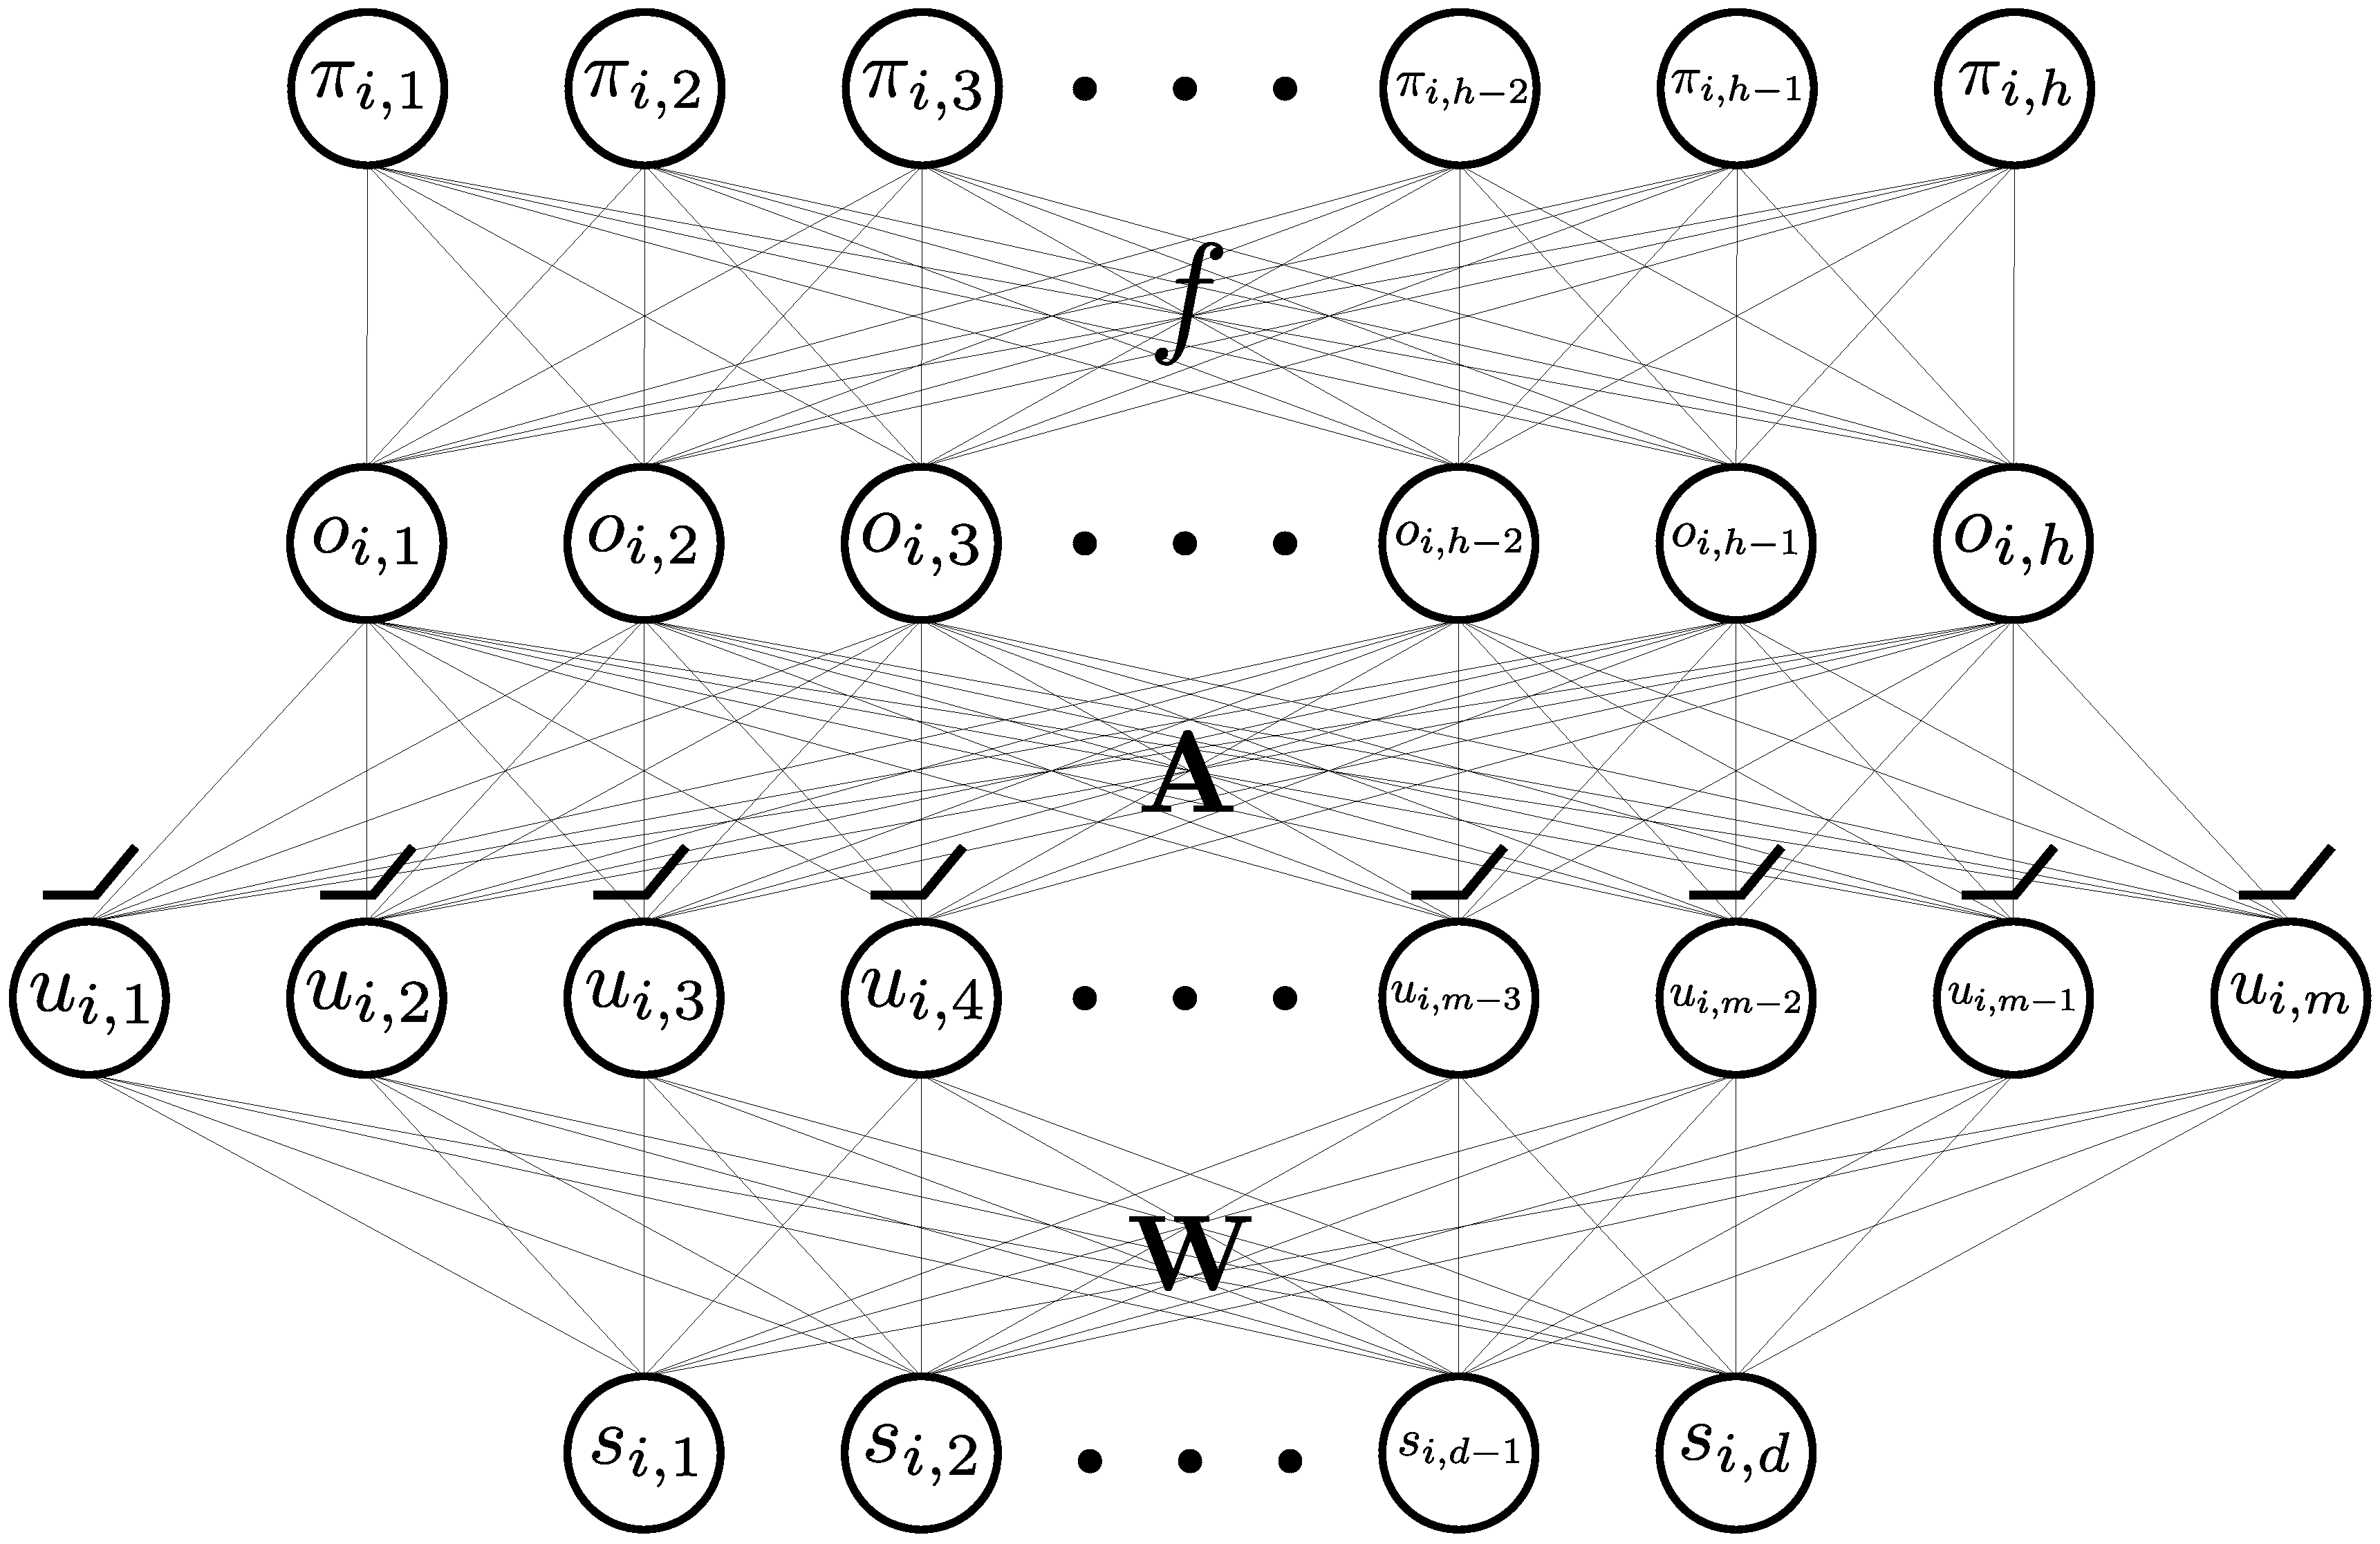
\includegraphics[width=\columnwidth]{nn_policy.pdf}}
\caption{Policy neural network.}
\label{fig:nn_policy}
\end{center}
\vskip -0.2in
\end{figure}

%The policy neural network defines a family of policies $\rvpi_i \left( \rmW \right)$ parameterized by $\rmW \in \sR^{m \times d}$ given any state $\rvs_i$. Let $\rvpi_i = \rvpi_i \left( \rmW \right)$, the expected loss of the policy neural network can be calculated according to \cref{eq:expected_loss}.

\paragraph{Multi-layered neural networks.} We would like to point that our algorithms and results can be easily extended to general value functions and policies parameterized by multi-layered neural networks \citep{allen2018convergenceA,allen2018convergenceB,du2018gradientA}. For the sake of simplicity and conciseness, we focus on two-layers neural networks in the paper.

%Although there is only one state, i.e., $n = 1$, and $i$ can be omitted without ambiguity, we choose to keep the subscript $i$ here to make the generalization from the standard bandit setting to the many state dependent setting smoother, and our algorithms work for general $n > 1$. For simplicity, we assume $\left\| \rvs_{i} \right\|_2 = 1$, $\forall i \in [n]$.

%In the case of $n > 1$, for each state $\rvs_i$, there is a state dependent policy $\rvpi_i$. And the agent's goal is to learn totally $n$ policies using only one neural network. We assume $\left\| \rvs_{i} -  \rvs_{j} \right\|_2 \ge \delta > 0 , \ \forall i \not= j$, i.e., no duplicated data, and $\left\| \rvs_{i} \right\|_2 = 1, \ \forall i \in [n]$.

\subsection{LOGIT LEARNING}
\label{subsec:logit_learning}

Our first proposed algorithm is Logit Learning with $\epsilon$-Greedy Exploration, as shown in \cref{alg:logit_learning_eps_greedy_exploration}. After the random initialization, at each time step $t$, the agent selects the action with the largest logit with probability $1 - \epsilon_t$, and it uniformly randomly select actions with the other probability $\epsilon_t$. After taking action and observing rewards, the agent improves its strategies by minimizing the value loss objective $\frac{1}{2} \left\| \rvo_i\left( \rmW\left(t\right)\right) - \hat{\rvr}_i\left(t\right) \right\|_2^2$, where $\hat{\rvr}_i\left(t\right)$ is the empirical mean reward estimated from sampled rewards up to step $t$. In each iteration, the agent only update its value neural network using one gradient descent, therefore the logit learning is in an online fashion.


\begin{algorithm}[t]
   \caption{Logit Learning with $\epsilon$-Greedy Exploration}
\label{alg:logit_learning_eps_greedy_exploration}
\begin{algorithmic}
   \STATE {\bfseries Input:} State feature $\rvs_i$, learning rate $\eta > 0$.
   \STATE $\rvw_r(0) \sim \gN\left( 0, \sigma^2 \cdot \rmI \right)$, $\forall r \in [m]$.
   \STATE $a_{k, r} \sim \gU\left\{-1, +1\right\}$, $\forall k \in [h]$, $\forall r \in [m]$.
   \STATE $\hat{r}_{i,k}\left(0\right) \gets 0$, $n_{i,k}\left(0\right) \gets 0$, $\forall k \in [h]$.
   \STATE $\hat{\Delta}_{i,k}\left(0\right) \gets \max\limits_{k^\prime}\left\{ \hat{r}_{i,k^\prime}\left(0\right) \right\} - \hat{r}_{i,k}\left(0\right)$, $\forall k \in [h]$.
   \STATE $\tilde{\Delta}_{i,k}\left(0\right) \gets \max\limits_{k^\prime}\left\{ o_{i,k^\prime}\left(0\right) \right\} - o_{i,k}\left(0\right)$, $\forall k \in [h]$.
   \FOR{$t=0$ {\bfseries to} $T-1$}
   \STATE $\xi_t \gets \frac{\log{t}}{t \hat{\Delta}_{i,k}^2\left(0\right)}$, $\epsilon_t \gets \min\left\{ \frac{1}{2 h}, \xi_t \right\}$.
   \STATE $\pi_{i, k}\left(t\right) \gets 1$, for $k = \argmax\limits_{k^\prime \in \left[h\right]}\left\{ o_{i, k^\prime}\left(t\right)\right\}$.
   \STATE $\pi_{i, k}\left(t\right) \gets 0$, $\forall k \not= \argmax\limits_{k^\prime \in \left[h\right]}\left\{ o_{i, k^\prime}\left(t\right)\right\}$.
   \STATE $\tilde{\rvpi}_i\left(t\right) \gets \left( 1 - \epsilon_t \right) \cdot  \rvpi_i\left(t\right) + \epsilon_t \cdot \gU{\left[ h \right]}$.
   \STATE Sample action $A_{t} \sim \tilde{\rvpi}_{i}\left(t\right)\left(\cdot \middle| \rvs_i \right)$.
   \STATE Take action $A_{t}$. Observe reward $R_{i, A_{t}}\left(n_{i, A_{t}}\left(t\right) \right)$.
   \STATE $n_{i, A_{t}}\left(t+1\right) \gets n_{i, A_{t}}\left(t\right) + 1$.
   \STATE $\hat{r}_{i,A_{t}}\left(t+1\right) \gets \frac{n_{i, A_{t}}\left(t\right) \cdot \hat{r}_{i,A_{t}}\left(t\right) + R_{i, A_{t}}\left(n_{i, A_{t}}\left(t\right)\right) }{n_{i, A_{t}}\left(t+1\right)}$.
   \STATE $n_{i, k}\left(t+1\right) \gets n_{i, k}\left(t\right)$, $\forall k \not= A_t$.
   \STATE $\hat{r}_{i,k}\left(t+1\right) \gets \hat{r}_{i,k}\left(t\right)$, $\forall k \not= A_t$.
   \STATE $\rmW(t+1) \leftarrow \rmW(t) - \eta \cdot \frac{d \left\{ \frac{1}{2} \left\| \rvo_i\left( \rmW\left(t\right)\right) - \hat{\rvr}_i\left(t\right) \right\|_2^2 \right\}}{d \rmW(t)}$.
   \ENDFOR
\end{algorithmic}
\end{algorithm}

\subsection{POLICY GRADIENT}
\label{subsec:policy_gradient}

Our second proposed algorithm is based on the widely used policy gradient method. Consider at each step $t$, the agent is using $\rvpi_i\left(\rmW(t)\right)$ as shown in \cref{fig:nn_policy} as its action selection strategy, then the (expected) regret is equivalent to the cumulative expected loss of $\rvpi_i\left(\rmW(t)\right)$, i.e., 
\begin{equation}
\label{eq:vanilla_policy_gradient_expected_regret}
\begin{split}
    &\sum\limits_{t=0}^{T-1}{{\rvpi_i^*}^\top \rvr_i} - \sum\limits_{t=0}^{T-1}{ \expectation\limits_{A_t \sim \rvpi_i\left(\rmW(t)\right)} \left[ r_{i, A_t} \right] } \\
    &= \sum\limits_{t=0}^{T-1}{{\rvpi_i^*}^\top \rvr_i} - \sum\limits_{t=0}^{T-1}{\rvpi_i\left(\rmW(t)\right)^\top \rvr_i},
\end{split}
\end{equation}
by \cref{eq:expected_loss} and \cref{eq:expected_regret}. Using \cref{eq:vanilla_policy_gradient_expected_regret}, at each time step $t$, the agent can use the current NN policy $\rvpi_i\left(\rmW(t)\right)$ to sample an action, and obtain an estimation of the expected loss $\rvpi_i\left(\rmW(t)\right)^\top \rvr_i$. Doing policy gradient updates with respect to the NN weights $\rmW(t)$ will arguably decrease the expected loss, thus reduce the expected regret. 

Unfortunately, the vanilla policy gradient often suffers the ``lack of exploration" problem in practice, i.e., some actions can never be explored thus cannot be learned. Therefore, we propose a two stage algorithm combining policy gradient with uniform exploration as shown in \cref{alg:policy_gradient_uniform_exploration}. After the random initialization, at each step $t$, one of the two cases happens. If $t < T^{\frac{2}{3} + \beta}$, then agent gets into a purely ``exploring phase", without learning the policy neural network, while just collecting empirically estimated rewards. If $t \ge T^{\frac{2}{3} + \beta}$, then the agent starts ``playing and learning". The agent samples and takes actions according to the current neural network policy $\rvpi_{i}\left(\rmW(t)\right)$. In the meanwhile, the agent learns the policy neural network by doing policy gradient updates, with the expected empirically estimated loss calculated from the exploring phase as its objective.

\begin{algorithm}[t]
   \caption{Policy Gradient with Uniform Exploration}
\label{alg:policy_gradient_uniform_exploration}
\begin{algorithmic}
   \STATE {\bfseries Input:} State feature $\rvs_i$, learning rate $\eta > 0$, $\beta > 0$.
   \STATE $\rvw_r(0) \sim \gN\left( 0, \sigma^2 \cdot \rmI \right)$, $\forall r \in [m]$.
   \STATE $a_{k, r} \sim \gU\left\{-1, +1\right\}$, $\forall k \in [h]$, $\forall r \in [m]$.
   \STATE $\hat{r}_{i,k}\left(0\right) \gets 0$, $n_{i,k}\left(0\right) \gets 0$, $\forall k \in [h]$.
   \FOR{$t=0$ {\bfseries to} $T-1$}
   \IF{$t < T^{\frac{2}{3} + \beta}$}
   \STATE (Exploring Phase)
   \STATE Uniformly randomly sample action $A_{t} \in [h]$.
   \STATE $\rmW(t+1) \leftarrow \rmW(t)$.
   \ELSE
   \STATE (Playing-Learning Phase)
   \STATE Sample action $A_{t} \sim \rvpi_{i}\left(\rmW(t)\right)\left(\cdot \middle| \rvs_i \right)$.
   \STATE $\rmW(t+1) \leftarrow \rmW(t) + \eta \cdot \frac{d \rvpi_{i}\left(\rmW(t)\right)^\top \hat{\rvr}_i \left(t\right)}{d \rmW(t)}$.
   \ENDIF
   \STATE Take action $A_{t}$. Observe reward $R_{i, A_{t}}\left(n_{i, A_{t}}\left(t\right) \right)$.
   \STATE $n_{i, A_{t}}\left(t+1\right) \gets n_{i, A_{t}}\left(t\right) + 1$.
   \STATE $\hat{r}_{i,A_{t}}\left(t+1\right) \gets \frac{n_{i, A_{t}}\left(t\right) \cdot \hat{r}_{i,A_{t}}\left(t\right) + R_{i, A_{t}}\left(n_{i, A_{t}}\left(t\right)\right) }{n_{i, A_{t}}\left(t+1\right)}$.
   \STATE $n_{i, k}\left(t+1\right) \gets n_{i, k}\left(t\right)$, $\forall k \not= A_t$.
   \STATE $\hat{r}_{i,k}\left(t+1\right) \gets \hat{r}_{i,k}\left(t\right)$, $\forall k \not= A_t$.
   \ENDFOR
\end{algorithmic}
\end{algorithm}

\paragraph{Initialization of the matrix $\mathbf{A}$.} Note that in \cref{alg:logit_learning_eps_greedy_exploration} and \cref{alg:policy_gradient_uniform_exploration}, after the random initialization $a_{k,r} \sim \gU\left\{-1, +1\right\}$, $a_{k,r}$ is fixed during learning, which is a common assumption in literature \citep{li2018learning,du2018gradientA,du2018gradientB,allen2018convergenceA,allen2018convergenceB}, and it has been empirically verified that there is no impact on the performance of trained neural networks \citep{hoffer2018fix}. Some other initializations like $\rva_k \sim \gN(0, \rmI)$ also work.


\documentclass[10pt]{article}
\usepackage[usenames]{color} %used for font color
\usepackage{amssymb} %maths
\usepackage{amsmath} %maths
\usepackage{amsthm}
\usepackage[utf8]{inputenc} %useful to type directly diacritic characters
\usepackage[capitalize]{cleveref}
\crefname{prop}{Proposition}{Propositions}
\crefname{thm}{Theorem}{Theorems}
\crefname{lem}{Lemma}{Lemmas}

\usepackage{hyperref}

\def\rva{{\mathbf{a}}}
\def\rvo{{\mathbf{o}}}
\def\rvr{{\mathbf{r}}}
\def\rvs{{\mathbf{s}}}
\def\rvu{{\mathbf{u}}}
\def\rvw{{\mathbf{w}}}
\def\rvx{{\mathbf{x}}}
\def\rvg{{\mathbf{g}}}
\def\rvo{{\mathbf{o}}}
\def\rvone{{\mathbf{1}}}
\def\rvzero{{\mathbf{0}}}
\def\rvtilder{{\tilde{\mathbf{r}}}}

\def\rvp{{\mathbf{p}}}

\def\pr{{\text{Pr}}}
\def\r{{\text{R}}}

\def\regret{{\text{Regret}}}

\newtheorem{thm}{Theorem}
\newtheorem{lem}{Lemma}
\newtheorem{defi}{Definition}
\newtheorem{prop}{Proposition}
\newtheorem{remk}{Remark}


\def\rvpi{{\boldsymbol{\pi}}}

\def\rmI{{\mathbf{I}}}
\def\rmW{{\mathbf{W}}}
\def\rmX{{\mathbf{X}}}

\def\sE{{\mathbb{E}}}
\def\sR{{\mathbb{R}}}
\def\sI{{\mathbb{I}}}

\def\gN{{\mathcal{N}}}
\def\gE{{\mathcal{E}}}
\def\gU{{\mathcal{U}}}


\title{Overparameterized Policy Gradient}
\author{}
\date{December 2018}

\DeclareMathOperator*{\argmax}{arg\,max}
\DeclareMathOperator*{\probability}{Pr}

\begin{document}

\maketitle

\section{Notations}

Bold letters refer to vectors, and non-bold letters refer to scalars. For example, $u_{i,r} \in \sR$ is the $r$th component of vector $\rvu_i \in \sR^m$. $n$ is the total number of data points, while $m$ is the total number of nodes in each hidden layer. $h$ is the total number of arms/trajectories of each bandit/starting state.

\begin{itemize}
	\item $\rvs_i \in \sR^d$, $i \in [n]$ is a state/bandit.
	\item $\rvw_r \in \sR^d$, $r \in [m]$ is a weight vector in the first hidden layer.
	\item $u_{i,r} \triangleq \sigma(\rvw_r^\top \rvs_i)$, where $\sigma(\cdot) \triangleq \max\left\{ \cdot, 0 \right\}$ is the ReLU activation function.
	\item $\rva_k \in \sR^m$, $k \in [h]$ is a weight vector in the second layer. $\rva_k \sim \gN(0, \rmI)$.
	\item $o_{i,k} \triangleq \sum\limits_{r=1}^{m}{a_{k,r} \cdot u_{i,r}}$ is the logit of the $k$th arm for state $\rvs_i$.
	\item $\pi_{i,k} \triangleq \frac{\exp\left\{ o_{i,k} \right\}}{\sum\limits_{k^\prime = 1}^{h}{\exp\left\{ o_{i,k^\prime} \right\}}}$ is the  probability for choosing arm $k$ in bandit $i$.
	\item $\rvr_i \in \sR^h$ is the reward vector for bandit $i$.
	\item $\r_i^{\max} \triangleq \max\limits_{k}\left\{ r_{i,k} \right\}$ is the maximum reward of bandit $i$.
	\item The loss/regret $\ell \triangleq \regret(\rvpi) \triangleq \frac{1}{n} \cdot \sum\limits_{i=1}^{n}{ \left( \r_i^{\max} - \rvpi_i^\top \rvr_i \right) }$. Regret minimization is equivalent with maximizing reward $\frac{1}{n} \sum\limits_{i=1}^{n}{\rvpi_i^\top \rvr_i}$.
\end{itemize}

Denote $\rvtilder_{i} \triangleq \r_i^{\max} \cdot \rvone -  \rvr_{i} \ge \rvzero$. The regret at time step $t$ is,
\begin{equation*}
\begin{split}
	\ell(t) \triangleq \regret(\rvpi(t)) &= \frac{1}{n} \cdot \sum\limits_{i=1}^{n}{ \left( \r_i^{\max} - \rvpi_{i}(t)^\top \rvr_i \right) } \\
	&= \frac{1}{n} \cdot \sum\limits_{i=1}^{n}{ \rvpi_{i}(t)^\top \left( \r_i^{\max} \cdot \rvone - \rvr_{i} \right) } \\
	&= \frac{1}{n} \cdot \sum\limits_{i=1}^{n}{ \rvpi_{i}(t)^\top \rvtilder_{i} }.
\end{split}
\end{equation*}

\section{Results}

We analyze the policy gradient method,
\begin{itemize}
	\item Initialize $\rvw_r(0) \sim \gN(0, \sigma^2 \cdot \rmI)$, $\forall r \in [m]$.
	\item Update $\rvw_r(t+1) = \rvw_r(t) - \eta \cdot \frac{d\ell}{d \rvw_r(t)}$.
\end{itemize}

\noindent There are two data assumptions,
\begin{itemize}
	\item $\left\| \rvs_{i} -  \rvs_{j} \right\|_2 \ge \delta > 0 , \ \forall i \not= j$. There is no duplicated data.
	\item $\left\| \rvs_{i} \right\|_2 = 1, \ \forall i \in [n]$.
\end{itemize}

\noindent The main result is,
\begin{thm}
	If $m \ge \frac{n^6}{c^4 \delta^4 \varepsilon^4}$, let $\eta = \frac{1}{m}$, after $t = O\left( \frac{n^2}{ c^2\delta^2\varepsilon^2} \right)$ gradient steps, $\regret\left( \rvpi(t)\right) \le \varepsilon n$.
\end{thm}
\begin{proof}
(Sketch) By \cref{lem:gradient_lower_bound}, unless $\regret\left( \rvpi(t)\right) \le \varepsilon n$, there are $\Omega\left( \frac{m\delta}{n} \right)$ of $\rvw_r(t)$ such that $\left\| \frac{d\tilde{\ell}}{d \rvw_r(t)} \right\|_2 \ge \Omega\left( \frac{c\delta \varepsilon}{n} \right)$. By \cref{lem:gradient_upper_bound}, let $\tau = \frac{\sigma}{n}$, there are $\Omega\left( m \right)$ of $\rvw_r(t)$ such that $\left\| \frac{d\ell}{d \rvw_r(t)} \right\|_2 \ge \Omega\left( \frac{c\delta \varepsilon}{n} \right)$. For $\eta$ small enough, each gradient descent will decrease $l(\rvw)$ by $\Omega\left( \frac{\eta m c^2\delta^2\varepsilon^2}{n^2} \right)$, which means it converges in $O\left( \frac{n^2}{\eta m c^2\delta^2\varepsilon^2} \right)$ steps. Let $\sigma = \left( \frac{1}{\sqrt{m}} \right)$, and $\frac{n^2}{\eta m c^2\delta^2\varepsilon^2} \le \frac{\tau}{\eta} = \frac{\sigma}{\eta n}$, we have $m \ge \frac{n^6}{c^4 \delta^4 \varepsilon^4}$.
\end{proof}

\begin{thm}
    Assume $m \in \tilde{\Theta}\left( \frac{n^{10}}{c^4 \delta^4 \varepsilon^2} \right)$, $\eta \in \Theta\left( \frac{c^2 \delta^2}{16 n^4 h m \left( \log{\left(4m\right)} \right)^2} \right)$, after $t \in O\left( \frac{n^4}{\eta m c^2 \delta^2 \varepsilon} \right)$ iterations, $\rvpi_i\left( \rmW(t) \right)^\top \rvtilder_i \le \varepsilon$, and the regret $\sum\limits_{t=1}^{T}{ \rvpi_i\left( \rmW(t) \right)^\top \rvtilder_i } \le  \frac{8 n^4 \sqrt{h}}{c^2 \delta^2} \cdot \tilde{O}\left( \sqrt{T} \right)$.
\end{thm}
\begin{proof}
    By \cref{lem:gradient_upper_bound}, let $\tau = \frac{\sigma}{n}$, there is $\Omega\left( m \right)$ of $\rvw_r(t)$ such that $\left\| \frac{d\ell}{d \rvw_r(t)} \right\|_2 = \left\| \frac{d\tilde{\ell}}{d \rvw_r(t)} \right\|_2$, $\forall t \in O\left( \frac{\sigma}{\eta n \sqrt{\log{m}}} \right)$. Let $\rmW(t+1) = \rmW(t) - \eta \cdot \frac{d \ell}{d \rmW(t)}$, by \cref{lem:semi_smoothness},
\begin{equation*}
\begin{split}
    \rvpi_i\left( \rmW(t+1) \right)^\top \rvtilder_i &\le \rvpi_i\left( \rmW(t) \right)^\top \rvtilder_i - \eta \cdot \left\| \frac{d \ell}{d \rmW(t)} \right\|_F^2 \\
    &\qquad + 4 \sqrt{m \log{\left(4m\right)}} \cdot \rvpi_i\left( \rmW \right)^\top \rvtilder_i \cdot \eta \cdot \left\| \frac{d \ell}{d \rmW(t)} \right\|_F \\
    &\qquad + 4 h m \log{\left(4m\right)} \cdot \eta^2 \left\| \frac{d \ell}{d \rmW(t)} \right\|_F^2 \\
    &\le \rvpi_i\left( \rmW(t) \right)^\top \rvtilder_i - \eta \cdot \sum\limits_{r=1}^{m}{ \left\| \frac{d\ell}{d \rvw_r(t)} \right\|_2^2 } \\
    &\qquad + 4 \sqrt{m \log{\left(4m\right)}} \cdot \rvpi_i\left( \rmW \right)^\top \rvtilder_i \cdot \eta \cdot \sum\limits_{r=1}^{m}{ \left\| \frac{d\ell}{d \rvw_r(t)} \right\|_2 } \\
    &\qquad + 4 h m \log{\left(4m\right)} \cdot \eta^2 \cdot \sum\limits_{r=1}^{m}{ \left\| \frac{d\ell}{d \rvw_r(t)} \right\|_2^2 } \\
    \le \rvpi_i\left( \rmW(t) \right)^\top \rvtilder_i - \left( \rvpi_i\left( \rmW(t) \right)^\top \rvtilder_i \right)^2 &\cdot \left[ \frac{\eta m c^2 \delta^2}{n^4} - 8 \eta m \sqrt{m} \log{\left(4m\right)} - 16 \eta^2 h m^2 \left( \log{\left(4m\right)} \right)^2 \right] \\
    &= \rvpi_i\left( \rmW(t) \right)^\top \rvtilder_i - \left( \rvpi_i\left( \rmW(t) \right)^\top \rvtilder_i \right)^2 \cdot \Omega\left( \frac{\eta m c^2 \delta^2}{n^4} \right).
\end{split}
\end{equation*}
Divide the above by $\left( \rvpi_i\left( \rmW(t+1) \right)^\top \rvtilder_i\right) \cdot \left( \rvpi_i\left( \rmW(t) \right)^\top \rvtilder_i \right)$,
\begin{equation*}
\begin{split}
    \frac{1}{\rvpi_i\left( \rmW(t+1) \right)^\top \rvtilder_i} - \frac{1}{\rvpi_i\left( \rmW(t) \right)^\top \rvtilder_i} \ge \frac{\rvpi_i\left( \rmW(t) \right)^\top \rvtilder_i}{\rvpi_i\left( \rmW(t+1) \right)^\top \rvtilder_i} \cdot \Omega\left( \frac{\eta m c^2 \delta^2}{n^4} \right) \ge \Omega\left( \frac{\eta m c^2 \delta^2}{n^4} \right).
\end{split}
\end{equation*}
Sum up the inequality from $0$ to $t$,
\begin{equation*}
\begin{split}
    \frac{1}{\rvpi_i\left( \rmW(t) \right)^\top \rvtilder_i} \ge \Omega\left( \frac{\eta m c^2 \delta^2}{n^4} \right) \cdot t + \frac{1}{\rvpi_i\left( \rmW(0) \right)^\top \rvtilder_i} \ge \Omega\left( \frac{\eta m c^2 \delta^2}{n^4} \right) \cdot t.
\end{split}
\end{equation*}
Therefore after $t \in O\left( \frac{n^4}{\eta m c^2 \delta^2 \varepsilon} \right)$ iterations, $\rvpi_i\left( \rmW(t) \right)^\top \rvtilder_i \le \varepsilon$. Let $\frac{n^4}{\eta m c^2 \delta^2 \varepsilon} \le \frac{\sigma}{n \eta \sqrt{\log{m}}} = \frac{1}{n \eta \sqrt{m \log{m}}}$, we have $m \ge \frac{n^{10}}{c^4 \delta^4 \varepsilon^2}\log{\left( \frac{n^{10}}{c^4 \delta^4 \varepsilon^2} \right)}$. Moreover,
\begin{equation*}
\begin{split}
    \sum\limits_{t=1}^{T}{ \rvpi_i\left( \rmW(t) \right)^\top \rvtilder_i } &\le t \cdot 1 + \left(T - t\right) \cdot \varepsilon \\
    &\le t + \frac{n^4}{\eta m c^2 \delta^2} \cdot \frac{T}{t} \\
    &\le \frac{2 n^2}{c \delta} \cdot \frac{1}{\sqrt{\eta m}} \cdot \sqrt{T} \\
    &\le \frac{8 n^4 \sqrt{h}}{c^2 \delta^2} \cdot \log{\left(4m\right)} \cdot \sqrt{T} \\
    &\le \frac{8 n^4 \sqrt{h}}{c^2 \delta^2} \cdot \tilde{O}\left(\sqrt{T}\right). \qedhere
\end{split}
\end{equation*}
\end{proof}

\subsection{Policy Gradient}

\subsubsection{One Form}

The gradient with respect to $\rvw_r(t)$ is,
\begin{equation}
\label{eq:gradient_form_one}
\begin{split}
	\frac{d\ell}{d \rvw_r(t)} &= \frac{1}{n} \cdot \sum\limits_{i=1}^{n}{ \sum\limits_{k=1}^{h}\left[ \tilde{r}_{i,k} \cdot \frac{d \pi_{i,k}(t)}{d \rvw_r(t)} \right] } \\
	&= \frac{1}{n} \cdot \sum\limits_{i=1}^{n}{ \sum\limits_{k=1}^{h}\left[ \tilde{r}_{i,k} \cdot \frac{d}{d \rvw_r(t)} \left\{ \frac{\exp\left\{ o_{i,k}(t) \right\}}{\sum\limits_{k^\prime = 1}^{h}{\exp\left\{ o_{i,k^\prime}(t) \right\}}} \right\} \right] } \\
	&= \frac{1}{n} \cdot \sum\limits_{i=1}^{n}{ \sum\limits_{k=1}^{h}\left[ \tilde{r}_{i,k} \cdot \frac{ \exp\left\{ o_{i,k}(t) \right\} \cdot a_{k,r} \cdot \rvs_i \cdot \sI\left\{ \rvw_r(t)^\top \rvs_i > 0 \right\} \cdot \left( \sum\limits_{k^\prime = 1}^{h}{\exp\left\{ o_{i,k^\prime}(t) \right\}} \right) }{ \left( \sum\limits_{k^\prime = 1}^{h}{\exp\left\{ o_{i,k^\prime}(t) \right\}} \right)^2 } \right] } \\
	&\qquad - \frac{1}{n} \cdot \sum\limits_{i=1}^{n}{ \sum\limits_{k=1}^{h}\left[ \tilde{r}_{i,k} \cdot \frac{ \exp\left\{ o_{i,k}(t) \right\} \cdot \sum\limits_{k^\prime = 1}^{h}{\exp\left\{ o_{i,k^\prime}(t) \right\}} \cdot a_{k^\prime,r} \cdot \rvs_i \cdot \sI\left\{ \rvw_r(t)^\top \rvs_i > 0 \right\} }{ \left( \sum\limits_{k^\prime = 1}^{h}{\exp\left\{ o_{i,k^\prime}(t) \right\}} \right)^2 } \right] } \\
	&= \frac{1}{n} \cdot \sum\limits_{i=1}^{n}{ \sum\limits_{k=1}^{h}{ \left[ \tilde{r}_{i,k} \cdot \pi_{i,k}(t) \cdot \left( \sum\limits_{k^\prime = 1}^{h}{ a_{k,r} \cdot \pi_{i,k^\prime}(t) } - \sum\limits_{k^\prime = 1}^{h}{ a_{k^\prime,r} \cdot \pi_{i,k^\prime}(t) } \right) \cdot \sI\left\{ \rvw_r(t)^\top \rvs_i > 0 \right\} \cdot \rvs_i \right] } } \\
	&= \frac{1}{n} \cdot \sum\limits_{i=1}^{n}{ \sum\limits_{k=1}^{h}{ \left[ \tilde{r}_{i,k} \cdot \pi_{i,k}(t) \cdot \left( \sum\limits_{k^\prime \not= k}^{h}{ \pi_{i,k^\prime}(t) \cdot \left( a_{k,r} - a_{k^\prime,r} \right)  } \right) \cdot \sI\left\{ \rvw_r(t)^\top \rvs_i > 0 \right\} \cdot \rvs_i \right] } } \\
	&= \frac{1}{n} \cdot \sum\limits_{i=1}^{n}{ \sum\limits_{k=1}^{h}{ \left[ \tilde{r}_{i,k} \cdot \pi_{i,k}(t) \cdot \left( \sum\limits_{k^\prime = 1}^{h}{ a_{k^\prime,r}  \cdot v_{k^\prime,k,i}(t) } \right) \cdot \sI\left\{ \rvw_r(t)^\top \rvs_i > 0 \right\} \cdot \rvs_i \right] } },
\end{split}
\end{equation}
where $v_{k^\prime,k,i}(t)$ is defined as,
\begin{equation*}
	v_{k^\prime,k,i}(t) = \begin{cases}
    1 - \pi_{i,k^\prime}(t), & \text{if $k^\prime = k$}, \\
    - \pi_{i,k^\prime}(t), & \text{otherwise}.
  \end{cases}
\end{equation*}

\subsubsection{Another Form}

First note that, $\forall k \in [h]$,
\begin{equation*}
\begin{split}
    \frac{d \rvpi_i(t)^\top \rvtilder_i}{d o_{i,k}(t)} &= \sum\limits_{k^\prime = 1}^{h}{ \tilde{r}_{i, k^\prime} \cdot \frac{d \pi_{i,k^\prime}(t) }{d o_{i,k}(t)}} \\
    &= \sum\limits_{k^\prime = 1}^{h}{ \tilde{r}_{i, k^\prime} \cdot \frac{d }{d o_{i,k}(t)}} \left\{ \frac{\exp\left\{ o_{i,k^\prime}(t) \right\}}{\sum\limits_{k^\prime = 1}^{h}{\exp\left\{ o_{i,k^\prime}(t) \right\}}} \right\} \\
    &= \tilde{r}_{i, k} \cdot \frac{ \exp\left\{ o_{i,k}(t) \right\} \cdot \left( \sum\limits_{k^\prime = 1}^{h}{\exp\left\{ o_{i,k^\prime}(t) \right\}} \right) - \exp\left\{ o_{i,k}(t) \right\} \cdot \exp\left\{ o_{i,k}(t) \right\} }{ \left( \sum\limits_{k^\prime = 1}^{h}{\exp\left\{ o_{i,k^\prime}(t) \right\}} \right)^2 } \\
    &\quad - \sum\limits_{k^\prime \not= k}{ \tilde{r}_{i, k^\prime} \cdot \frac{\exp\left\{ o_{i,k^\prime}(t) \right\} \cdot \exp\left\{ o_{i,k}(t) \right\} }{ \left( \sum\limits_{k^\prime = 1}^{h}{\exp\left\{ o_{i,k^\prime}(t) \right\}} \right)^2 }} \\
    &= \tilde{r}_{i, k} \cdot \left( \pi_{i,k}(t) - \pi_{i,k}(t)^2 \right) - \sum\limits_{k^\prime \not= k}{ \tilde{r}_{i, k^\prime} \cdot \pi_{i,k^\prime}(t) \cdot \pi_{i,k}(t) } \\
    &= \pi_{i,k}(t) \cdot \left( \tilde{r}_{i, k} - \rvpi_i(t)^\top \rvtilder_i \right).
\end{split}
\end{equation*}

\noindent For the vector derivative, we have,
\begin{equation*}
\begin{split}
    \frac{d \rvpi_i(t)^\top \rvtilder_i}{d \rvo_{i}(t)} &= \left( \Delta\left( \rvpi_i(t) \right) - \rvpi_i(t) \rvpi_i(t)^\top \right) \rvtilder_i .
\end{split}
\end{equation*}

\noindent Also note that, $\forall r \in [m]$, $\forall k \in [h]$,
\begin{equation*}
\begin{split}
    \frac{d o_{i,k}(t)}{d \rvw_r(t)} &= a_{k,r} \cdot \frac{d u_{i,r}(t)}{d \rvw_r(t)} \\
    &= a_{k,r} \cdot \sI\left\{ \rvw_r(t)^\top \rvs_i > 0 \right\} \cdot \rvs_i.
\end{split}
\end{equation*}

\noindent Then the gradient with respect to $\rvw_r(t)$ is,
\begin{equation}
\label{eq:gradient_form_two}
\begin{split}
    \frac{d\ell}{d \rvw_r(t)} &= \frac{1}{n} \cdot \sum\limits_{i=1}^{n}{ \frac{d \rvpi_i(t)^\top \rvtilder_i}{d \rvw_r(t)} } \\
    &= \frac{1}{n} \cdot \sum\limits_{i=1}^{n}{ \sum\limits_{k=1}^{h}{ \frac{d \rvpi_i(t)^\top \rvtilder_i}{d o_{i,k}(t)}\cdot \frac{d o_{i,k}(t)}{d \rvw_r(t)} } } \\
    &= \frac{1}{n} \cdot \sum\limits_{i=1}^{n}{ \sum\limits_{k=1}^{h}{ \left[ \pi_{i,k}(t) \cdot \left( \tilde{r}_{i, k} - \rvpi_i(t)^\top \rvtilder_i \right) \cdot a_{k,r} \cdot \sI\left\{ \rvw_r(t)^\top \rvs_i > 0 \right\} \cdot \rvs_i  \right] }  } \\
    &= \frac{1}{n} \cdot \sum\limits_{i=1}^{n}{ \left[ \rvtilder_i^\top \left( \Delta\left( \rvpi_i(t) \right) - \rvpi_i(t) \rvpi_i(t)^\top \right) \rva_{\cdot, r} \cdot \sI\left\{ \rvw_r(t)^\top \rvs_i > 0 \right\} \cdot \rvs_i  \right] },
\end{split}
\end{equation}
where $\rva_{\cdot, r} \in \sR^h$ refers to $\rva_{\cdot, r} \triangleq \left( a_{1,r}, a_{2,r}, \dots, a_{h,r} \right)^\top$. It is easy to check that \cref{eq:gradient_form_one} and \cref{eq:gradient_form_two} are equivalent.

\subsection{Gradient Norm Upper Bound}

\begin{lem}
\label{lem:gradient_upper_bound}
	Define the pseudo gradient as,
\begin{equation*}
	\frac{d \tilde{\ell}}{d \rvw_r(t)} \triangleq \frac{1}{n} \cdot \sum\limits_{i=1}^{n}{ \sum\limits_{k=1}^{h}{ \left[ \tilde{r}_{i,k} \cdot \pi_{i,k}(t) \cdot \left( \sum\limits_{k^\prime = 1}^{h}{ a_{k^\prime,r}  \cdot v_{k^\prime,k,i}(t) } \right) \cdot \sI\left\{ \rvw_r(0)^\top \rvs_i > 0 \right\} \cdot \rvs_i \right] } }.
\end{equation*}
	For any $\tau > 0$, with probability at least $\frac{1}{2} \cdot \left( 1 - \frac{\sqrt{2}n\tau}{\sqrt{\pi}\sigma} \right)$, $\forall t \in O\left(\frac{\tau}{\eta  \sqrt{\log{m}}}\right)$,
\begin{equation}
	\frac{d\ell}{d \rvw_r(t)} = \frac{d \tilde{\ell}}{d \rvw_r(t)}.
\end{equation}
\end{lem}
\begin{proof}
The policy gradient is,
\begin{equation*}
	\frac{d\ell}{d \rvw_r(t)} = \frac{1}{n} \cdot \sum\limits_{i=1}^{n}{ \sum\limits_{k=1}^{h}{ \left[ \tilde{r}_{i,k} \cdot \pi_{i,k}(t) \cdot \left( \sum\limits_{k^\prime \not= k}^{h}{ \pi_{i,k^\prime}(t) \cdot \left( a_{k,r} - a_{k^\prime,r} \right)  } \right) \cdot \sI\left\{ \rvw_r(t)^\top \rvs_i > 0 \right\} \cdot \rvs_i \right] } }.
\end{equation*}
Since $a_{k,r}, a_{k^\prime,r} \sim \gN(0, 1)$, we have $a_{k,r} - a_{k^\prime,r} \sim \gN(0, 2)$, therefore $\left| a_{k,r} - a_{k^\prime,r} \right| \le 2 \sqrt{\log{\left(4m\right)}}$, $\forall k \in [m]$, with  probability at least $\frac{1}{2} $. Then we have,
\begin{equation*}
\begin{split}
	\left\| \frac{d\ell}{d \rvw_r(t)} \right\|_2 &\le \frac{1}{n} \cdot \sum\limits_{i=1}^{n}{ \sum\limits_{k=1}^{h}{ \left| \tilde{r}_{i,k} \cdot \pi_{i,k}(t) \cdot \sum\limits_{k^\prime \not= k}^{h}{ \pi_{i,k^\prime}(t) \cdot \left( a_{k,r} - a_{k^\prime,r} \right)  } \cdot \sI\left\{ \rvw_r(t)^\top \rvs_i > 0 \right\} \right| \cdot \left\| \rvs_i \right\|_2 }} \\
	&\le \frac{2 \sqrt{\log{\left(4m\right)}}}{n} \cdot \sum\limits_{i=1}^{n}{ \sum\limits_{k=1}^{h}{ \tilde{r}_{i,k} \cdot \pi_{i,k}(t) \sum\limits_{k^\prime \not= k}^{h}{ \pi_{i,k^\prime}(t)  } \cdot \left\| \rvs_i \right\|_2  }} \\
	&\le \frac{2 \sqrt{\log{\left(4m\right)}}}{n} \cdot \sum\limits_{i=1}^{n}{ \rvpi_{i}(t)^\top \rvtilder_i } \\
	&= 2 \sqrt{\log{\left(4m\right)}} \cdot \regret(\rvpi(t)).
\end{split}
\end{equation*}
Denote $\regret_{\max} \triangleq \max\limits_{s \ge 0}\left\{\regret\left( \rvpi(s) \right)\right\}$. $\rvw_r(t)$ will be closed to $\rvw_r(0)$,
\begin{equation*}
\begin{split}
	\left\| \rvw_r(t) - \rvw_r(0) \right\|_2 &\le \eta \cdot \sum\limits_{s=0}^{t-1}{\left\| \frac{d\ell}{d \rvw_r(s)} \right\|_2} \\
	&\le \eta \cdot 2 \sqrt{\log{\left(4m\right)}} \cdot \sum\limits_{s=0}^{t-1}{ \regret(\rvpi(s)) } \\
	&\le \eta \cdot 2 \sqrt{\log{\left(4m\right)}} \cdot \regret_{\max} \cdot t .
\end{split}
\end{equation*}
Since $\rvw_r(0)^\top \rvs_i \sim \gN(0, \sigma^2)$, $\pr\left(\left| \rvw_r(0)^\top \rvs_i \right| \le \tau\right) \le  \frac{\sqrt{2}\tau}{\sqrt{\pi}\sigma}$,
\begin{equation*}
\begin{split}
	\pr\left(\forall i \in [n], \left| \rvw_r(0)^\top \rvs_i \right| > \tau\right) &= 1 - \pr\left(\exists i \in [n], \left| \rvw_r(0)^\top \rvs_i \right| \le \tau\right) \\
	&\ge 1 - \sum\limits_{i=1}^{n}{ \pr\left(\left| \rvw_r(0)^\top \rvs_i \right| \le \tau\right) } \\
	&\ge 1 - \frac{\sqrt{2}n\tau}{\sqrt{\pi}\sigma},
\end{split}
\end{equation*}
Condition on the above event happens, let $t \le \frac{\tau}{ \eta \cdot 2 \sqrt{\log{\left(4m\right)}} \cdot \regret_{\max} }$, $\forall i \in [n]$,
\begin{equation*}
\begin{split}
	\left| \left( \rvw_r(t) - \rvw_r(0) \right)^\top \rvs_i \right| &\le \left\| \rvw_r(t) - \rvw_r(0) \right\|_2 \cdot \left\| \rvs_i \right\|_2 \\
	&\le \eta \cdot 2 \sqrt{\log{\left(4m\right)}} \cdot \regret_{\max} \cdot t \\
	&\le \tau < \left| \rvw_r(0)^\top \rvs_i \right|,
\end{split}
\end{equation*}
which implies if $\left| \rvw_r(0)^\top \rvs_i \right| > \tau$, $\forall i \in [n]$, then,
\begin{equation*}
\begin{split}
	\sI\left\{ \rvw_r(t)^\top \rvs_i > 0 \right\} &= \sI\left\{ \rvw_r(0)^\top \rvs_i  + \left( \rvw_r(t) - \rvw_r(0) \right)^\top \rvs_i > 0 \right\} \\
	&= \sI\left\{ \rvw_r(0)^\top \rvs_i > 0 \right\}. \qedhere
\end{split}
\end{equation*}
\end{proof}

\subsection{Gradient Norm Lower Bound}

\begin{lem}
\label{lem:gradient_lower_bound}
	Denote $i^*(t) \triangleq \argmax\limits_{i \in [n]}\left\{\regret(\rvpi_i(t))\right\}$, $k^*(t) \triangleq \argmax\limits_{k \in [h]}\left\{ r_{i^*(t),k} \right\} = \r_{i^*(t)}^{\max}$, i.e., the optimal arm of state $i^*(t)$. If $\pi_{i^*(t), k^*(t)}(t) > c > 0$, where $c$ is a constant, then with probability $\Omega\left( \frac{\delta}{n} \right)$,
\begin{equation*}
\begin{split}
	\left\| \frac{d\tilde{\ell}}{d \rvw_r(t)} \right\|_2 \ge \Omega\left( \frac{c\delta}{n^2} \right) \cdot \regret\left( \rvpi_{i^*(t)}(t) \right) \ge \Omega\left( \frac{c\delta}{n^2} \right) \cdot \regret\left( \rvpi(t) \right).
\end{split}
\end{equation*}
\end{lem}
\begin{proof}
	 For conciseness, we denote $i^*(t)$ as $i^*$, and $k^*(t)$ as $k^*$. Rewrite $\frac{d\tilde{\ell}}{d \rvw_r(t)} = \sum\limits_{k^
	\prime=1}^{h}{ a_{k^\prime,r} \cdot \rvp_{k^\prime, r} }$, where $\rvp_{k^\prime, r} \in \sR^d$ is defined as, 
\begin{equation*}
	\rvp_{k^\prime, r} \triangleq \frac{1}{n} \cdot \sum\limits_{i=1}^{n}{ \sum\limits_{k=1}^{h}{ \left[ \tilde{r}_{i,k} \cdot \pi_{i,k}(t) \cdot v_{k^\prime,k,i}(t) \cdot \sI\left\{ \rvw_r(0)^\top \rvs_i > 0 \right\} \cdot \rvs_i \right] } }.
\end{equation*}
By the randomness of $a_{k^\prime,r}$,
\begin{equation}
\label{eq:gradient_p_lowerbound}
\begin{split}
	\left\| \frac{d\tilde{\ell}}{d \rvw_r(t)} \right\|_2 &\ge \left| a_{k^*,r} \right| \cdot \left\| \rvp_{k^*, r}\right\|_2 \\
	&\ge \left\| \rvp_{k^*, r}\right\|_2,
\end{split}
\end{equation}
with probability at least $\frac{1}{2} - \frac{1}{\sqrt{2\pi}}$. We can decompose $\rvw_r(0)$ as,
\begin{equation}
\label{eq:decompose_w}
\begin{split}
	\rvw_r(0) &= \rvw_r^\prime(0) + \rvw_r^{\prime\prime}(0) \\
	&\triangleq \left( \rmI - \rvs_{i^*}\rvs_{i^*}^\top \right) \rvw_r(0) +  \rvs_{i^*}\rvs_{i^*}^\top \rvw_r(0),
\end{split}
\end{equation}
where $\rvw_r^\prime(0) \perp \rvw_r^{\prime\prime}(0)$. Define $h_{k^*,r}$ as follows,
\begin{equation*}
\begin{split}
	h_{k^*,r} &\triangleq \rvw_r(0)^\top \rvp_{k^*, r} \\
	&= \frac{1}{n} \cdot \sum\limits_{i=1}^{n}{ \sum\limits_{k=1}^{h}{ \left[ \tilde{r}_{i,k} \cdot \pi_{i,k}(t) \cdot v_{k^*,k,i}(t) \cdot \sigma( \rvw_r(0)^\top \rvs_i ) \right] } }.
\end{split}
\end{equation*}
And decompose $h_{k^*,r}$ into two parts, i.e., $i^*$ and $[n] \setminus \left\{ i^* \right\}$,
\begin{equation}
\label{eq:decompose_h}
\begin{split}
	h_{k^*,r} &= \frac{1}{n} \cdot \sum\limits_{k=1}^{h}{ \left[ \tilde{r}_{i^*,k} \cdot \pi_{i^*,k}(t) \cdot v_{k^*,k,i^*}(t) \cdot \sigma( \rvw_r(0)^\top \rvs_i^* ) \right] } \\
	&+ \frac{1}{n} \cdot \sum\limits_{i \not= i^*}{\sum\limits_{k=1}^{h}{ \left[ \tilde{r}_{i,k} \cdot \pi_{i,k}(t) \cdot v_{k^*,k,i}(t) \cdot \sigma( \rvw_r(0)^\top \rvs_i ) \right] } }.
\end{split}
\end{equation}
Consider the following events,
\begin{equation*}
\begin{split}
	\gE_1 &: \left| \rvw_r(0)^\top \rvs_{i^*} \right| \le \tau, \ \text{given } \tau \in \left( 0, \sigma \right], \\
	\gE_2 &: \left| \rvw_r^\prime(0)^\top \rvs_i \right| > \tau, \ \forall i \not= i^*.
\end{split}
\end{equation*}
For $\gE_1$, note $\rvw_r(0)^\top \rvs_{i^*} \sim \gN(0, \sigma^2)$,
\begin{equation*}
\begin{split}
	\pr\left(\gE_1\right) &= \frac{1}{\sqrt{2\pi}\sigma} \int_{-\tau}^{\tau}{\exp\left\{ - \frac{x^2}{2\sigma^2} \right\} dx} \\
	&\ge \frac{1}{\sqrt{2\pi}\sigma} \int_{-\tau}^{\tau}{ \left( 1  - \frac{x^2}{2\sigma^2} \right) dx} \\
	&= \frac{\sqrt{2}}{\sqrt{\pi}\sigma} \cdot \left( \tau - \frac{\tau^3}{6\sigma^2}\right) \\
	&\ge \frac{5\sqrt{2}}{6\sqrt{\pi}} \cdot \frac{\tau}{\sigma} \in \Omega\left( \frac{\tau}{\sigma} \right).
\end{split}
\end{equation*}
For $\gE_2$, according to \cref{eq:decompose_w}, $\rvw_r^\prime(0)^\top \rvs_i \sim \gN\left(0, \left(1 - \left(\rvs_{i^*}^\top \rvs_{i} \right)^2 \right)\sigma^2 \right)$, $\forall i \not= i^*$, and $\rvw_r^\prime(0)^\top \rvs_i$ is independent with $\rvw_r^{\prime\prime}(0)^\top \rvs_{i}$.
\begin{equation*}
\begin{split}
	\pr\left(\gE_2\right) &= 1 - \pr\left( \exists i \not= i^*, \ \left| \rvw_r^\prime(0)^\top \rvs_i \right| \le \tau \right) \\
	&\ge 1 - \sum\limits_{i \not= i^*}{ \pr\left(\left| \rvw_r^\prime(0)^\top \rvs_i \right| \le \tau \right) } \\
	&\ge 1 - \frac{\sqrt{2}n\tau}{\sqrt{\pi\left( 1 - \left(\rvs_{i^*}^\top \rvs_{i} \right)^2 \right) }\sigma} \\
	&\ge 1 - \frac{2n\tau}{\sqrt{\pi}\delta\sigma} \quad \left( \left\| \rvs_{i} -  \rvs_{j} \right\|_2 \ge \delta, \ \forall i \not= j \right).
\end{split}
\end{equation*}
Let $\tau = \frac{\delta\sigma}{2n}$, then $\pr\left(\gE_2\right) \ge 1 - \frac{1}{\sqrt{\pi}}$. Therefore, $\pr\left( \gE_1 \land \gE_2 \right) \in \Omega\left( \frac{\tau}{\sigma} \right)$. Now condition on $\gE_1 \land \gE_2$ happens, we have, $\forall i \not= i^*$,
\begin{equation*}
\begin{split}
	\sI\left\{ \rvw_r(0)^\top \rvs_i > 0 \right\} &= \sI\left\{ \rvw_r^\prime(0)^\top \rvs_i + \rvw_r^{\prime\prime}(0)^\top \rvs_{i} > 0 \right\} \\
	&= \sI\left\{ \rvw_r^\prime(0)^\top \rvs_i > 0 \right\},
\end{split}
\end{equation*}
since $\left| \rvw_r^{\prime\prime}(0)^\top \rvs_{i} \right| = \left| \rvw_r(0)^\top \rvs_{i^*} \rvs_{i^*}^\top \rvs_{i} \right| \le \left| \rvw_r(0)^\top \rvs_{i^*} \right| \le \tau < \left| \rvw_r^\prime(0)^\top \rvs_i  \right|$. Fix $\rvw_r^\prime(0)^\top \rvs_i$, and randomly generate $x \triangleq \rvw_r(0)^\top \rvs_{i^*}$, rewrite \cref{eq:decompose_h},
\begin{equation}
\label{eq:h_alpha}
\begin{split}
	h_{k^*,r} &= \frac{1}{n} \cdot \sum\limits_{k=1}^{h}{ \left[ \tilde{r}_{i^*,k} \cdot \pi_{i^*,k}(t) \cdot v_{k^*,k,i^*}(t) \cdot \sigma(x) \right] } \\
	&+ \frac{1}{n} \cdot \sum\limits_{i \not= i^*}{\sum\limits_{k=1}^{h}{ \left[ \tilde{r}_{i,k} \cdot \pi_{i,k}(t) \cdot v_{k^*,k,i}(t) \cdot ( x \cdot \rvs_{i^*}^\top \rvs_{i} + \rvw_r^\prime(0)^\top \rvs_i ) \cdot \sI\left\{ \rvw_r^\prime(0)^\top \rvs_i > 0 \right\}  \right] } }.
\end{split}
\end{equation}
Note the first part of $h_{k^*,r}$ is a convex function of $x$, and the second part is linear. For the first term in \cref{eq:h_alpha}, we have,
\begin{equation*}
\begin{split}
	\sum\limits_{k=1}^{h}{ \left[ \tilde{r}_{i^*,k} \cdot \pi_{i^*,k}(t) \cdot v_{k^*,k,i^*}(t) \right] } &= \underbrace{\tilde{r}_{i^*,k^*} \cdot \pi_{i^*,k^*}(t) \cdot v_{k^*,k^*,i^*}(t)}_{\tilde{r}_{i^*,k^*} = \r_{i^*}^{\max} -  r_{i^*,k^*} = 0} + \sum\limits_{k\not=k^*}{ \left[ \tilde{r}_{i^*,k} \cdot \pi_{i^*,k}(t) \cdot v_{k^*,k,i^*}(t) \right] } \\
	&= - \pi_{i^*,k^*}(t) \cdot \sum\limits_{k\not=k^*}{ \left[ \tilde{r}_{i^*,k} \cdot \pi_{i^*,k}(t) \right] } \\
	&= - \pi_{i^*,k^*}(t) \cdot \sum\limits_{k=1}^{h}{ \left[ \tilde{r}_{i^*,k} \cdot \pi_{i^*,k}(t) \right] } \\
	&= - \pi_{i^*,k^*}(t) \cdot \regret(\rvpi_{i^*}(t)).
\end{split}
\end{equation*}
By assumption, if $\pi_{i^*,k^*}(t) > c > 0$, then ,
\begin{equation*}
\begin{split}
	\left| \partial{h_{k^*,r}}_{\max}{(0)} - \partial{h_{k^*,r}}_{\min}{(0)} \right| &= \frac{1}{n} \cdot \left| \sum\limits_{k=1}^{h}{ \left[ \tilde{r}_{i^*,k} \cdot \pi_{i^*,k}(t) \cdot v_{k^*,k,i^*}(t) \right] } \right| \\
	&= \frac{1}{n} \cdot \pi_{i^*,k^*}(t) \cdot \regret(\rvpi_{i^*}(t)) \\
	&\ge \frac{c}{n} \cdot \regret(\rvpi(t)).
\end{split}
\end{equation*}
where $\partial{h_{k^*,r}}_{\max}{(0)} = \max\left\{ \partial{h_{k^*,r}}{(0)} \right\}$, $\partial{h_{k^*,r}}_{\min}{(0)} = \min\left\{ \partial{h_{k^*,r}}{(0)} \right\}$ are the maximum and minimum of $\partial{h_{k^*,r}}{(0)}$, i.e., the subdifferential of $h_{k^*,r}$ at $0$. Therefore, by \cref{lem:non_smooth_convex},
\begin{equation*}
\begin{split}
	\probability\limits_{x \sim  \gU[-\tau, \tau]}\left\{ h_{k^*,r} \ge \frac{c\tau}{8n} \cdot \regret(\rvpi(t)) \right\} > \frac{1}{8}.
\end{split}
\end{equation*}
Therefore, we have,
\begin{equation}
\label{eq:h_regret_lower_bound}
\begin{split}
	\probability\left\{ h_{k^*,r} \ge \frac{c\tau}{8n} \cdot \regret(\rvpi(t)) \right\} &\ge \probability\left\{ h_{k^*,r} \ge \frac{c\tau}{8n} \cdot \regret(\rvpi(t)) \middle| \gE_1 \land \gE_2 \right\} \cdot \probability\left\{ \gE_1 \land \gE_2 \right\} \\
	&\ge \frac{1}{8} \cdot \frac{5\sqrt{2}}{6\sqrt{\pi}} \cdot \frac{\tau}{\sigma} \cdot \left( 1 - \frac{1}{\sqrt{\pi}} \right) \\
	&= \frac{5\sqrt{2}}{48\sqrt{\pi}} \cdot \left( 1 - \frac{1}{\sqrt{\pi}} \right) \cdot \frac{\tau}{\sigma}.
\end{split}
\end{equation}
Finally, $h_{k^*,r} \sim \gN\left( 0, \left\| \rvp_{k^*, r} \right\|_2^2 \cdot \sigma^2 \right)$, with probability at least $1 - \frac{1}{e^2}$,
\begin{equation}
\label{eq:p_h_lower_bound}
\begin{split}
	h_{k^*,r} < 2 \cdot \left\| \rvp_{k^*, r} \right\|_2 \cdot \sigma.
\end{split}
\end{equation}
Combining \cref{eq:gradient_p_lowerbound}, \cref{eq:h_regret_lower_bound} and \cref{eq:p_h_lower_bound}, we have,
\begin{equation*}
\begin{split}
	\left\| \frac{d\tilde{\ell}}{d \rvw_r(t)} \right\|_2 &\ge \left\| \rvp_{k^*, r}\right\|_2 \\
	&> \frac{h_{k^*,r}}{2\sigma} \\
	&\ge \frac{c\tau}{16\sigma n} \cdot \regret(\rvpi(t)),
\end{split}
\end{equation*}
with probability at least $\left( \frac{1}{2} - \frac{1}{\sqrt{2\pi}} \right) \cdot \left( 1 - \frac{1}{e^2} \right) \cdot \frac{5\sqrt{2}}{48\sqrt{\pi}} \cdot \left( 1 - \frac{1}{\sqrt{\pi}} \right) \cdot \frac{\tau}{\sigma}$. Plugging in $\tau = \frac{\delta\sigma}{2n}$, we obtain the result.
\end{proof}

\begin{lem}
\label{lem:non_smooth_convex}
	Let $\phi(x) : \sR \to \sR$ be a convex function non-smooth at $0$. Define,
\begin{equation*}
\begin{split}
	\partial\phi_{\max}{(0)} = \max\left\{ \partial\phi(0) \right\}, \quad \partial\phi_{\min}{(0)} = \min\left\{ \partial\phi(0) \right\},
\end{split}
\end{equation*}	
where $\partial\phi(0)$ is the subdifferential of $\phi$ at $0$. Then we have,
\begin{equation*}
\begin{split}
	\probability\limits_{x \sim \gU[-\tau, \tau]}\left\{ \left| \phi(x) \ge \frac{ \left( \partial\phi_{\max}{(0)} - \partial\phi_{\min}{(0)} \right) \tau}{8} \right|\right\} \ge \frac{1}{8}.
\end{split}
\end{equation*}	
\end{lem}
\begin{proof}
	Denote $\rho = \partial\phi_{\max}{(0)} - \partial\phi_{\min}{(0)}$, we have $\partial\phi_{\max}{(0)} \ge \frac{\rho}{2}$ or $\partial\phi_{\min}{(0)} \le - \frac{\rho}{2}$. If $\partial\phi_{\min}{(0)} \le - \frac{\rho}{2}$, then $-\phi$ will satisfy the first case. So we prove for $\partial\phi_{\max}{(0)} \ge \frac{\rho}{2}$. Define $\hat{\phi}(x) = \phi(x) - \phi(0)$. $\forall x > 0$,
\begin{equation*}
\begin{split}
	\hat{\phi}(x) \ge \hat{\phi}(0) + \frac{\rho}{2} \cdot \left( x - 0\right) = \frac{\rho x}{2} \ge 0.
\end{split}
\end{equation*}
If $\phi(0) \ge 0$, then $\forall x \in \left[\frac{\tau}{2}, \tau \right]$,
\begin{equation*}
\begin{split}
	\left| \phi(x) \right| = \left| \hat{\phi}(x) + \phi(0) \right| = \hat{\phi}(x) + \phi(0) \ge \frac{\rho x}{2} \ge \frac{\rho \tau}{4}.
\end{split}
\end{equation*}
If $\phi(0) < 0$, then $\phi(x_0) = 0$ for some $x_0 > 0$. If $x_0 < \frac{\tau}{2}$, $\forall x \in \left[x_0 + \frac{\tau}{4}, \tau \right]$,
\begin{equation*}
\begin{split}
	\left| \phi(x) \right| =  \phi(x) \ge \phi(x_0) + \phi^\prime(x_0) \cdot \left( x - x_0 \right) \ge \frac{\rho \tau}{8}.
\end{split}
\end{equation*}
If $x_0 \ge \frac{\tau}{2}$, then $\phi(0) \le - \frac{\rho}{2} \cdot x_0 \le - \frac{\rho\tau}{4}$, $\forall x \in \left[0, x_0 - \frac{\tau}{4} \right]$,
\begin{equation*}
	\left| \phi(x) \right| \ge \left| \frac{-\phi(0)}{x_0} \left( x - x_0 \right) \right| = \frac{-\phi(0)}{x_0} \left( x_0 - x \right) \ge \frac{\rho\tau}{8}. \qedhere
\end{equation*}
\end{proof}

\subsection{Regret Semi-Smoothness}

\begin{lem}
    Given weights $\rmW \triangleq \left[ \rvw_1, \rvw_2, \dots, \rvw_m \right]$, and $\rmW^\prime \triangleq \left[ \rvw_1^\prime, \rvw_2^\prime, \dots, \rvw_m^\prime \right]$. Denote $\rvpi_i\left( \rmW \right)$ and $\rvpi_i\left( \rmW^\prime \right)$ as the neural network policies parameterized by $\rmW$ and $\rmW^\prime$, respectively. $\forall i \in [n]$,
\begin{equation*}
\begin{split}
    \rvpi_i\left( \rmW^\prime \right)^\top \rvtilder_i \le \rvpi_i\left( \rmW \right)^\top \rvtilder_i + 4 h  \sqrt{m \log{2m}} \cdot \left\| \rmW^\prime - \rmW \right\|_F.
\end{split}
\end{equation*}
\end{lem}
\begin{proof}
    Denote $\rvo_i$ and $\rvo_i^\prime$ as the logits of $\rmW$ and $\rmW^\prime$, respectively. $\forall k \in [h]$,
\begin{equation*}
\begin{split}
    \pi_{i,k}\left( \rmW \right) = \frac{\exp\left\{ o_{i,k} \right\}}{\sum\limits_{k^\prime=1}^{h}{ \exp\left\{ o_{i,k^\prime} \right\} }}, &\quad \pi_{i,k}\left( \rmW^\prime \right) = \frac{\exp\left\{ o_{i,k}^\prime \right\}}{\sum\limits_{k^\prime=1}^{h}{ \exp\left\{ o_{i,k^\prime}^\prime \right\} }}, \\
    o_{i,k} = \sum\limits_{r=1}^{m}{a_{k,r} \cdot u_{i,r}} = \sum\limits_{r=1}^{m}{a_{k,r} \cdot \sigma\left( \rvw_r^\top \rvs_i \right)}, &\quad o_{i,k}^\prime = \sum\limits_{r=1}^{m}{a_{k,r} \cdot u_{i,r}^\prime} = \sum\limits_{r=1}^{m}{a_{k,r} \cdot \sigma\left( {\rvw_r^\prime}^\top \rvs_i \right)}.
\end{split}
\end{equation*}
Define $k_*^i = \argmax\limits_{k \in [h]}\left\{ \left| o_{i,k}^\prime - o_{i,k} \right| \right\}$, $\forall i \in [n]$,
\begin{equation*}
\begin{split}
    &\left| \rvpi_i\left( \rmW^\prime \right)^\top \rvtilder_i - \rvpi_i\left( \rmW \right)^\top \rvtilder_i \right| \le \left\| \rvpi_i\left( \rmW^\prime \right) - \rvpi_i\left( \rmW \right) \right\|_1 \cdot \left\| \rvtilder_i \right\|_\infty \\
    &\le \left\| \log{ \rvpi_i\left( \rmW^\prime \right)} - \log{ \rvpi_i\left( \rmW \right) }  \right\|_1 \\
    &= \left\| \rvo_i^\prime - \rvo_i + \left( \log{ \sum\limits_{k^\prime=1}^{h}{ \exp\left\{ o_{i,k^\prime} \right\} } } - \log{ \sum\limits_{k^\prime=1}^{h}{ \exp\left\{ o_{i,k^\prime}^\prime \right\} } } \right) \cdot \rvone\right\|_1 \\
    &\le \left\| \rvo_i^\prime - \rvo_i \right\|_1 + h \cdot \left| \log{ \sum\limits_{k^\prime=1}^{h}{ \exp\left\{ o_{i,k^\prime} \right\} } } - \log{ \sum\limits_{k^\prime=1}^{h}{ \exp\left\{ o_{i,k^\prime}^\prime \right\} } } \right| \\
    &\le \left\| \rvo_i^\prime - \rvo_i \right\|_1 + h \cdot \left\| \rvo_i^\prime - \rvo_i \right\|_\infty \\
    &\le 2 h \cdot \left\| \rvo_i^\prime - \rvo_i \right\|_\infty \\
    &= 2 h \cdot \left| o_{i,k_*^i}^\prime - o_{i,k_*^i} \right| \\
    &= 2 h \cdot \left| \sum\limits_{r=1}^{m}{a_{k_*^i,r} \left( \sigma\left({\rvw_r^\prime}^\top \rvs_i\right) - \sigma\left({\rvw_r}^\top \rvs_i\right) \right) } \right| \\
    &\le 2 h \cdot \sum\limits_{r=1}^{m}{ \left| a_{k_*^i,r} \right| \cdot \left| \sigma\left({\rvw_r^\prime}^\top \rvs_i\right) - \sigma\left({\rvw_r}^\top \rvs_i\right) \right| } \\
    &\le 2 h \cdot 2 \sqrt{\log{2m}} \cdot \sum\limits_{r=1}^{m}{ \left| {\rvw_r^\prime}^\top \rvs_i - {\rvw_r}^\top \rvs_i \right| } \quad \left( \text{w.p. at least } 1 - \frac{1}{m} \right) \\
    &\le 4h \sqrt{\log{2m}} \cdot \sum\limits_{r=1}^{m}{ \left\| \rvw_r^\prime - \rvw_r \right\|_2 } \\
    &\le 4h \sqrt{\log{2m}} \cdot \sqrt{m} \cdot \left\| \rmW^\prime - \rmW \right\|_F. \qedhere
\end{split}
\end{equation*}
\end{proof}

\begin{lem}
\label{lem:semi_smoothness}
     $\forall$ $\rmW$, $\rmW^\prime \in \sR^{d \times m}$, $\forall i \in [n]$,
\begin{equation*}
\begin{split}
    \rvpi_i\left( \rmW^\prime \right)^\top \rvtilder_i &\le \rvpi_i\left( \rmW \right)^\top \rvtilder_i + \left\langle \frac{d \rvpi_i\left( \rmW \right)^\top \rvtilder_i }{d\left( \rmW \right)}, \rmW^\prime - \rmW \right\rangle \\
    &\quad + 4 \sqrt{m \log{\left(4m\right)}} \cdot \rvpi_i\left( \rmW \right)^\top \rvtilder_i \cdot \left\| \rmW^\prime - \rmW \right\|_F \\
    &+ 4 h m \log{\left(4m\right)} \cdot \left\| \rmW^\prime - \rmW \right\|_F^2.
\end{split}
\end{equation*}
\end{lem}
\begin{proof}
Denote $\bar{\rmW}_\xi \triangleq \rmW +  \xi \cdot\left( \rmW^\prime - \rmW \right) = \left[ \bar{\rvw}_1, \bar{\rvw}_2, \dots, \bar{\rvw}_m \right]$.
\begin{equation*}
\begin{split}
    &\left| \rvpi_i\left( \rmW^\prime \right)^\top \rvtilder_i - \rvpi_i\left( \rmW \right)^\top \rvtilder_i \right| = \left| \int_{0}^{1} { \frac{ d \rvpi_i\left( \rmW +  \xi \cdot\left( \rmW^\prime - \rmW \right) \right)^\top \rvtilder_i }{d\xi} } d\xi \right| \\
    &= \left| \int_{0}^{1}{ \left\langle \frac{d \rvpi_i\left( \rmW +  \xi \cdot\left( \rmW^\prime - \rmW \right) \right)^\top \rvtilder_i }{d\left( \rmW +  \xi \cdot\left( \rmW^\prime - \rmW \right) \right)}, \rmW^\prime - \rmW \right\rangle d\xi} \right| \\
    &\le \int_{0}^{1}{ \left| \left\langle \frac{d \rvpi_i\left( \rmW +  \xi \cdot\left( \rmW^\prime - \rmW \right) \right)^\top \rvtilder_i }{d\left( \rmW +  \xi \cdot\left( \rmW^\prime - \rmW \right) \right)}, \rmW^\prime - \rmW \right\rangle \right| d\xi} \\
    &\le \int_{0}^{1}{  \left\| \frac{d \rvpi_i\left( \bar{\rmW}_\xi \right)^\top \rvtilder_i }{d\left( \bar{\rmW}_\xi \right)} \right\|_F \cdot \left\| \rmW^\prime - \rmW \right\|_F d\xi} \\
    &= \int_{0}^{1}{  \sqrt{ \sum\limits_{r=1}^{m}{\left\| \frac{d \rvpi_i\left( \bar{\rmW}_\xi \right)^\top \rvtilder_i }{d \bar{\rvw}_r}\right\|_2^2 } } \cdot \left\| \rmW^\prime - \rmW \right\|_F d\xi} \\
    &\le \int_{0}^{1}{  \sqrt{ \sum\limits_{r=1}^{m}{\left( 2 \sqrt{\log{\left(4m\right)}} \cdot \rvpi_i\left( \bar{\rmW}_\xi \right)^\top \rvtilder_i \right)^2 } } \cdot \left\| \rmW^\prime - \rmW \right\|_F d\xi} \\
    &= 2 \sqrt{m \log{\left(4m\right)}} \cdot \left\| \rmW^\prime - \rmW \right\|_F  \cdot \int_{0}^{1}{ \rvpi_i\left( \bar{\rmW}_\xi \right)^\top \rvtilder_i d\xi} \\
    &\le 2 \sqrt{m \log{\left(4m\right)}} \cdot \left\| \rmW^\prime - \rmW \right\|_F  \cdot \int_{0}^{1}{ \left( \rvpi_i\left( \rmW \right)^\top \rvtilder_i + 4 h \sqrt{m \log{2m}} \cdot \left\| \bar{\rmW}_\xi - \rmW \right\|_F \right) d\xi} \\
    &\le 2 \sqrt{m \log{\left(4m\right)}} \cdot \rvpi_i\left( \rmW \right)^\top \rvtilder_i \cdot \left\| \rmW^\prime - \rmW \right\|_F + 4 h m   \log{\left(4m\right)} \cdot \left\| \rmW^\prime - \rmW \right\|_F^2.
\end{split}
\end{equation*}
Combine the above with the following,
\begin{equation*}
\begin{split}
    \left| \left\langle \frac{d \rvpi_i\left( \rmW \right)^\top \rvtilder_i }{d\left( \rmW \right)}, \rmW^\prime - \rmW \right\rangle \right| &\le \left\| \frac{d \rvpi_i\left( \rmW \right)^\top \rvtilder_i }{d\left( \rmW \right)} \right\|_F \cdot \left\| \rmW^\prime - \rmW \right\|_F \\
    &\le 2 \sqrt{m \log{\left(4m\right)}} \cdot \rvpi_i\left( \rmW \right)^\top \rvtilder_i \cdot \left\| \rmW^\prime - \rmW \right\|_F. \qedhere
\end{split}
\end{equation*}
\end{proof}



\subsection{Other}

\begin{lem}[Chernoff]
    Let $X_1, X_2, \dots, X_n \sim B(1, p)$ be independent Bernoulli random variables. Define $X = \sum\limits_{i=1}^{n}{ X_i  }$. Denote $\mu \triangleq \sE\left[ X \right]$. $\forall \alpha \in [0,1]$,
\begin{equation*}
    \pr\left\{ X \le (1 - \alpha) \mu \right\} \le \exp\left\{ - \frac{\alpha^2 \mu}{2} \right\}.
\end{equation*}
\end{lem}

\begin{equation*}
\begin{split}
\end{split}
\end{equation*}


\end{document}


\section{Over-Parametrized Logit Learning}
\label{sec:logit_learning}

We prove a $O(T^{2/3})$ regret bound for the above policy gradient method.
However, such rate is not satisfactory especially for the stochastic bandit setting. In this paper we further propose an alternative algorithm based on value learning, called Logit Learning with $\varepsilon$-Greedy Exploration, as shown in \cref{alg:logit_learning_eps_greedy_exploration}. After the random initialization, at each time step $t$, the agent selects the action with the largest logit with probability $1 - \varepsilon_t$, and it uniformly randomly select actions with the other probability $\varepsilon_t$. After taking action and observing rewards, the agent improves its strategies by minimizing the value loss objective $\frac{1}{2} \left\| \rvo\left( \rmW_t\right) - \hat{\rvr}_t \right\|_2^2$, where $\hat{\rvr}_t$ is the empirical mean reward estimated from sampled rewards up to step $t$. In each iteration, the agent only update its value neural network using one gradient descent, therefore the logit learning is in an online fashion.

\begin{algorithm}[t]
	\caption{Logit Learning with $\varepsilon$-Greedy Exploration}
	\label{alg:logit_learning_eps_greedy_exploration}
	\begin{algorithmic}
		\STATE {\bfseries Input:} State feature $\rvs$, $\eta > 0$, $\alpha > 0$, $\beta > 0$.
		\STATE $\rvw_r(0) \sim \gN\left( 0, \sigma^2 \cdot \rmI \right)$, $\forall r \in [m]$. $a_{k, r} \sim \gU\left\{-1, +1\right\}$, $\forall k \in [h]$, $\forall r \in [m]$.
		\STATE $\hat{r}_{0}\left(k\right) \gets 0$, $n_{0}\left(k\right) \gets 0$, $\forall k \in [h]$. $\ucb_{0}\left(k\right) \gets 1$, $\lcb_{0}\left(k\right) \gets 0$, $\forall k \in [h]$.
		\FOR{$t=0$ {\bfseries to} $T-1$}
		\STATE $\hat{\Delta}_{t}\left(k\right) \gets \min\left\{ 1,  \max\limits_{k^\prime \in \left[h\right]}\left\{ \ucb_{t}\left(k^\prime\right) \right\}  - \lcb_{t}\left(k\right)\right\} $, $\forall k \in [h]$.
		\STATE $\xi_t\left(k\right) \gets \frac{\beta \ln{t}}{t \hat{\Delta}_t^2\left(k\right)}$, $\varepsilon_t\left(k\right) \gets \min\left\{ \frac{1}{2 h}, \sqrt{\frac{\ln{h}}{2 t h}},  \xi_t\left(k\right) \right\}$, $\forall k \in [h]$.
		\STATE $\pi_{t}\left(k\right) \gets \left. 
		    \begin{cases}
		    1, & \text{if } k = \argmax\limits_{k^\prime \in \left[h\right]}\left\{ o_{t}\left(k^\prime\right)\right\}, \\
		    0, & \text{otherwise}.
		    \end{cases}
		    \right.$
		%\STATE $\pi_{t}\left(k\right) \gets 1$, for $k = \argmax\limits_{k^\prime \in \left[h\right]}\left\{ o_{t}\left(k^\prime\right)\right\}$.
		%\STATE $\pi_{t}\left(k\right) \gets 0$, $\forall k \not= \argmax\limits_{k^\prime \in \left[h\right]}\left\{ o_{t}\left(k^\prime\right)\right\}$.
		\STATE $\tilde{\pi}_t\left(k\right) \gets \left( 1 - \sum\limits_{k^\prime \in [h]}{\varepsilon_t\left(k\right)} \right) \cdot  \pi_t\left(k\right) + \varepsilon_t\left(k\right)$, $\forall k \in [h]$.
		\STATE Sample action $A_{t} \sim \tilde{\rvpi}_t\left(\cdot \middle| \rvs \right)$. Take action $A_{t}$. Observe reward $R_{ A_{t}}\left(n_{t}\left(A_t\right) \right)$.
		\STATE $\rmW_{t+1} \leftarrow \rmW_t - \eta \cdot \frac{d \left\{ \frac{1}{2} \left\| \rvo\left( \rmW_t\right) - \hat{\rvr}_t \right\|_2^2 \right\}}{d \rmW_t}$.
		\STATE $n_{t+1}\left(k\right) \gets \left. 
		    \begin{cases}
		    n_{t}\left(k\right) + 1, & \text{if } k = A_t, \\
		    n_{t}\left(k\right), & \text{otherwise}.
		    \end{cases}
		    \right. \qquad$
		%\STATE $n_{t+1}\left(A_t\right) \gets n_{t}\left(A_t\right) + 1$.
		%\STATE $n_{t+1}\left(k\right) \gets n_{t}\left(k\right)$, $\forall k \not= A_t$.
		$\hat{r}_{t+1}\left(k\right) \gets \left. 
		    \begin{cases}
		    \frac{n_{t}\left(k\right) \cdot \hat{r}_{t}\left(k\right) + R_{k}\left(n_{t}\left(k\right)\right) }{n_{t+1}\left(k\right)}, & \text{if } k = A_t, \\
		    \hat{r}_{t}\left(k\right), & \text{otherwise}.
		    \end{cases}
		    \right.$
		%\STATE $\hat{r}_{t+1}\left(A_t\right) \gets \frac{n_{t}\left(A_t\right) \cdot \hat{r}_{t}\left(A_t\right) + R_{A_{t}}\left(n_{t}\left(A_t\right)\right) }{n_{t+1}\left(A_t\right)}$.
		%\STATE $\hat{r}_{t+1}\left(k\right) \gets \hat{r}_{t}\left(k\right)$, $\forall k \not= A_t$.
		\STATE $\ucb_{t+1}\left(k\right) \gets \left. 
		    \begin{cases}
		    \min{\left\{ 1, \hat{r}_{t+1}\left(k\right) + \sqrt{\frac{\alpha \ln{\left( t h^{\frac{1}{\alpha}}\right)}}{2 n_{t+1}\left(k\right)}}\right\}}, & \text{if } k = A_t, \\
		    \ucb_{t}\left(k\right), & \text{otherwise}.
		    \end{cases}
		    \right.$
		%\STATE $\ucb_{t+1}\left(A_t\right) \gets \min{\left\{ 1, \hat{r}_{t+1}\left(A_t\right) + \sqrt{\frac{\alpha \ln{\left( t h^{\frac{1}{\alpha}}\right)}}{2 n_{t+1}\left(A_t\right)}}\right\}}$.
		%\STATE $\ucb_{t+1}\left(k\right) \gets \ucb_{t}\left(k\right)$, $\forall k \not= A_t$.
		\STATE $\lcb_{t+1}\left(k\right) \gets \left. 
		    \begin{cases}
		    \max{\left\{ 0, \hat{r}_{t+1}\left(k\right) - \sqrt{\frac{\alpha \ln{\left( t h^{\frac{1}{\alpha}}\right)}}{2 n_{t+1}\left(k\right)}}\right\}}, & \text{if } k = A_t, \\
		    \lcb_{t}\left(k\right), & \text{otherwise}.
		    \end{cases}
		    \right.$
		%\STATE $\lcb_{t+1}\left(A_t\right) \gets \max{\left\{ 0, \hat{r}_{t+1}\left(A_t\right) - \sqrt{\frac{\alpha \ln{\left( t h^{\frac{1}{\alpha}}\right)}}{2 n_{t+1}\left(A_t\right)}}\right\}}$.
		%\STATE $\lcb_{t+1}\left(k\right) \gets \lcb_{t}\left(k\right)$, $\forall k \not= A_t$.
		\ENDFOR
	\end{algorithmic}
\end{algorithm}

\subsection{Theoretical analysis}
\label{subsec:theoretical_analyses_logit_learning}

It seems difficult to improve \cref{thm:policy_gradient_main_result}, as all the three parts of the regret are almost balanced, i.e., uniform exploration ($ T^{\frac{2}{3} + \beta}$, \cref{eq:total_regret_decomposition}), estimation error ($ T^{\frac{2}{3} + \beta} $, \cref{thm:reward_estimation_hoeffding}), and the cumulative expected loss of neural network policies ($ T^{\frac{2}{3} - \frac{\beta}{2}} $, \cref{thm:dynamic_regret_sublinear}). \cref{alg:policy_gradient_uniform_exploration} learns policies in the primal policy space by maximizing $\rvpi\left( \rmW_t \right)^\top \hat{\rvr}_t$. And it is not necessary that $\rvo\left( \rmW_t\right)$ is close to $\hat{\rvr}_t$, due to the homogeneity invariant property of the softmax, i.e, $\rvpi\left(\rvo + a \cdot \rvone \right) = \rvpi\left( \rvo \right)$, $\forall a \in \sR$. To show the convergence of $\rvpi\left( \rmW_t \right)^\top \hat{\rvr}_t$, every action needs to be pulled many times, which leads to the undesirable regret results.

We propose \cref{alg:logit_learning_eps_greedy_exploration}, i.e., learning in the dual value space by gradient updates over $\frac{1}{2} \left\| \rvo\left( \rmW_t\right) - \hat{\rvr}_t \right\|_2^2$. Although the logit learning is not as practical as the policy gradient, the results are better, as shown in \cref{thm:logit_learning_main_result}.

\begin{thm}
\label{thm:logit_learning_main_result}
    Given value neural networks as shown in \cref{fig:nn_policy_value}, with number of parameters $m \ge \frac{T^2}{h^2}$, $\eta = \frac{1}{h m}$, $\alpha > 3$, $\beta > 256$, the expected regret of \cref{alg:logit_learning_eps_greedy_exploration} satisfies,
\begin{equation*}
\small
\begin{split}
    \sum\limits_{t=0}^{T-1}{ \left( {\rvpi^*}^\top \rvr - \sE \left[ r\left(A_t\right) \right] \right)}  \le \frac{8 \sqrt{h}}{c} \cdot T^{\frac{2}{3}} + 3 \ln{h} \cdot T^{\frac{2}{3}} \left(\ln{T}\right)^{\frac{1}{3}}.
\end{split}
\end{equation*}
\end{thm}
\begin{proof}
    By Proposition 2 of \citep{seldin2017improved},
    $\forall t \ge t_1 \triangleq \min{\left\{ t : t \ge \frac{4 h \beta \left(\ln{t}\right)^2}{\Delta\left(k\right)^4 \ln{h}} \right\}}$,
\begin{equation*}
\begin{split}
    \pr{\left\{ \hat{\Delta}_t\left(k\right) \ge \frac{3}{2} \Delta\left(k\right) \right\}} \le \left( \frac{\ln{t}}{t \Delta\left(k\right)^2} \right)^{\alpha - 2} + \frac{2}{h t^{\alpha - 1}} + 2 \left(\frac{1}{t}\right)^{\frac{\beta}{8}}.
\end{split}
\end{equation*}
With high probability, $\xi_t\left(k\right) \ge \frac{4 \beta \ln{t}}{9 t \Delta\left(k\right)^2}$, which implies that $\forall t > t_3$,  each arm has been pulled at least $\frac{25\ln{t}}{\Delta^2}$ times. By Hoeffding's inequality,
\begin{equation*}
\begin{split}
    \pr{\left\{ \left\| \hat{\rvr}_t - \rvr \right\|_\infty \ge \frac{\Delta}{5} \right\}} \le \frac{2}{t^2}.
\end{split}
\end{equation*}
According to \cref{lem:logit_l2_loss_parameter_smoothness}, $\forall t \le \frac{\tau}{2 \eta}$,
\begin{equation*}
\begin{split}
    \frac{1}{2} \left\| \rvo\left( \rmW_{t+1} \right) - \hat{\rvr}_{t+1}\right\|_2^2 &= \frac{1}{2} \left\| \rvo\left( \rmW_{t+1} \right) - \hat{\rvr}_t\right\|_2^2 + \left( \rvo\left( \rmW_{t+1} \right) - \hat{\rvr}_t \right)^\top \left( \hat{\rvr}_t - \hat{\rvr}_{t+1} \right) + \frac{1}{2} \left\| \hat{\rvr}_t - \hat{\rvr}_{t+1} \right\|_2^2 \\
    &\le \left( 1 - \frac{1}{2 h m } \right) \cdot \frac{1}{2} \left\| \rvo\left( \rmW_t \right) - \hat{\rvr}_t\right\|_2^2 + \sqrt{1 - \frac{1}{2 h m } } \cdot \frac{\Delta^2 \sqrt{h}}{\ln{t}} \cdot \left\| \rvo\left( \rmW_t \right) - \hat{\rvr}_t\right\|_2 + \frac{\Delta^4 h}{2 \left( \ln{t} \right)^2 }.
\end{split}
\end{equation*}
If $\left\| \rvo\left( \rmW_t \right) - \hat{\rvr}_t\right\|_2 \le \frac{\Delta}{5}$, $\forall \ln{t} \ge \frac{5 \Delta \sqrt{h}}{1 - \sqrt{1 - \frac{1}{2 h m}}}$,
\begin{equation*}
\begin{split}
    \left\| \rvo\left( \rmW_{t+1} \right) - \hat{\rvr}_{t+1}\right\|_2 &\le \sqrt{1 - \frac{1}{2 h m}} \cdot \left\| \rvo\left( \rmW_t \right) - \hat{\rvr}_t\right\|_2 + \frac{\Delta^2 \sqrt{h}}{\ln{t}} \\
    &\le \sqrt{1 - \frac{1}{2 h m}} \cdot \frac{\Delta}{5} + \frac{\Delta^2 \sqrt{h}}{\ln{t}} \\
    &\le \frac{\Delta}{5}.
\end{split}
\end{equation*}
If $\left\| \rvo\left( \rmW_t \right) - \hat{\rvr}_t\right\|_2 > \frac{\Delta}{5}$, $\forall \ln{t} \ge \frac{10 \Delta \sqrt{h}}{1 - \sqrt{1 - \frac{1}{2 h m}}}$,
\begin{equation*}
\begin{split}
    \frac{\Delta^2 \sqrt{h}}{\ln{t}} &\le \frac{1 - \sqrt{1 - \frac{1}{2 h m}}}{2} \cdot \frac{\Delta}{5} \\
    &< \frac{1 - \sqrt{1 - \frac{1}{2 h m}}}{2} \cdot \left\| \rvo\left( \rmW_t \right) - \hat{\rvr}_t\right\|_2,
\end{split}
\end{equation*}
which implies,
\begin{equation*}
\begin{split}
    \left\| \rvo\left( \rmW_{t+1} \right) - \hat{\rvr}_{t+1}\right\|_2 &\le \sqrt{1 - \frac{1}{2 h m}} \cdot \left\| \rvo\left( \rmW_t \right) - \hat{\rvr}_t\right\|_2 + \frac{\Delta^2 \sqrt{h}}{\ln{t}} \\
    &< \frac{1 + \sqrt{1 - \frac{1}{2 h m}}}{2} \cdot \left\| \rvo\left( \rmW_t \right) - \hat{\rvr}_t\right\|_2.
\end{split}
\end{equation*}
Since $\frac{1 + \sqrt{1 - \frac{1}{2 h m}}}{2} \in \left(0, 1\right)$, after constant numbers of iterations, we have $\left\| \rvo\left( \rmW_t \right) - \hat{\rvr}_t\right\|_2 \le \frac{\Delta}{5}$ always holds. By the triangle inequality,
\begin{equation*}
\begin{split}
    \left\| \rvo\left( \rmW_t \right) - \rvr \right\|_\infty &\le \left\| \rvo\left( \rmW_t \right) - \hat{\rvr}_t\right\|_\infty + \left\| \hat{\rvr}_t - \rvr\right\|_\infty \\
    &\le \left\| \rvo\left( \rmW_t \right) - \hat{\rvr}_t\right\|_2 + \left\| \hat{\rvr}_t - \rvr\right\|_\infty \\
    &\le \frac{2 \Delta}{5}. \qedhere
\end{split}
\end{equation*}
\end{proof}

\begin{lem}
\label{lem:logit_l2_loss_parameter_smoothness}
$\rmW_{t+1} \leftarrow \rmW_t - \eta \cdot \frac{d \left\{ \frac{1}{2} \left\| \rvo\left( \rmW_t\right) - \hat{\rvr}_t \right\|_2^2 \right\}}{d \rmW_t}$, where $\eta = \frac{1}{h m}$. $\forall t \le \frac{\tau}{2 \eta}$,
\begin{equation*}
\begin{split}
    \frac{1}{2} \left\| \rvo\left( \rmW_{t+1} \right) - \hat{\rvr}_t \right\|_2^2 \le \left( 1 - \frac{1}{2 h m} \right) \cdot \frac{1}{2} \left\| \rvo\left( \rmW_t \right) - \hat{\rvr}_t \right\|_2^2.
\end{split}
\end{equation*}
\end{lem}


\section{General Settings}
\label{sec:general_settings}

Although the stochastic bandit setting is an oversimplified RL environment, it captures the trade off between exploration and exploitation, which is the intrinsic nature of many more complicated RL tasks. Beyond the stochastic bandit setting, our results can be easily generalized to the following more general settings with minimal efforts.

\subsection{Episodic Markov Decision Processes (MDPs)}

Each action in the standard bandit setting can be viewed as a special trajectory with length $H = 1$ in the episodic MDPs. In general with $H > 1$, \cref{alg:logit_learning_eps_greedy_exploration} can achieve similar result, with the total trajectory number changing from $h$ to $h^H$.
\begin{thm}
\label{thm:episodic_mdp_setting}
     Suppose $m \in \Theta\left( \frac{T^2}{c^4 h^{2H}} \right)$, $\eta = \frac{ 1 }{16 h m}$, the expected regret of \cref{alg:logit_learning_eps_greedy_exploration} satisfies $\sum\limits_{t=0}^{T-1}{ \sE \left[ r\left(A_t\right) \right] } \le C + \sum\limits_{k \in [h^H] : \Delta(k) > 0}{ \frac{ 3 \beta \left( \ln{T} \right)^2}{\Delta^2(k)} }  + \frac{ 3 \ln{T}}{h^H}$.
\end{thm}

The number of terms in the summation has an undesirable exponential dependence of trajectory length $H$. This seems cannot be eliminated by policy based RL methods, without taking advantage of the intermediate rewards in value based RL methods, such as Q-Learning \citep{jin2018q}. It is open whether value based RL methods enjoy nice theoretical guarantees with neural network function approximations.

\subsection{State Dependent Bandit Setting}

The standard stochastic bandit setting is a special case of the many state dependent bandit setting, with $n = 1$ and $\delta = 1$. Firstly, all the intermediate results work for general $n > 0$, including the $n > 1$ case.
For $n > 1$ and $\delta > 0$, we slightly modify \cref{alg:logit_learning_eps_greedy_exploration}, by setting the objective as the sum of all the $n$ terms. Consider the average expected loss over all the states, the regret results are similar with \cref{thm:logit_learning_main_result}, up to an additional factor $n$, can be easily reproduced.
\begin{thm}
\label{thm:many_state_dependent_bandit_setting}
     Supose $m \in \Theta\left( \frac{n^{10} T^2}{c^4 \delta^4 h^2} \right)$, $\eta = \frac{c^2 \delta^2}{16 n^4 h m}$, the expected regret of \cref{alg:logit_learning_eps_greedy_exploration} satisfies $\sum\limits_{t=0}^{T-1}{ \sE \left[ r_i\left(A_t\right) \right] } \le C + \sum\limits_{k \in [h^H] : \Delta(k) > 0}{ \frac{ 3 \beta n^8 \left( \ln{T} \right)^2}{c^4 \delta^4 \Delta^2(k)} }  + \frac{ 3 n \ln{T}}{h}$.
\end{thm}




\section{Future Work}
\label{sec:future_work}

Our results are just at the beginning of theoretically understanding DRL. There are many problems remain open along this line.
\begin{itemize}
    \item The first open problem would be a policy based algorithm that can achieve $O(\ln T)$ regret. \cref{alg:policy_gradient_uniform_exploration} only achieves a $\tilde{O}(T^{2/3})$ regret. We hypothesize that a better rate should be achievable with a better analysis and less exploration in \cref{alg:policy_gradient_uniform_exploration}. 
    Especially such better analysis should be able to leverage the property that the algorithm needs not to have an small estimation error $\|\hat{\rvr} - \rvr\|_\infty$ to pick the optimal action.
    \item In this paper we only consider the $\epsilon$-greedy for exploration, which may not be optimal. Other exploration strategies, like count based exploration \cite{auer2002finite}, EXP3 \citep{seldin2014one}, posterior sampling \citep{agrawal2012analysis} 
    may be able to improve the current regret rates. Especially, with other type of exploration, can \cref{alg:logit_learning_eps_greedy_exploration} be improved to achieve an $O(\ln T)$ regret.
    \item Our current algorithms need to memorize the empirical mean reward for each pair of state and action, which is not viable for large scale problems in practice. Instead, most of the practical RL algorithms use the sampled reward at the current step, instead of the empirical mean, as an approximation of the true reward. Can we still prove similar regrets for the current reward.
    \item In practice, it can always be found that gradient updates travel a long distance rather than around initialization \citep{liu2018deeptracker}. And usually, practical NNs do not have that much overparamerized scales. Further progresses in the DL theory would be helpful for improving our current analyses of DRL.
    \item One interpretation of the last softmax layer could be from the maximum entropy policy optimization, where the softmax function is the optimizer of the expected reward with an entropy regularizer\cite{nachum2017bridging}. In this perspective, mirror descent seems to be a more natural optimizer compared to gradient descent. Could a mirror descent optimizer leads to a better regret rate in our current setting?
    \item We have just investigated the vanilla policy based and value based algorithms. Can our results be extended to other successful RL algorithms including value based and actor critic methods, e.g, DQN \cite{mnih2015human}, A3C \citep{mnih2016asynchronous}, and PCL \citep{nachum2017bridging}, etc.
    %\item For policy leaning with NN function approximations, there is no known lower bound, although at least the general $\Omega\left(\sqrt{T}\right)$ lower bound holds. We can get some sense from the two parts of the regret in \cref{thm:policy_gradient_main_result}. The NN learning part seems cannot be improved, since this is the best one can obtain under smoothness like properties and gradient upper $\&$ lower bounds. While the other exploration and estimation error part seems still have space to be improved. But whether $\Omega\left(\sqrt{T}\right)$ is achievable is still unknown.
\end{itemize}

\if0
% In the unusual situation where you want a paper to appear in the
% references without citing it in the main text, use \nocite
\nocite{langley00}
\fi

\section{Conclusions}
\label{sec:conclusions}

In this paper, we provide finite time regret analysis of basic policy gradient method under the stochastic bandit setting, where the policy is represented by neural network function approximations. The main result is $O\left( T^{\frac{2}{3} + \beta} \right)$, $\forall \beta > 0$. The results can be generalized to many state dependent bandit settings, episodic MDPs, and can be combined with multi-layered neural network function approximations. Our findings are at the starting point of understanding more perspectives and providing theoretical supports for deep reinforcement learning.

\if0
\begin{table}[t]
\caption{Classification accuracies for naive Bayes and flexible
Bayes on various data sets.}
\label{sample-table}
\vskip 0.15in
\begin{center}
\begin{small}
\begin{sc}
\begin{tabular}{lcccr}
\toprule
Data set & Naive & Flexible & Better? \\
\midrule
Breast    & 95.9$\pm$ 0.2& 96.7$\pm$ 0.2& $\surd$ \\
Cleveland & 83.3$\pm$ 0.6& 80.0$\pm$ 0.6& $\times$\\
Glass2    & 61.9$\pm$ 1.4& 83.8$\pm$ 0.7& $\surd$ \\
Credit    & 74.8$\pm$ 0.5& 78.3$\pm$ 0.6&         \\
Horse     & 73.3$\pm$ 0.9& 69.7$\pm$ 1.0& $\times$\\
Meta      & 67.1$\pm$ 0.6& 76.5$\pm$ 0.5& $\surd$ \\
Pima      & 75.1$\pm$ 0.6& 73.9$\pm$ 0.5&         \\
Vehicle   & 44.9$\pm$ 0.6& 61.5$\pm$ 0.4& $\surd$ \\
\bottomrule
\end{tabular}
\end{sc}
\end{small}
\end{center}
\vskip -0.1in
\end{table}
\fi

\appendix

\section{Proofs of Policy Gradient}

This section contains the detailed proofs of \cref{thm_appendix:policy_gradient_main_result} and the related technical lemmas.

\subsection{Proof of \cref{thm_appendix:policy_gradient_main_result}}

For convenience, we restate \cref{thm_appendix:policy_gradient_main_result} here.

\begin{thm}
	\label{thm_appendix:policy_gradient_main_result}
	Given policy neural networks as shown in \cref{fig:nn_policy_value}, with number of parameters $m \ge \frac{T^2}{h^2}$, $\eta = \frac{1}{2 h m}$, $\beta = \frac{ \ln{\left(\frac{h}{3}\right) + \ln{\ln{t}} } }{ 3 \ln{t}}$, the expected regret of \cref{alg:policy_gradient_uniform_exploration} satisfies,
	\begin{equation*}
	\begin{split}
	\sum\limits_{t=0}^{T-1}{ \left( {\rvpi^*}^\top \rvr - \sE \left[ r\left(A_t\right) \right] \right)} \le O\left(T^{\frac{2}{3}}\left( \ln{T} \right)^{\frac{1}{3}}\right).
	\end{split}
	\end{equation*}
\end{thm}
\begin{proof}
    According to \cref{alg:policy_gradient_uniform_exploration}, $\tilde{\rvpi}_t$ is used for sampling, which is $\rvpi\left( \rmW_t \right)$ mixed with decaying uniform. Therefore the regret is divided by the linearity of the expectation.
\begin{equation}
\label{eq:total_regret_decomposition}
\begin{split}
    \sum\limits_{t=0}^{T-1}{ \left( {\rvpi^*}^\top \rvr - \sE \left[ r\left(A_t\right) \right] \right) } &\le 1 + \sum\limits_{t=1}^{T-1}{ \left[ \left( 1 - t^{ \beta - \frac{1}{3}} \right) \cdot \left( {\rvpi^*} - \rvpi\left( \rmW_t \right) \right)^\top \rvr + t^{ \beta - \frac{1}{3}} \cdot \left( {\rvpi^*}^\top \rvr - \expectation\limits_{A_t \sim \unif[h]}{ \left[ r\left(A_t\right) \right] } \right) \right]} \\
    &\le 1 + \sum\limits_{t=1}^{T-1}{ \left[ \left( {\rvpi^*} - \rvpi\left( \rmW_t \right) \right)^\top \rvr + t^{ \beta - \frac{1}{3}} \right]} \\
    &\le 1 + \sum\limits_{t=1}^{T-1}{ \left( \frac{ h \ln{t} }{t} \right)^{\frac{1}{3}} } + \sum\limits_{t=1}^{T-1}{ \left( {\rvpi^*} - \rvpi\left( \rmW_t \right) \right)^\top \rvr } \\
    &\le 2 \cdot T^{\frac{2}{3}} \cdot \left( h \ln{T} \right)^{\frac{1}{3}} + \sum\limits_{t=1}^{T-1}{ \left( {\rvpi^*} - \rvpi\left( \rmW_t \right) \right)^\top \rvr },
\end{split}
\end{equation}
where the second inequality comes from $1 - t^{ \beta - \frac{1}{3}} \le 1$, $\forall t \ge 1$, and $\left\| \rvr \right\|_\infty \le 1$, and the third inequality is according to the value of $\beta$. Denote $\rvpi_t^* \triangleq \argmax\limits_{\rvpi \in \Delta^{h-1}}{\left\{ \rvpi^\top \hat{\rvr}_t\right\}}$. The last term can be decomposed as follows, $\forall t \ge 1$,
\begin{equation}
\label{eq:playing_learning_phase_regret_decomposition}
\begin{split}
    \left( {\rvpi^*} - \rvpi\left( \rmW_t \right) \right)^\top \rvr &= \left( {\rvpi^*} - {\rvpi_t^*} \right)^\top \hat{\rvr}_t + \left( {\rvpi_t^*} - \rvpi\left( \rmW_t \right) \right)^\top \hat{\rvr}_t + \left( {\rvpi^*} - \rvpi\left( \rmW_t \right) \right)^\top \left( \rvr - \hat{\rvr}_t \right) \\
    &\le \left( {\rvpi_t^*} - \rvpi\left( \rmW_t \right) \right)^\top \hat{\rvr}_t  + \left\| \rvpi^* - \rvpi\left( \rmW_t \right) \right\|_1 \cdot \left\| \rvr - \hat{\rvr}_t \right\|_\infty \\
    &\le \left( {\rvpi_t^*} - \rvpi\left( \rmW_t \right) \right)^\top \hat{\rvr}_t  + 2 \cdot \left\| \rvr - \hat{\rvr}_t \right\|_\infty,
\end{split}
\end{equation}
where the first inequality is by the definition of $\rvpi_t^*$ and  H{\"o}lder's inequality. Next, we prove several events happen with high probabilities. Define
\begin{equation*}
    \gE_1 \triangleq \left\{ \left\| \hat{\rvr}_t - \rvr \right\|_\infty \le t^{\beta - \frac{1}{3}} \le \left( h \ln{t} \right) ^\frac{1}{3} \cdot t^{- \frac{1}{3}}, \quad \forall t \ge \frac{h}{3} \ln{\left(\frac{h}{3}\right) } \right\}.
\end{equation*}

According to \cref{thm:reward_estimation_hoeffding}, we have 
\begin{equation*}
    \pr\left\{ \gE_1 \right\} \ge
    1 - h \cdot \exp\left\{ - \frac{t^{\frac{1}{3}}}{2 h^2} \cdot \left( \frac{h}{3} \ln{t} \right)^{\frac{2}{3}} \right\} - 2 h \cdot t^{- \frac{1}{3}}.
\end{equation*}
Therefore we have the last term in \cref{eq:playing_learning_phase_regret_decomposition} satisfies,
\begin{equation}
\label{eq:estimation_upper_bound}
\begin{split}
    2 \cdot \sum\limits_{t=1}^{T-1}{ \left\| \rvr - \hat{\rvr}_t \right\|_\infty } &\le \frac{2 h}{3} \ln{\left(\frac{h}{3}\right) } + \underbrace{2 \cdot \sum\limits_{t=1}^{T-1}{ \left( h \ln{t} \right) ^\frac{1}{3} \cdot t^{- \frac{1}{3}} }}_{\gE_1 \text{ happens, } \pr\left\{ \gE_1 \right\} \le 1} + \underbrace{ 2 \cdot  \sum\limits_{t=1}^{T-1}{ \left[ h \cdot \exp\left\{ - \frac{t^{\frac{1}{3}}}{2 h^2} \cdot \left( \frac{h}{3} \ln{t} \right)^{\frac{2}{3}} \right\} + 2 h \cdot t^{- \frac{1}{3}} \right] } }_{ \gE_1 \text{ does not happen, } \left\| \rvr - \hat{\rvr}_t \right\|_\infty \le 1 } \\
    &\le \frac{2 h}{3} \ln{\left(\frac{h}{3}\right) } + 3 \cdot T^{\frac{2}{3}} \cdot \left( h \ln{T} \right) ^\frac{1}{3} + 6 \cdot h \cdot T^{\frac{2}{3}} + o(1) \\
    &\le h \ln{h} + 3 \cdot T^{\frac{2}{3}} \cdot \left( h \ln{T} \right) ^\frac{1}{3} + 6 \cdot h \cdot T^{\frac{2}{3}}.
\end{split}
\end{equation}

It remains to bound the summation of the ``dynamic regret'' $\left( {\rvpi^*} - \rvpi\left( \rmW_t \right) \right)^\top \rvr$ in \cref{eq:playing_learning_phase_regret_decomposition}. Define
\begin{equation*}
    \gE_2 \triangleq \left\{ \sum\limits_{t=1}^{T-1}{ \left(  {\rvpi_t^*} - \rvpi\left( \rmW_t \right) \right)^\top \hat{\rvr}_t } \le \frac{7 h}{c} \cdot  T^{\frac{2}{3}}, \quad c \in O(1) \right\}.
\end{equation*}

According to \cref{thm:dynamic_regret_sublinear}, we have,
\begin{equation*}
    \pr\left\{ \gE_2 \right\} \ge 1 - \exp\left\{ - \frac{T^2}{16 h^2} \right\} \ge 1 - \frac{16 h^2}{T^2}.
\end{equation*}

Therefore we have the dynamic regret in \cref{eq:playing_learning_phase_regret_decomposition} satisfies,
\begin{equation}
\label{eq:dynamic_regret_upper_bound}
\begin{split}
    \sum\limits_{t=1}^{T-1}{ \left(  {\rvpi_t^*} - \rvpi\left( \rmW_t \right) \right)^\top \hat{\rvr}_t } &\le \underbrace{ \frac{7 h}{c} \cdot  T^{\frac{2}{3}} }_{ \gE_2 \text{ happens}} + \underbrace{ \frac{16 h}{T^2} \cdot T }_{ \gE_2 \text{ does not happen}} \\
    &\le \frac{8 h}{c} \cdot  T^{\frac{2}{3}}.
\end{split}
\end{equation}

Finally, combining all the results \cref{eq:total_regret_decomposition}, \cref{eq:playing_learning_phase_regret_decomposition}, \cref{eq:estimation_upper_bound}, and \cref{eq:dynamic_regret_upper_bound}, we have,
\begin{equation*}
\begin{split}
    \sum\limits_{t=0}^{T-1}{ \left( {\rvpi^*}^\top \rvr - \sE \left[ r\left(A_t\right) \right] \right) } &\le 2 \cdot T^{\frac{2}{3}} \cdot \left( h \ln{T} \right)^{\frac{1}{3}} + h \ln{h} + 3 \cdot T^{\frac{2}{3}} \cdot \left( h \ln{T} \right) ^\frac{1}{3} + 6 \cdot h \cdot T^{\frac{2}{3}} + \frac{8 h}{c} \cdot  T^{\frac{2}{3}} \\
    &\le 5 \cdot T^{\frac{2}{3}} \cdot \left( h \ln{T} \right)^{\frac{1}{3}} + \frac{9 h}{c} \cdot  T^{\frac{2}{3}} + h \ln{h} \\
    &\le O\left(T^{\frac{2}{3}}\left( \ln{T} \right)^{\frac{1}{3}}\right). \qedhere
\end{split}
\end{equation*}
\end{proof}

\begin{thm}
\label{thm:reward_estimation_hoeffding}
    In \cref{alg:policy_gradient_uniform_exploration}, let $\beta = \frac{ \ln{\left(\frac{h}{3}\right) + \ln{\ln{t}} } }{ 3 \ln{t}}$, we have,
\begin{equation*}
    \left\| \hat{\rvr}_t - \rvr \right\|_\infty \le t^{\beta - \frac{1}{3}} \le \left( h \ln{t} \right) ^\frac{1}{3} \cdot t^{- \frac{1}{3}}, \quad \forall t \ge \frac{h}{3} \ln{\left(\frac{h}{3}\right) },
\end{equation*}
with probability at least,
\begin{equation*}
    1 - h \cdot \exp\left\{ -  \frac{t^{\frac{1}{3} + 2 \beta}}{2 h^2} \right\} - 2 h \cdot \exp\left\{ - \frac{t^{3\beta}}{ h } \right\} = 1 - h \cdot \exp\left\{ - \frac{t^{\frac{1}{3}}}{2 h^2} \cdot \left( \frac{h}{3} \ln{t} \right)^{\frac{2}{3}} \right\} - 2 h \cdot t^{- \frac{1}{3}}.
\end{equation*}
\end{thm}
\begin{proof}
    Denote $\tilde{n}_t(k) \triangleq \sum\limits_{s=0}^{t}{ \tilde{\pi}_t(k)}$, which can be lower bounded as,
\begin{equation*}
\begin{split}
    \tilde{n}_t(k) &\ge \sum\limits_{s=1}^{t}{ \tilde{\pi}_t(k)} = \sum\limits_{s=1}^{t}{ \left[ \left( 1 - s^{\beta - \frac{1}{3}} \right) \cdot \pi\left(\rmW_{s}\right)(k) + \frac{s^{\beta - \frac{1}{3}}}{h} \right] } \\
    &\ge \sum\limits_{s=1}^{t}{ \frac{s^{\beta - \frac{1}{3}}}{h} } \ge \frac{t^{\frac{2}{3} + \beta}}{ h  \left(\frac{2}{3} + \beta \right) } \ge \frac{t^{\frac{2}{3} + \beta}}{ h },
\end{split}
\end{equation*}
where the last inequality is by $\beta \le \frac{1}{3}$, $\forall t \ge \frac{h}{3} \ln{\left(\frac{h}{3}\right) }$. According to Theorem 2.3 in \citep{wainwright2015mathematical} or \citep{wainwright2019high},
\begin{equation*}
\begin{split}
    \pr\left\{ n_t(k) - \tilde{n}_t(k) < - a \right\} \le \exp\left\{ - \frac{a^2}{2 \sum_{s=1}^{t}{\sigma_s^2} } \right\} \le \exp\left\{ - \frac{2 a^2}{ t } \right\},
\end{split}
\end{equation*}
where $\sigma_s \le \frac{1}{4}$ is the variance of $\text{Bernoulli}\left( \tilde{\pi}_t(k) \right)$
Therefore, the following event
\begin{equation*}
    \gE_3 \triangleq \left\{ n_t(k) \ge \tilde{n}_t(k) - \frac{t^{\frac{2}{3} + \beta}}{ 2 h } \ge \frac{t^{\frac{2}{3} + \beta}}{ 2 h }, \forall k \in [h] \right\},
\end{equation*}
holds with probability at least $1 - h \cdot \exp\left\{ -  \frac{t^{\frac{1}{3} + 2 \beta}}{2 h^2} \right\}$. Assume $\gE_3$ happens, according to the Hoeffding's inequality, the following event
\begin{equation*}
    \gE_4 \triangleq \left\{ \left| \hat{r}_{t}(k) - r(k) \right| \le t^{\beta - \frac{1}{3}} , \forall k \in [h] \right\}
\end{equation*}
holds with probability at least $1 - 2 h \cdot \exp\left\{ - \frac{t^{3\beta}}{ h } \right\}$.
\end{proof}

\begin{thm}
\label{thm:dynamic_regret_sublinear}
    If $m \ge \frac{T^2}{h^2}$, $\eta = \frac{1}{2 h m}$, then the dynamic regret satisfies,
\begin{equation*}
\begin{split}
    \sum\limits_{t=1}^{T-1}{ \left(  {\rvpi_t^*} - \rvpi\left( \rmW_t \right) \right)^\top \hat{\rvr}_t } \le \frac{5 h}{c} \cdot  T^{\frac{2}{3}},
\end{split}
\end{equation*}
with probability at least $1 - \exp\left\{ - \frac{T^2}{16 h} \right\} \ge 1 - \frac{16 h}{T^2}$.
\end{thm}
\begin{proof}
    Denote $\delta_t \triangleq \left( {\rvpi_t^*} - \rvpi\left( \rmW_t \right) \right)^\top \hat{\rvr}_t$. Decompose $\delta_t$ as follows,
\begin{equation}
\label{eq:dynamic_regret_decomposition}
\begin{split}
    \delta_t &= {\rvpi_t^*}^\top \left( \hat{\rvr}_t - \hat{\rvr}_{t-1}\right) + \left( {\rvpi_t^*} - {\rvpi_{t-1}^*} \right)^\top \hat{\rvr}_{t-1}  + \left( {\rvpi_{t-1}^*} - \rvpi\left( \rmW_{t-1} \right) \right)^\top \hat{\rvr}_{t-1} \\
    &\quad + \left(  \rvpi\left( \rmW_{t-1} \right) - \rvpi\left( \rmW_t \right) 
    \right)^\top \hat{\rvr}_{t-1} + \rvpi\left( \rmW_t \right)^\top \left( \hat{\rvr}_{t-1} - \hat{\rvr}_t \right).
\end{split}
\end{equation}
We upper bound each term in the right hand side. Firstly,
\begin{equation*}
\begin{split}
    {\rvpi_t^*}^\top \left( \hat{\rvr}_t - \hat{\rvr}_{t-1}\right) &= \frac{\pi_{t}^*\left(A_{t-1}\right)}{n_{t}\left(A_{t-1}\right)} \left[ R_{ A_{t-1}}\left( n_{t}\left(A_{t-1}\right) -1 \right) - \hat{r}_{t-1}\left(A_{t-1}\right) \right] \\
    &\le \frac{1}{n_{t}\left(A_{t-1}\right)} \le \frac{ 2 h }{t^{\frac{2}{3} + \beta}},
\end{split}
\end{equation*}
by $n_{t}\left(A_{t-1}\right) = n_{t-1}\left(A_{t-1}\right) + 1$, and $n_{t}\left(A_{t-1}\right) \ge \frac{t^{\frac{2}{3} + \beta}}{ 2 h }$, $\forall t \ge 1$. By the definition of ${\rvpi_{t-1}^*}$,
\begin{equation*}
    \left( {\rvpi_t^*} - {\rvpi_{t-1}^*} \right)^\top \hat{\rvr}_{t-1} \le 0.
\end{equation*}
Note that according to the definition of $\delta_t$,
\begin{equation*}
    \left( {\rvpi_{t-1}^*} - \rvpi\left( \rmW_{t-1} \right) \right)^\top \hat{\rvr}_{t-1} = \delta_{t-1}.
\end{equation*}
By \cref{lem:gradient_coupling}, \cref{lem:empirically_expected_reward_parameter_smoothness}, $\eta = \frac{1}{2 h m}$, and \cref{lem:gradient_lower_bound},
\begin{equation*}
\begin{split}
    &\left( \rvpi\left( \rmW_{t-1} \right) - \rvpi\left( \rmW_t \right) \right)^\top \hat{\rvr}_{t-1} \le - \frac{1}{4 h m} \left\| \frac{d \rvpi\left( \rmW_{t-1} \right)^\top \hat{\rvr}_{t-1}}{d \rmW_{t-1}} \right\|_F^2 \\
    &\quad = - \frac{1}{4 h m} \sum\limits_{r=1}^{m}{ \left\| \frac{d \rvpi\left( \rmW_{t-1} \right)^\top \hat{\rvr}_{t-1}}{d \rvw_r(t-1)} \right\|_2^2 } \le - \frac{c^2}{4 h} \left[ \left( {\rvpi_{t-1}^*} - \rvpi\left( \rmW_{t-1} \right) \right)^\top \hat{\rvr}_{t-1}  \right]^2 = - \frac{c^2}{4 h} \cdot \delta_{t-1}^2.
\end{split}
\end{equation*}
Using similar arguments,
\begin{equation*}
    \rvpi\left( \rmW_t \right)^\top \left( \hat{\rvr}_{t-1} - \hat{\rvr}_t  \right) \le \frac{ 2 h }{t^{\frac{2}{3} + \beta}}.
\end{equation*}
Plugging the above upper bounds into \cref{eq:dynamic_regret_decomposition},
\begin{equation*}
    \delta_t \le \delta_{t-1} - \frac{c^2}{4 h} \cdot \delta_{t-1}^2 + \frac{ 4 h }{t^{\frac{2}{3} + \beta}}.
\end{equation*}
Rearranging and summing up from $1$ to $T-1$,
\begin{equation*}
\begin{split}
    \sum\limits_{t=1}^{T-1}{\delta_{t}^2} = \sum\limits_{t=2}^{T}{\delta_{t-1}^2} \le \frac{4 h}{ c^2} \cdot  \sum\limits_{t=2}^{T} { \left[ \delta_{t-1} - \delta_t + \frac{ 4 h }{t^{\frac{2}{3} + \beta}} \right] } \le \frac{49 h^2}{ c^2} \cdot T^{\frac{1}{3}}.
\end{split}
\end{equation*}
By the Root-Mean Square-Arithmetic Mean inequality,
\begin{equation*}
\begin{split}
    \sum\limits_{t=1}^{T-1}{\delta_{t}} \le \sqrt{\left(T  - 1 \right) \cdot \sum\limits_{t=1}^{T-1}{\delta_{t}^2}} \le \frac{7 h}{c} \cdot  T^{\frac{2}{3}}.
\end{split}
\end{equation*}
Let $\sigma = \frac{2 \sqrt{2}}{\sqrt{\pi m}}$ and $\tau = \frac{\sigma \sqrt{\pi}}{2 \sqrt{2}} = \frac{1}{\sqrt{m}}$ in \cref{lem:gradient_coupling}. Since $m \ge \frac{T^2}{h^2}$, we have $T \le \frac{\tau}{2 \eta}$ such that \cref{lem:gradient_coupling} holds during all the $T$ steps. According to \cref{lem:gradient_coupling_in_total}, with probability at least $1 - \exp\left\{ - \frac{m}{8} \left( 1 - \frac{\sqrt{2}\tau}{\sqrt{\pi}\sigma} \right) \right\} = 1 - \exp\left\{ - \frac{m}{16} \right\} \ge 1 - \exp\left\{ - \frac{T^2}{16 h^2} \right\}$ over the random initialization of the neural networks, all the intermediately used lemmas hold, therefore the results hold.
\end{proof}

\subsection{Proof of Lemmas Supporting \cref{thm:dynamic_regret_sublinear}}

\cref{thm:dynamic_regret_sublinear} relies on two arguments. First, the dynamic expected loss is smooth in the logit space, and small policy gradient updates preserve the signs of ReLU outputs, therefore highly correlates the logit derivative and the policy gradient. Second, by the over-parameterization theory, gradient norm is lower bounded by expected loss around initialization, which means there is no bad local minima near the randomly initialized neural network policy $\rvpi\left( \rmW_0 \right)$.

\begin{lem}
\label{lem:logit_smoothness}
Let $\rvpi(\rvo^\prime)$ and $\rvpi( \rvo)$ be the softmax policies of any logit vectors $\rvo^\prime, \rvo \in \sR^h$, respectively. $\forall \rvr \in \left[ -1, 1\right]^h$,
\begin{equation*}
    \rvpi(\rvo^\prime)^\top \rvr \le \rvpi(\rvo)^\top \rvr + \left\langle \frac{d \rvpi(\rvo)^\top \rvr}{d \rvo}, \rvo^\prime - \rvo \right\rangle + \left\| \rvo^\prime - \rvo \right\|_2^2.
\end{equation*}
\end{lem}
\begin{proof}
Denote $\rvo_{\xi} = \rvo + \xi \left( \rvo^\prime - \rvo \right)$.
\begin{equation*}
\begin{split}
    &\left| \rvpi\left( \rvo^\prime \right)^\top \rvr - \rvpi\left( \rvo \right)^\top \rvr - \left\langle \frac{d \rvpi\left( \rvo \right)^\top \rvr}{d \rvo}, \rvo^\prime - \rvo \right\rangle \right| \\
    &\quad = \left| \int_0^1{ \frac{d \rvpi\left( \rvo + \xi \left( \rvo^\prime - \rvo \right) \right)^\top \rvr}{d \xi} d\xi} - \left\langle \frac{d \rvpi\left( \rvo \right)^\top \rvr}{d \rvo}, \rvo^\prime - \rvo \right\rangle \right| \\
    &\quad = \left| \int_0^1{ \left\langle \frac{d \rvpi\left( \rvo + \xi \left( \rvo^\prime - \rvo \right) \right)^\top \rvr}{d \left( \rvo + \xi \left( \rvo^\prime - \rvo \right) \right)}, \rvo^\prime - \rvo \right\rangle d\xi} - \left\langle \frac{d \rvpi\left( \rvo \right)^\top \rvr}{d \rvo}, \rvo^\prime - \rvo \right\rangle \right| \\
    &\quad = \left| \int_0^1{ \left\langle \frac{d \rvpi\left( \rvo_{\xi} \right)^\top \rvr}{d \rvo_{\xi}} - \frac{d \rvpi\left( \rvo \right)^\top \rvr}{d \rvo}, \rvo^\prime - \rvo \right\rangle d\xi} \right| \\
    &\quad \le \int_0^1{ \left| \left\langle \frac{d \rvpi\left( \rvo_{\xi} \right)^\top \rvr}{d \rvo_{\xi}} - \frac{d \rvpi\left( \rvo \right)^\top \rvr}{d \rvo}, \rvo^\prime - \rvo \right\rangle \right| d\xi} \\
    &\quad \le \int_0^1{ \left\| \frac{d \rvpi\left( \rvo_{\xi} \right)^\top \rvr}{d \rvo_{\xi}} - \frac{d \rvpi\left( \rvo \right)^\top \rvr}{d \rvo} \right\|_2 \cdot \left\| \rvo^\prime - \rvo \right\|_2 d\xi} \\
    &\quad = \int_0^1{ \left\| \rmH\left( \rvpi\left( \rvo_{\xi} \right)\right) \rvr - \rmH\left( \rvpi\left( \rvo \right)\right) \rvr \right\|_2 \cdot \left\| \rvo^\prime - \rvo \right\|_2 d\xi} \\
    &\quad = \int_0^1{ \left\| \int_0^1{\left\langle \frac{d \rmH \left( \rvpi\left( \rvo + \mu\left( \rvo_{\xi} - \rvo \right) \right) \right) \rvr }{d \left( \rvo + \mu\left( \rvo_{\xi} - \rvo \right) \right)}, \rvo_{\xi} - \rvo \right\rangle d\mu} \right\|_2 \cdot \left\| \rvo^\prime - \rvo \right\|_2 d\xi} \\
    &\quad \le \int_0^1{  \int_0^1{ \left\| \left\langle \frac{d \rmH \left( \rvpi\left( \rvo + \mu\left( \rvo_{\xi} - \rvo \right) \right) \right) \rvr }{d \left( \rvo + \mu\left( \rvo_{\xi} - \rvo \right) \right)}, \rvo_{\xi} - \rvo \right\rangle \right\|_2 d\mu} \cdot \left\| \rvo^\prime - \rvo \right\|_2 d\xi} \\
    &\quad \le \int_0^1{  \int_0^1{ \left\| \frac{d \rmH \left( \rvpi\left( \rvo + \mu\left( \rvo_{\xi} - \rvo \right) \right) \right) \rvr }{d \left( \rvo + \mu\left( \rvo_{\xi} - \rvo \right) \right)} \right\|_2 \cdot \left\| \rvo_{\xi} - \rvo \right\|_2 d\mu} \cdot \left\| \rvo^\prime - \rvo \right\|_2 d\xi} \\
    &\quad = \int_0^1{  \int_0^1{ \left\| \frac{d \rmH \left( \rvpi\left( \rvo + \mu\left( \rvo_{\xi} - \rvo \right) \right) \right) \rvr }{d \left( \rvo + \mu\left( \rvo_{\xi} - \rvo \right) \right)} \right\|_2 d\mu} \cdot \xi \cdot \left\| \rvo^\prime - \rvo \right\|_2^2 d\xi} \\
    &\quad \le \int_0^1{  \int_0^1{ 2 d\mu} \cdot \xi \cdot \left\| \rvo^\prime - \rvo \right\|_2^2 d\xi} \\
    &\quad = \left\| \rvo^\prime - \rvo \right\|_2^2,
\end{split}
\end{equation*}
where the last inequality is according to \cref{lem:Hr_spectral_norm_upper_bound}.
\end{proof}

\begin{lem}
\label{lem:Hr_spectral_norm_upper_bound}
    Let $\rvo \in \sR^h$ be any logit vector, and $\rvpi(\rvo)$ be the softmax policy of $\rvo$ at state $\rvs$. Denote $\rmH\left( \rvpi \left(\rvo \right) \right) \triangleq \Delta \left( \rvpi \left(\rvo \right) \right) - \rvpi \left(\rvo \right) \rvpi \left(\rvo \right)^\top$, where $\Delta \left( \rvpi \left(\rvo \right) \right) \in \sR^{h \times h}$ is a matrix with $\rvpi \left(\rvo \right)$ as its diagonal. $\forall \rvr \in \left[ -1, 1\right]^h$,
\begin{equation*}
    \left\| \frac{d \rmH\left( \rvpi \left(\rvo \right) \right) \rvr}{d \rvo } \right\|_2 \le 2,
\end{equation*}
where $\left\| \cdot \right\|_2$ is the matrix spectral norm.
\end{lem}
\begin{proof}
    Denote $\rmS \triangleq \frac{d \rmH\left( \rvpi \left(\rvo \right) \right) \rvr}{d \rvo } \in \sR^{h \times h}$. $\forall s, t \in [h]$,
\begin{equation*}
\begin{split}
    S_{s, t} &= \frac{d \pi_{s} \left( r_{s} - \rvpi^\top \rvr \right) }{d o_{t}} \\
    &= \frac{d \pi_{s} }{d o_{t}} \left( r_{s} - \rvpi^\top \rvr \right) + \pi_{s} \frac{d \left( r_{s} - \rvpi^\top \rvr \right) }{d o_{t}} \\
    &=\left ( \sI\left\{ s = t\right\} \pi_{t} -  \pi_{s } \pi_{t} \right) \left( r_{s} - \rvpi^\top \rvr \right) - \pi_{s} \left( \pi_{t} r_{t} - \pi_{t} \rvpi^\top \rvr \right).
\end{split}
\end{equation*}
For any vector $\rvx \in \sR^h$, 
\begin{equation*}
\begin{split}
    \rvx^\top \rmS \rvx &= \sum\limits_{s=1}^{h}{ \sum\limits_{t=1}^{h}{ S_{s,t} x_s x_t} } \\
    &= \expectation\limits_{\rvpi}\left[ \rvr \cdot \rvx \cdot \rvx \right] - \expectation\limits_{\rvpi}\left[ \rvr \right] \cdot \expectation\limits_{\rvpi}\left[ \rvx \cdot \rvx \right] - \expectation\limits_{\rvpi}\left[ \rvr \cdot \rvx \right] \cdot \expectation\limits_{\rvpi}\left[ \rvx \right] + \expectation\limits_{\rvpi}\left[ \rvr \right] \cdot \left( \expectation\limits_{\rvpi}\left[ \rvx \right] \right)^2  - \expectation\limits_{\rvpi}\left[ \rvr \cdot \rvx \right] \cdot \expectation\limits_{\rvpi}\left[ \rvx \right] + \expectation\limits_{\rvpi}\left[ \rvr \right] \cdot \left( \expectation\limits_{\rvpi}\left[ \rvx \right] \right)^2 \\
    &\le \expectation\limits_{\rvpi}\left[ \rvr \cdot \rvx \cdot \rvx \right] - \expectation\limits_{\rvpi}\left[ \rvr \cdot \rvx \right] \cdot \expectation\limits_{\rvpi}\left[ \rvx \right] - \expectation\limits_{\rvpi}\left[ \rvr \cdot \rvx \right] \cdot \expectation\limits_{\rvpi}\left[ \rvx \right] + \expectation\limits_{\rvpi}\left[ \rvr \right] \cdot \left( \expectation\limits_{\rvpi}\left[ \rvx \right] \right)^2 \\
    &\le \left\| \rvpi \right\|_2 \cdot \left\| \rvr \cdot \rvx \cdot \rvx \right\|_2 + 2 \cdot \left\| \rvpi \right\|_2 \cdot \left\| \rvr \cdot \rvx \right\|_2 \cdot \left\| \rvpi \right\|_2 \cdot \left\| \rvx \right\|_2 + \left\| \rvpi \right\|_2^2 \cdot \left\| \rvr \cdot \rvx \right\|_2^2 \\
    &\le \left\| \rvr \cdot \rvx \cdot \rvx \right\|_2 + 2 \cdot \left\| \rvr \cdot \rvx \right\|_2 \cdot \left\| \rvx \right\|_2 + \left\| \rvr \cdot \rvx \right\|_2^2 \\
    &\le \left\| \rvx \cdot \rvx \right\|_2 + 2 \cdot \left\| \rvx \right\|_2^2 + \left\| \rvx \right\|_2^2 \\
    &\le 4 \cdot \left\| \rvx \right\|_2^2. \qedhere
\end{split}
\end{equation*}
\end{proof}

\begin{lem}
\label{lem:gradient_coupling}
	Define the pseudo policy gradient at step $t$ as,
\begin{equation*}
\begin{split}
	\frac{d \tilde{\ell}_t}{d \rmW_t} \triangleq \tilde{\rmD} \rmA^\top \rmH\left( \rvpi\left(\rmW_t\right) \right) \hat{\rvr}_t \rvs^\top,
\end{split}
\end{equation*}
where $\tilde{\rmD} \in \sR^{h \times h}$ is a diagonal matrix, and  $\tilde{\rmD}_{r,r} \triangleq \sI\left\{ \rvw_r(0)^\top \rvs > 0 \right\}$, $\forall r \in [m]$. $\rmH\left( \rvpi\left(\rmW_t\right) \right)$ is,
\begin{equation*}
    \rmH\left( \rvpi\left(\rmW_t\right) \right) \triangleq \Delta\left( \rvpi\left(\rmW_t\right) \right) - \rvpi\left(\rmW_t\right) \rvpi\left(\rmW_t\right)^\top.
\end{equation*}
The true policy gradient is,
\begin{equation*}
\begin{split}
    \frac{d \rvpi\left(\rmW_t\right)^\top \hat{\rvr}_t}{d \rmW_t} \triangleq  \rmD(t) \rmA^\top \rmH\left( \rvpi\left(\rmW_t\right) \right) \hat{\rvr}_t \rvs^\top.
\end{split}
\end{equation*}
where $\rmD_{r,r}(t) \triangleq \sI\left\{ \rvw_r(t)^\top \rvs > 0 \right\}$, $\forall r \in [m]$. $\forall \tau > 0$, $\forall r \in [m]$, with probability at least $1 - \frac{\sqrt{2}\tau}{\sqrt{\pi}\sigma}$, $\forall t \le \frac{\tau}{ 2 \eta }$,
\begin{equation*}
	\frac{d\tilde{\ell}_t}{d \rvw_r(t)} = \frac{d \rvpi\left(\rmW_t\right)^\top \hat{\rvr}_t}{d \rvw_r(t)},
\end{equation*}
where $\rvw_r(t)$ is the $r$th row vector of $\rmW_t$.
\end{lem}
\begin{proof}
The $r$th row of the pseudo policy gradient as,
\begin{equation*}
	\frac{d \tilde{\ell}_t}{d \rvw_r(t)} \triangleq \sum\limits_{k=1}^{h}{ \left[ \hat{r}_{t}(k) \cdot \pi_{t}(k) \cdot \left( \sum\limits_{k^\prime \not= k}^{h}{ \pi_{t}\left(k^\prime\right) \cdot \left( a_{k,r} - a_{k^\prime,r} \right)  } \right) \cdot \sI\left\{ \rvw_r(0)^\top \rvs > 0 \right\} \cdot \rvs \right] },
\end{equation*}
While the $r$th row of the true policy gradient is,
\begin{equation*}
	\frac{d \rvpi\left( \rmW_t \right)^\top \hat{\rvr}_t}{d \rvw_r(t)} = \sum\limits_{k=1}^{h}{ \left[\hat{r}_{t}(k) \cdot \pi_{t}(k) \cdot \left( \sum\limits_{k^\prime \not= k}^{h}{ \pi_{t}\left(k^\prime\right) \cdot \left( a_{k,r} - a_{k^\prime,r} \right)  } \right) \cdot \sI\left\{ \rvw_r(t)^\top \rvs > 0 \right\} \cdot \rvs \right] }.
\end{equation*}
The true policy gradient norm is upper bounded by the empirically expected reward,
\begin{equation*}
\begin{split}
	\left\| \frac{d \rvpi\left( \rmW_t \right)^\top \hat{\rvr}_t}{d \rvw_r(t)} \right\|_2 &\le \sum\limits_{k=1}^{h}{ \left|\hat{r}_{t}(k) \cdot \pi_{t}(k) \cdot \sum\limits_{k^\prime \not= k}^{h}{ \pi_{t}\left(k^\prime\right) \cdot \left( a_{k,r} - a_{k^\prime,r} \right)  } \cdot \sI\left\{ \rvw_r(t)^\top \rvs > 0 \right\} \right| \cdot \left\| \rvs \right\|_2 } \\
	&\le 2 \cdot \sum\limits_{k=1}^{h}{\hat{r}_{t}(k) \cdot \pi_{t}(k) \cdot \sum\limits_{k^\prime \not= k}^{h}{ \pi_{t}\left(k^\prime\right)  } \cdot \left\| \rvs \right\|_2  } \\
	&\le 2 \cdot \rvpi\left(\rmW_t\right)^\top \hat{\rvr}_t.
\end{split}
\end{equation*}
After $t$ times of gradient updates, the distance between $\rvw_r(t)$ and $\rvw_r(0)$ is also upper bounded,
\begin{equation*}
\begin{split}
	\left\| \rvw_r(t) - \rvw_r(0) \right\|_2 &\le \eta \cdot \sum\limits_{s=0}^{t-1}{\left\| \frac{d \rvpi\left( \rmW_s \right)^\top \hat{\rvr}_s}{d \rvw_r(s)} \right\|_2} \\
	&\le 2 \eta \cdot \sum\limits_{s=0}^{t-1}{ \rvpi\left(\rmW_s\right)^\top \hat{\rvr}_s } \\
	&\le 2 \eta t .
\end{split}
\end{equation*}
Since $\rvw_r(0)^\top \rvs \sim \gN(0, \sigma^2)$, $\pr\left\{ \left| \rvw_r(0)^\top \rvs \right| \le \tau\right\} \le  \frac{\sqrt{2}\tau}{\sqrt{\pi}\sigma}$,
\begin{equation*}
\begin{split}
	\pr\left\{ \left| \rvw_r(0)^\top \rvs \right| > \tau\right\} &= 1 - \pr\left\{ \left| \rvw_r(0)^\top \rvs \right| \le \tau\right\} \\
	&\ge 1 - \frac{\sqrt{2}\tau}{\sqrt{\pi}\sigma}.
\end{split}
\end{equation*}
Conditioning on the above event happens, i.e., $ \left| \rvw_r(0)^\top \rvs \right| > \tau$, let $t \le \frac{\tau}{ 2 \eta }$,
\begin{equation*}
\begin{split}
	\left| \left( \rvw_r(t) - \rvw_r(0) \right)^\top \rvs \right| &\le \left\| \rvw_r(t) - \rvw_r(0) \right\|_2 \cdot \left\| \rvs \right\|_2 \\
	&\le 2 \eta t \\
	&\le \tau < \left| \rvw_r(0)^\top \rvs \right|,
\end{split}
\end{equation*}
which implies if $\left| \rvw_r(0)^\top \rvs \right| > \tau$, then,
\begin{equation*}
\begin{split}
	\sI\left\{ \rvw_r(t)^\top \rvs > 0 \right\} &= \sI\left\{ \rvw_r(0)^\top \rvs  + \left( \rvw_r(t) - \rvw_r(0) \right)^\top \rvs > 0 \right\} \\
	&= \sI\left\{ \rvw_r(0)^\top \rvs > 0 \right\}. \qedhere
\end{split}
\end{equation*}
\end{proof}

\cref{lem:gradient_coupling} implies that for bounded numbers of policy gradient updates, the signs of the ReLUs will not change, i.e., $\sI\left\{ \rvw_r(t)^\top \rvs > 0 \right\} = \sI\left\{ \rvw_r(0)^\top \rvs > 0 \right\}$. Combine \cref{lem:logit_smoothness} with \cref{lem:gradient_coupling}, we have the smoothness property of the surrogate expected loss in the parameter space.
\begin{lem}
\label{lem:empirically_expected_reward_parameter_smoothness}
    $\rmW_{t+1} = \rmW_t + \eta \cdot \frac{d \rvpi\left(\rmW_t\right)^\top \hat{\rvr}_t}{d \rmW_t}$. $\forall t \le \frac{\tau}{ 2 \eta }$,
\begin{equation}
\label{eq:parameter_smoothness}
\begin{split}
    \rvpi\left( \rmW_t \right)^\top \hat{\rvr}_t - \rvpi\left( \rmW_{t+1} \right)^\top \hat{\rvr}_t \le - \left( \eta - h m \eta^2 \right) \cdot \left\| \frac{d \rvpi\left( \rmW_t \right)^\top \hat{\rvr}_t}{d \rmW_t} \right\|_F^2.
\end{split}
\end{equation}
\end{lem}
\begin{proof}
   Let $\rvr = - \hat{\rvr}_t$ in \cref{lem:logit_smoothness}. By \cref{lem:inner_product_logit_difference_logit_derivative} and \cref{lem:logit_upper_bound_parameter},
\begin{equation*}
\begin{split}
    \rvpi\left( \rmW_t \right)^\top \hat{\rvr}_t - \rvpi\left( \rmW_{t+1} \right)^\top \hat{\rvr}_t &= \rvpi\left( \rmW_{t+1} \right)^\top \left[ - \hat{\rvr}_t \right] - \rvpi\left( \rmW_t \right)^\top \left[ - \hat{\rvr}_t \right]  \\
    &= \rvpi\left( \rvo_{t+1} \right)^\top \left[ - \hat{\rvr}_t \right] - \rvpi\left( \rvo_t \right)^\top \left[ - \hat{\rvr}_t \right] \\
    &\le \left\langle - \frac{d \rvpi\left( \rvo_t \right)^\top \hat{\rvr}_t}{d \rvo_t}, \rvo_{t+1} - \rvo_t \right\rangle + \left\| \rvo_{t+1} - \rvo_t  \right\|_2^2 \\
    &\le - \eta \cdot \left\| \frac{d \rvpi\left(\rmW_t\right)^\top \hat{\rvr}_t}{d \rmW_t} \right\|_F^2 + h m \left\| \rmW_{t+1} - \rmW_t \right\|_F^2 \\
    &= - \eta \cdot \left\| \frac{d \rvpi\left(\rmW_t\right)^\top \hat{\rvr}_t}{d \rmW_t} \right\|_F^2 + h m \eta^2 \left\| \frac{d \rvpi\left(\rmW_t\right)^\top \hat{\rvr}_t}{d \rmW_t} \right\|_F^2. \qedhere
\end{split}
\end{equation*}
\end{proof}

\begin{lem}
\label{lem:inner_product_logit_difference_logit_derivative}
    $\rmW_{t+1} = \rmW_t + \eta \cdot \frac{d \rvpi\left(\rmW_t\right)^\top \hat{\rvr}_t}{d \rmW_t}$. Denote $\rvo_{t+1}$ and $\rvo_t$ as the logit vectors of $\rmW_t$ and $\rmW_{t+1}$ at state $\rvs$, respectively. $\forall t \le \frac{\tau}{ 2 \eta }$,
\begin{equation*}
\begin{split}
    \left\langle - \frac{d \rvpi\left( \rvo_t \right)^\top \hat{\rvr}_t}{d \rvo_t}, \rvo_{t+1} - \rvo_t \right\rangle = - \eta \left\| \frac{d \rvpi\left(\rmW_t\right)^\top \hat{\rvr}_t}{d \rmW_t} \right\|_F^2.
\end{split}
\end{equation*}
\end{lem}
\begin{proof}
    First, the negative logit derivative is,
\begin{equation*}
\begin{split}
    - \frac{d \rvpi\left( \rvo_t \right)^\top \hat{\rvr}_t}{d \rvo_t} = \left[\Delta\left( \rvpi\left( \rvo_t \right) \right) - \rvpi\left( \rvo_t \right) \rvpi\left( \rvo_t \right)^\top \right] \hat{\rvr}_t = \left[\Delta\left( \rvpi\left( \rmW_t \right) \right) - \rvpi\left( \rmW_t \right) \rvpi\left( \rmW_t \right)^\top \right] \hat{\rvr}_t.
\end{split}
\end{equation*}
Second, the logit difference of policy gradient update is,
\begin{equation*}
\begin{split}
    \rvo_{t+1} - \rvo_t = \rmA \left[ \sigma\left(\rmW_{t+1} \rvs \right) - \sigma\left( \rmW_t \rvs \right)\right] = \rmA \rmD(t) \left[ \rmW_{t+1} - \rmW_t \right] \rvs = \eta \cdot \rmA \rmD(t) \left[ \frac{d \rvpi\left(\rmW_t\right)^\top \hat{\rvr}_t}{d \rmW_t} \right] \rvs.
\end{split}
\end{equation*}
Combining the two above results,
\begin{equation*}
\begin{split}
    \left\langle - \frac{d \rvpi\left( \rvo_t \right)^\top \hat{\rvr}_t}{d \rvo_t}, \rvo_{t+1} - \rvo_t \right\rangle &= - \eta \cdot \hat{\rvr}_t^\top \left[\Delta\left( \rvpi\left( \rmW_t \right) \right) - \rvpi\left( \rmW_t \right) \rvpi\left( \rmW_t \right)^\top \right] \rmA \rmD(t) \left[ \frac{d \rvpi\left(\rmW_t\right)^\top \hat{\rvr}_t}{d \rmW_t} \right] \rvs \\
    &= - \eta \cdot \trace \left\{ \hat{\rvr}_t^\top \left[\Delta\left( \rvpi\left( \rmW_t \right) \right) - \rvpi\left( \rmW_t \right) \rvpi\left( \rmW_t \right)^\top \right] \rmA \rmD(t) \left[ \frac{d \rvpi\left(\rmW_t\right)^\top \hat{\rvr}_t}{d \rmW_t} \right] \rvs \right\} \\
    &= - \eta \cdot \trace \left\{ \rvs \hat{\rvr}_t^\top \left[\Delta\left( \rvpi\left( \rmW_t \right) \right) - \rvpi\left( \rmW_t \right) \rvpi\left( \rmW_t \right)^\top \right] \rmA \rmD(t) \left[ \frac{d \rvpi\left(\rmW_t\right)^\top \hat{\rvr}_t}{d \rmW_t} \right]  \right\} \\
    &= - \eta \left\langle \rmD(t) \rmA^\top \left[\Delta\left( \rvpi\left( \rmW_t \right) \right) - \rvpi\left( \rmW_t \right) \rvpi\left( \rmW_t \right)^\top \right] \hat{\rvr}_t \rvs^\top, \frac{d \rvpi\left(\rmW_t\right)^\top \hat{\rvr}_t}{d \rmW_t} \right\rangle \\
    &= - \eta \cdot \left\| \frac{d \rvpi\left(\rmW_t\right)^\top \hat{\rvr}_t}{d \rmW_t} \right\|_F^2. \qedhere
\end{split}
\end{equation*}
\end{proof}

\begin{lem}
\label{lem:logit_upper_bound_parameter}
Let $\rvo$ and $\rvo^\prime$ be the logit vectors of  $\rmW$ and $\rmW^\prime$, respectively, i.e.,
\begin{equation*}
\begin{split}
    &o_{k} = \sum\limits_{r=1}^{m}{ a_{k,r} \cdot \sigma\left( u_{r} \right)} = \sum\limits_{r=1}^{m}{ a_{k,r} \cdot \sigma\left(\rvw_r^\top \rvs \right)} \\
    &o_{k}^\prime = \sum\limits_{r=1}^{m}{ a_{k,r} \cdot \sigma\left( u_{r}^\prime \right)} = \sum\limits_{r=1}^{m}{ a_{k,r} \cdot \sigma\left({\rvw_r^\prime}^\top \rvs \right)},
\end{split}
\end{equation*}
$\forall k \in [h]$. Then,
\begin{equation*}
\begin{split}
    \left\| \rvo^\prime - \rvo \right\|_2^2 \le h m \left\| \rmW^\prime - \rmW \right\|_F^2.
\end{split}
\end{equation*}
\end{lem}
\begin{proof}
Denote $k_* \triangleq \argmax\limits_{k \in [h]}\left\{ \left| o_{k}^\prime - o_{k} \right| \right\}$. By the $1$-Lipschitzness of ReLU,
\begin{equation*}
\begin{split}
    \left\| \rvo^\prime - \rvo \right\|_2^2 &\le \sum\limits_{k = 1}^{h}{ \left\| \rvo^\prime - \rvo \right\|_\infty^2} = h \cdot \left| o_{k_*}^\prime - o_{k_*} \right|^2 \\
    &= h \cdot \left| \sum\limits_{r=1}^{m}{ a_{k_*,r} \cdot \left( \sigma\left({\rvw_r^\prime}^\top \rvs \right) - \sigma\left(\rvw_r^\top \rvs \right) \right)} \right|^2 \\
    &\le h \cdot \left( \sum\limits_{r=1}^{m}{ \left| a_{k_*,r} \right| \cdot \left| \sigma\left({\rvw_r^\prime}^\top \rvs\right) - \sigma\left({\rvw_r}^\top \rvs\right) \right|  } \right)^2 \\
    &\le h \cdot \left( \sum\limits_{r=1}^{m}{ \left| \left({\rvw_r^\prime} - \rvw_r \right)^\top \rvs\right|  } \right)^2 \\
    &\le h \cdot \left( \sum\limits_{r=1}^{m}{ \left\| {\rvw_r^\prime} - \rvw_r \right\|_2  } \right)^2 \\
    &\le h \cdot \left( \sqrt{m} \cdot \left\| \rmW^\prime - \rmW \right\|_F \right)^2 \\
    &= h m \cdot \left\| \rmW^\prime - \rmW \right\|_F^2. \qedhere
\end{split}
\end{equation*}
\end{proof}

Now by the key insight of the recent progresses of the over-parameterized neural network optimization theory, with constants probability, the pseudo gradient norm is lower bounded by the objective \citep{li2018learning}.

\begin{lem}
\label{lem:gradient_lower_bound}
	Denote $\hat{k}_t^* \triangleq \argmax\limits_{k \in [h]}\left\{ \hat{r}_{t}(k) \right\}$, i.e., the optimal action using the estimated reward $ \hat{\rvr}_t$. If $\pi_{t}(\hat{k}_t^*) > c > 0$, with probability $\frac{3}{64} \in \Omega\left( 1 \right)$,
\begin{equation*}
\begin{split}
	\left\| \frac{d\tilde{\ell}_t}{d \rvw_r(t)} \right\|_2 \ge c \cdot \left( \max\limits_{k \in \left[h\right]}\left\{ \hat{r}_{t}(k) \right\} - \rvpi\left( \rmW_t \right)^\top \hat{\rvr}_t \right) .
\end{split}
\end{equation*}
\end{lem}


\begin{proof}
	 For conciseness, denote $\hat{k}^*(t)$ as $\hat{k}^*$. Rewrite $\frac{d\tilde{\ell}_{t}}{d \rvw_r(t)} = \sum\limits_{k^
	\prime=1}^{h}{ a_{k^\prime,r} \cdot \rvp_{k^\prime, r} }$, where $\rvp_{k^\prime, r} \in \sR^d$ is defined as, 
\begin{equation*}
	\rvp_{k^\prime, r} \triangleq \sum\limits_{k=1}^{h}{ \left[ \hat{r}_{t}(k) \cdot \pi_{t}(k) \cdot v_{k^\prime,k}(t) \cdot \sI\left\{ \rvw_r(0)^\top \rvs > 0 \right\} \cdot \rvs \right] },
\end{equation*}
and $v_{k^\prime,k}(t)$ is defined as,
\begin{equation*}
	v_{k^\prime,k}(t) = \begin{cases}
    1 - \pi_{t}\left(k^\prime\right), & \text{if $k^\prime = k$}, \\
    - \pi_{t}\left(k^\prime\right), & \text{otherwise}.
  \end{cases}
\end{equation*}
By the randomness of $a_{k^\prime,r}$,
\begin{equation}
\label{eq:gradient_p_lowerbound}
\begin{split}
	\left\| \frac{d\tilde{\ell}_t}{d \rvw_r(t)} \right\|_2 = \left\| \sum\limits_{k^
	\prime=1}^{h}{ a_{k^\prime,r} \cdot \rvp_{k^\prime, r} } \right\|_2 \ge \left| a_{\hat{k}^*,r} \right| \cdot \left\| \rvp_{\hat{k}^*, r}\right\|_2 = \left\| \rvp_{\hat{k}^*, r}\right\|_2,
\end{split}
\end{equation}
with probability $\frac{1}{2}$. Define $h_{\hat{k}^*,r}$ as follows,
\begin{equation}
\label{eq:h_auxiliary}
\begin{split}
	h_{\hat{k}^*,r} \triangleq \rvw_r(0)^\top \rvp_{\hat{k}^*, r} =  \sum\limits_{k=1}^{h}{ \left[ \hat{r}_{t}(k) \cdot \pi_{t}(k) \cdot v_{\hat{k}^*,k}(t) \cdot \sigma( \rvw_r(0)^\top \rvs ) \right] }.
\end{split}
\end{equation}
Denote $x \triangleq \rvw_r(0)^\top \rvs \sim \gN(0, \sigma^2)$. Note that $h_{\hat{k}^*,r}$ is a convex function of $x$. Moreover,
\begin{equation*}
\begin{split}
	\sum\limits_{k=1}^{h}{ \left[ \hat{r}_{t}(k) \cdot \pi_{t}(k) \cdot v_{\hat{k}^*,k}(t) \right] } &= \hat{r}_{t}(\hat{k}^*) \cdot \pi_{t}(\hat{k}^*) \cdot v_{\hat{k}^*,\hat{k}^*}(t) + \sum\limits_{k\not=\hat{k}^*}{ \left[ \hat{r}_{t}(k) \cdot \pi_{t}(k) \cdot v_{\hat{k}^*,k}(t) \right] } \\
	&= \hat{r}_{t}(\hat{k}^*) \cdot \pi_{t}(\hat{k}^*) \cdot \left( 1 - \pi_{t}(\hat{k}^*) \right) - \pi_{t}(\hat{k}^*) \cdot \sum\limits_{k\not=\hat{k}^*}{ \left[ \hat{r}_{t}(k) \cdot \pi_{t}(k) \right] } \\
	&= \pi_{t}(\hat{k}^*) \cdot \left( \hat{r}_{t}(\hat{k}^*) - \sum\limits_{k=1}^{h}{ \left[ \hat{r}_{t}(k) \cdot \pi_{t}(k) \right] } \right) \\
	&= \pi_{t}(\hat{k}^*) \cdot \left( \max\limits_{k \in \left[h\right]}\left\{ \hat{r}_t(k) \right\} - \rvpi\left( \rmW_t \right)^\top \hat{\rvr}_t  \right).
\end{split}
\end{equation*}
By assumption, if $\pi_{t}(\hat{k}^*) > c > 0$, then ,
\begin{equation*}
\begin{split}
	\left| \partial{h_{\hat{k}^*,r}}_{\max}{(0)} - \partial{h_{\hat{k}^*,r}}_{\min}{(0)} \right| &= \left| \sum\limits_{k=1}^{h}{ \left[  \hat{r}_{t}(k) \cdot \pi_{t}(k) \cdot v_{\hat{k}^*,k}(t) \right] } \right| \\
	&= \pi_{t}(\hat{k}^*) \cdot \left( \max\limits_{k \in \left[h\right]}\left\{ \hat{r}_t(k) \right\} - \rvpi\left( \rmW_t \right)^\top \hat{\rvr}_t  \right) \\
	&\ge c \cdot \left( \max\limits_{k \in \left[h\right]}\left\{ \hat{r}_t(k) \right\} - \rvpi\left( \rmW_t \right)^\top \hat{\rvr}_t  \right).
\end{split}
\end{equation*}
where $\partial{h_{\hat{k}^*,r}}_{\max}{(0)} = \max\left\{ \partial{h_{\hat{k}^*,r}}{(0)} \right\}$, $\partial{h_{\hat{k}^*,r}}_{\min}{(0)} = \min\left\{ \partial{h_{\hat{k}^*,r}}{(0)} \right\}$ are the maximum and minimum of $\partial{h_{\hat{k}^*,r}}{(0)}$, i.e., the subdifferential of $h_{\hat{k}^*,r}$ at $0$. Now consider \cref{eq:h_auxiliary}, and uniformly randomly generate $x$ in $\left[ -\tau, \tau \right]$, $\forall \tau > 0$, by \cref{lem:non_smooth_convex},
\begin{equation}
\label{eq:h_regret_lower_bound}
\begin{split}
	\probability\limits_{x \sim  \gU[-\tau, \tau]}\left\{ \left|  h_{\hat{k}^*,r} \right| \ge \frac{c\tau}{8} \cdot \left( \max\limits_{k \in \left[h\right]}\left\{ \hat{r}_t(k) \right\} - \rvpi\left( \rmW_t \right)^\top \hat{\rvr}_t  \right) \right\} > \frac{1}{8}.
\end{split}
\end{equation}
Finally, $h_{\hat{k}^*,r} \sim \gN\left( 0, \left\| \rvp_{\hat{k}^*, r} \right\|_2^2 \cdot \sigma^2 \right)$, with probability at least $\frac{3}{4}$,
\begin{equation}
\label{eq:p_h_lower_bound}
\begin{split}
	\left| h_{\hat{k}^*,r} \right| < \sqrt{2 \ln{8}} \cdot \left\| \rvp_{\hat{k}^*, r} \right\|_2 \cdot \sigma.
\end{split}
\end{equation}
Combining \cref{eq:gradient_p_lowerbound}, \cref{eq:h_regret_lower_bound} and \cref{eq:p_h_lower_bound}, we have,
\begin{equation*}
\begin{split}
	\left\| \frac{d\tilde{\ell}_t}{d \rvw_r(t)} \right\|_2 \ge \left\| \rvp_{\hat{k}^*, r}\right\|_2 > \frac{\left| h_{\hat{k}^*,r} \right|}{\sqrt{2 \ln{8}} \sigma} \ge \frac{c\tau}{8 \sqrt{2 \ln{8}} \sigma} \cdot \left( \max\limits_{k \in \left[h\right]}\left\{ \hat{r}_t(k) \right\} - \rvpi\left( \rmW_t \right)^\top \hat{\rvr}_t  \right),
\end{split}
\end{equation*}
with probability at least $\frac{1}{2}  \cdot \frac{1}{8} \cdot \frac{3}{4} $. Taking $\tau = 8 \sqrt{2 \ln{8}} \sigma$ completes the proof.
\end{proof}

\begin{lem}
\label{lem:non_smooth_convex}
	Let $\phi(x) : \sR \to \sR$ be a convex function non-smooth at $0$. Define,
\begin{equation*}
\begin{split}
	\partial\phi_{\max}{(0)} = \max\left\{ \partial\phi(0) \right\}, \quad \partial\phi_{\min}{(0)} = \min\left\{ \partial\phi(0) \right\},
\end{split}
\end{equation*}	
where $\partial\phi(0)$ is the subdifferential of $\phi$ at $0$. Then we have,
\begin{equation*}
\begin{split}
	\probability\limits_{x \sim \gU[-\tau, \tau]}\left\{ \left| \phi(x) \right| \ge \frac{ \left( \partial\phi_{\max}{(0)} - \partial\phi_{\min}{(0)} \right) \tau}{8} \right\} \ge \frac{1}{8}.
\end{split}
\end{equation*}	
\end{lem}
\begin{proof}
	Denote $\rho = \partial\phi_{\max}{(0)} - \partial\phi_{\min}{(0)}$, we have $\partial\phi_{\max}{(0)} \ge \frac{\rho}{2}$ or $\partial\phi_{\min}{(0)} \le - \frac{\rho}{2}$. If $\partial\phi_{\min}{(0)} \le - \frac{\rho}{2}$, then $-\phi$ will satisfy the first case. So we prove for $\partial\phi_{\max}{(0)} \ge \frac{\rho}{2}$. Define $\hat{\phi}(x) = \phi(x) - \phi(0)$. $\forall x > 0$,
\begin{equation*}
\begin{split}
	\hat{\phi}(x) \ge \hat{\phi}(0) + \frac{\rho}{2} \cdot \left( x - 0\right) = \frac{\rho x}{2} \ge 0.
\end{split}
\end{equation*}
If $\phi(0) \ge 0$, then $\forall x \in \left[\frac{\tau}{2}, \tau \right]$,
\begin{equation*}
\begin{split}
	\left| \phi(x) \right| = \left| \hat{\phi}(x) + \phi(0) \right| = \hat{\phi}(x) + \phi(0) \ge \frac{\rho x}{2} \ge \frac{\rho \tau}{4}.
\end{split}
\end{equation*}
If $\phi(0) < 0$, then $\phi(x_0) = 0$ for some $x_0 > 0$. If $x_0 < \frac{\tau}{2}$, $\forall x \in \left[x_0 + \frac{\tau}{4}, \tau \right]$,
\begin{equation*}
\begin{split}
	\left| \phi(x) \right| =  \phi(x) \ge \phi(x_0) + \phi^\prime(x_0) \cdot \left( x - x_0 \right) \ge \frac{\rho \tau}{8}.
\end{split}
\end{equation*}
If $x_0 \ge \frac{\tau}{2}$, then $\phi(0) \le - \frac{\rho}{2} \cdot x_0 \le - \frac{\rho\tau}{4}$, $\forall x \in \left[0, x_0 - \frac{\tau}{4} \right]$,
\begin{equation*}
	\left| \phi(x) \right| \ge \left| \frac{-\phi(0)}{x_0} \left( x - x_0 \right) \right| = \frac{-\phi(0)}{x_0} \left( x_0 - x \right) \ge \frac{\rho\tau}{8}. \qedhere
\end{equation*}
\end{proof}

\cref{lem:gradient_lower_bound} generalizes the over-parameterized neural network optimization theory into the RL settings. By \cref{lem:gradient_lower_bound}, whenever the policy empirically expected reward $\rvpi\left( \rmW_t \right)^\top \hat{\rvr}_t$ small comparing with the largest possible empirical reward $\max\limits_{k \in \left[h\right]}\left\{ \hat{r}_{t}(k) \right\}$, with enough exploration of the suggorate optimal action ($\pi_{t}(\hat{k}_t^*) > c > 0$), with constant probability, the pseudo policy gradient norm will also be large. Therefore, combining \cref{lem:gradient_lower_bound} with \cref{lem:gradient_coupling}, the true policy gradient norm is also large, which is necessary for using \cref{lem:empirically_expected_reward_parameter_smoothness}. Applying all the stated lemmas, the policy surrogate expected loss converges as shown in \cref{thm:dynamic_regret_sublinear}.

\begin{lem}[Chernoff]
\label{lem:chernoff}
    Let $X_1, X_2, \dots, X_n \sim B(1, p)$ be independent Bernoulli random variables. Define $X = \sum\limits_{i=1}^{n}{ X_i  }$. Denote $\mu \triangleq \sE\left[ X \right]$. $\forall \alpha \in [0,1]$,
\begin{equation*}
    \pr\left\{ X \le (1 - \alpha) \mu \right\} \le \exp\left\{ - \frac{\alpha^2 \mu}{2} \right\}.
\end{equation*}
\end{lem}

\begin{lem}
\label{lem:gradient_coupling_in_total}
With probability at least $1 - \exp\left\{ - \frac{m}{8} \left( 1 - \frac{\sqrt{2}\tau}{\sqrt{\pi}\sigma} \right) \right\}$, at least $\frac{m}{2}\left( 1 - \frac{\sqrt{2}\tau}{\sqrt{\pi}\sigma} \right) $ of $\rvw_r$ satisfies, $\forall t \le \frac{\tau}{ 2 \eta }$,
\begin{equation*}
	\frac{d\tilde{\ell}_t}{d \rvw_r(t)} = \frac{d \rvpi\left(\rmW_t\right)^\top \hat{\rvr}_t}{d \rvw_r(t)}.
\end{equation*}
\end{lem}
\begin{proof}
Use \cref{lem:gradient_coupling} and \cref{lem:chernoff} with $\alpha = \frac{1}{2}$, $p = 1 - \frac{\sqrt{2}\tau}{\sqrt{\pi}\sigma}$, and $\mu = m \left( 1 - \frac{\sqrt{2}\tau}{\sqrt{\pi}\sigma} \right)$.
\end{proof}

\section{Proofs of Logit Learning}

This section contains the detailed proofs of \cref{thm:logit_learning_main_result} (Theorem 2 in the paper) and the related technical lemmas.

\subsection{Proof of \cref{thm:logit_learning_main_result}}

For convenience, we restate \cref{thm:logit_learning_main_result} here.

\begin{thm}
\label{thm:logit_learning_main_result}
    Given value neural networks as shown in \cref{fig:nn_policy_value}, with number of hidden nodes $m \ge \frac{T^2}{h^2}$, $\eta = \frac{1}{h m}$,  $\alpha > 3$, and $\beta > 256$, the expected regret of \cref{alg:logit_learning_eps_greedy_exploration} satisfies,
\begin{equation*}
\small
\begin{split}
    \sum\limits_{t=0}^{T-1}{ \left( {\rvpi^*}^\top \rvr - \sE \left[ r\left(A_t\right) \right] \right)} \le \sum\limits_{k \in [h] : \Delta(k) > 0}{ \left[ \frac{ 3 \beta \left( \ln{T} \right)^2}{\Delta^2(k)} \right] }  + 3 \ln{T} + C,
\end{split}
\end{equation*}
%where $C \triangleq 2 \max\limits_{k \in [h]}\left\{ \bar{t}(k) \right\} + \pi^2$ is independent with $T$.
where $C$ is a constant independent to $T$.
\end{thm}
\begin{proof}
	By Proposition 2 of \citep{seldin2017improved},
	$\forall k \in [h]$, $\forall t \ge t_1(k) \triangleq \min{\left\{ t : t \ge \frac{4 h \beta \left(\ln{t}\right)^2}{\Delta^4(k) \ln{h}} \right\}}$,
	\begin{equation*}
	\begin{split}
	\pr{\left\{ \left( n_t(k) \le \frac{\beta \ln{t}}{2 \Delta^2(k)} \right) \text{or} \left( n_t(k^*) \le \frac{\beta \ln{t}}{2 \Delta^2(k)} \right) \right\}} \le \left( \frac{\ln{t}}{t \Delta^2(k)} \right)^{\alpha - 2} + 2 \left(\frac{1}{t}\right)^{\frac{\beta}{8}}.
	\end{split}
	\end{equation*}
	Suppose that $n_t(k) \ge \frac{\beta \ln{t}}{2 \Delta^2(k)}$ and $n_t(k^*) \ge \frac{\beta \ln{t}}{2 \Delta^2(k)} > \frac{25 \ln{t}}{\Delta^2(k)}$. By Hoeffding's inequality,
	\begin{equation*}
	    \pr{\left\{ \left| \hat{r}_t(k) - r(k) \right| \ge \frac{\Delta(k)}{5} \right\}} \le \frac{2}{t^2}, \quad \forall k \in [h].
	\end{equation*}
	With abuse of notation, denote $k = A_t$, according to \cref{alg:logit_learning_eps_greedy_exploration},
	\begin{equation*}
	\begin{split}
	    \left\| \hat{\rvr}_t - \hat{\rvr}_{t+1} \right\|_2 = \left| \hat{r}_t(k) - \hat{r}_{t+1}(k) \right| = \frac{\left| \hat{r}_t(k) - R_k(n_t(k)) \right|}{n_t(k) + 1} \le \frac{1}{n_t(k)} \le \frac{2 \Delta^2(k)}{\beta \ln{t}} \le \frac{\Delta^2(k)}{\ln{t}}.
	\end{split}
	\end{equation*}
	According to \cref{lem:logit_l2_loss_parameter_smoothness} (Lemma 1 in the paper), $\forall t \le \frac{\tau}{2 \eta}$,
	\begin{equation*}
	\begin{split}
	\frac{1}{2} \left\| \rvo\left( \rmW_{t+1} \right) - \hat{\rvr}_{t+1}\right\|_2^2 &= \frac{1}{2} \left\| \rvo\left( \rmW_{t+1} \right) - \hat{\rvr}_t\right\|_2^2 + \left( \rvo\left( \rmW_{t+1} \right) - \hat{\rvr}_t \right)^\top \left( \hat{\rvr}_t - \hat{\rvr}_{t+1} \right) + \frac{1}{2} \left\| \hat{\rvr}_t - \hat{\rvr}_{t+1} \right\|_2^2 \\
	&\le \frac{1}{2} \left\| \rvo\left( \rmW_{t+1} \right) - \hat{\rvr}_t\right\|_2^2 + \left\| \rvo\left( \rmW_{t+1} \right) - \hat{\rvr}_t \right\|_2 \cdot \left\| \hat{\rvr}_t - \hat{\rvr}_{t+1} \right\|_2 + \frac{1}{2} \left\| \hat{\rvr}_t - \hat{\rvr}_{t+1} \right\|_2^2 \\
	&\le \left( 1 - \frac{1}{2 h} \right) \cdot \frac{1}{2} \left\| \rvo\left( \rmW_t \right) - \hat{\rvr}_t\right\|_2^2 + \sqrt{1 - \frac{1}{2 h} } \cdot \frac{\Delta^2(k)}{\ln{t}} \cdot \left\| \rvo\left( \rmW_t \right) - \hat{\rvr}_t\right\|_2 + \frac{\Delta^4(k)}{2 \left( \ln{t} \right)^2 } \\
	&= \frac{1}{2} \left( \sqrt{1 - \frac{1}{2 h} } \cdot \left\| \rvo\left( \rmW_t \right) - \hat{\rvr}_t\right\|_2 + \frac{\Delta^2(k)}{\ln{t}} \right)^2,
	\end{split}
	\end{equation*}
	which implies,
	\begin{equation*}
	    \left\| \rvo\left( \rmW_{t+1} \right) - \hat{\rvr}_{t+1}\right\|_2 \le \sqrt{1 - \frac{1}{2 h} } \cdot \left\| \rvo\left( \rmW_t \right) - \hat{\rvr}_t\right\|_2 + \frac{\Delta^2(k)}{\ln{t}}.
	\end{equation*}
	If $\left\| \rvo\left( \rmW_t \right) - \hat{\rvr}_t\right\|_2 \le \frac{\Delta(k)}{5}$, $\forall t \ge t_2(k) \triangleq \min\left\{ t: \ln{t} \ge \frac{5 \Delta(k) }{1 - \sqrt{1 - \frac{1}{2 h}}} \right\}$,
	\begin{equation*}
	\begin{split}
	\left\| \rvo\left( \rmW_{t+1} \right) - \hat{\rvr}_{t+1}\right\|_2 &\le \sqrt{1 - \frac{1}{2 h}} \cdot \frac{\Delta(k)}{5} + \left(1 - \sqrt{1 - \frac{1}{2 h}}\right) \cdot \frac{\Delta(k)}{5} = \frac{\Delta(k)}{5}.
	\end{split}
	\end{equation*}
	On the other hand, if $\left\| \rvo\left( \rmW_t \right) - \hat{\rvr}_t\right\|_2 > \frac{\Delta(k)}{5}$, $\forall t \ge t_3(k) \triangleq \min\left\{ t: \ln{t} \ge \frac{10 \Delta(k)}{1 - \sqrt{1 - \frac{1}{2 h}}} \right\}$,
	\begin{equation*}
	\begin{split}
	\left\| \rvo\left( \rmW_{t+1} \right) - \hat{\rvr}_{t+1}\right\|_2 &\le \sqrt{1 - \frac{1}{2 h}} \cdot \left\| \rvo\left( \rmW_t \right) - \hat{\rvr}_t\right\|_2 + \frac{1 - \sqrt{1 - \frac{1}{2 h}}}{2} \cdot \frac{\Delta(k)}{5} \\
	&< \frac{1 + \sqrt{1 - \frac{1}{2 h}}}{2} \cdot \left\| \rvo\left( \rmW_t \right) - \hat{\rvr}_t\right\|_2.
	\end{split}
	\end{equation*}
	Note $\frac{1 + \sqrt{1 - \frac{1}{2 h}}}{2} \in \left(0, 1\right)$, therefore $\forall t \ge t_4(k) \triangleq \min{\left\{ t : \left( \frac{1 + \sqrt{1 - \frac{1}{2 h}}}{2} \right)^t \sqrt{h} \le \frac{\Delta(k)}{5}  \right\}}$, we have $\left\| \rvo\left( \rmW_t \right) - \hat{\rvr}_t\right\|_2 \le \frac{\Delta(k)}{5}$. By the triangle inequality,
	\begin{equation*}
	\begin{split}
	\left| o\left( \rmW_t \right)(k) - r(k) \right| &\le \left| o\left( \rmW_t \right)(k) - \hat{r}_t(k) \right| + \left| \hat{r}_t(k) - r(k) \right| \\
	&\le \left\| \rvo\left( \rmW_t \right) - \hat{\rvr}_t\right\|_2 + \left| \hat{r}_t(k) - r(k) \right| \\
	&\le \frac{2 \Delta(k)}{5}, \quad \forall k \in [h].
	\end{split}
	\end{equation*}
	Denote $\bar{t}(k) \triangleq \max\left\{ t_1(k), t_2(k), t_3(k) + t_4(k) \right\} = \max\left\{ t_1(k), t_3(k) + t_4(k) \right\} $. After $\bar{t}(k)$ steps, with probability at least $1 - \frac{2 h}{t^2}$, $\rvpi_t$ (the greedy policy induced by $\rvo_t$) will coincide with the optimal policy. Finally, for $\alpha = 3$ and $\beta = 256$, by \cref{lem:delta_estimation_lower_bound},
	\begin{equation*}
	\begin{split}
	\sum\limits_{t=1}^{T}{ \expectation{ \left[ \varepsilon_t(k) \right]} } &= \sum\limits_{t=1}^{T}{ \expectation{ \left[ \min\left\{ \frac{1}{2 h}, \frac{1}{2} \sqrt{\frac{\ln{h}}{ t h}},  \frac{\beta \ln{t}}{t \hat{\Delta}_t^2(k)} \right\} \right]} } \\
	&\le \sum\limits_{t=1}^{T}{ \expectation{ \left[  \frac{\beta \ln{t}}{t \hat{\Delta}_t^2(k)} \right]} } \\
	&\le t_1(k) + \frac{ 4 \beta \left( \left( \ln{T}\right)^2 + \ln{T} \right)}{\Delta^2(k)} + \sum\limits_{t = t_1(k)}^{T}{ \left[ \frac{2}{ h t^{\alpha-1}} + \left( \frac{\ln{t}}{t \Delta^2(k)} \right)^{\alpha - 2} + 2 \left(\frac{1}{t}\right)^{\frac{\beta}{8}} \right] } \\
	&\le t_1(k) + \frac{\beta \left( \left( \ln{T}\right)^2 + \ln{T} \right)}{\Delta^2(k)} + \frac{ \left( \left( \ln{T}\right)^2 + \ln{T} \right)}{\Delta^2(k)} + \frac{2 \left( \ln{T} + 1\right)}{h} + \frac{2 \pi^2}{3}.
	\end{split}
	\end{equation*}
	Therefore, for each suboptimal arm $k$, the expected sampled number will be upper bounded by,
	\begin{equation*}
	\begin{split}
	\bar{t}(k) + \sum\limits_{t = \bar{t}(k) }^{T}{ \left[ 2 \left(\frac{1}{t}\right)^{\frac{\beta}{8}} + \left( \frac{\ln{t}}{t \Delta^2(k)} \right)^{\alpha - 2} \right] } + \sum\limits_{t=1}^{T}{ \expectation{ \left[ \varepsilon_t(k) \right]} } \le 2 \bar{t}(k) + \frac{ 3 \beta \left( \ln{T} \right)^2}{\Delta^2(k)} + \frac{3 \ln{T}}{h} + 2 \pi^2 + o(1).
	\end{split}
	\end{equation*}
Summing up the expected sampled number of all the actions obtains the results, where $C \triangleq 2 \cdot \sum\limits_{k \in [h]}{ \bar{t}(k)} + 2 \pi^2 h + o(1)$ is independent with $T$.
\end{proof}
\begin{lem}
		\label{lem:logit_l2_loss_parameter_smoothness}
		$\rmW_{t+1} \leftarrow \rmW_t - \eta \cdot \frac{d \left\{ \frac{1}{2} \left\| \rvo\left( \rmW_t\right) - \hat{\rvr}_t \right\|_2^2 \right\}}{d \rmW_t}$, where $\eta = \frac{1}{h m}$. $\forall t \le \frac{\tau}{2 \eta} = \frac{1}{2 \eta \sqrt{m}}$,
		\begin{equation*}
		\begin{split}
		\frac{1}{2} \left\| \rvo\left( \rmW_{t+1} \right) - \hat{\rvr}_t \right\|_2^2 \le \left( 1 - \frac{1}{2 h} \right) \cdot \frac{1}{2} \left\| \rvo\left( \rmW_t \right) - \hat{\rvr}_t \right\|_2^2.
		\end{split}
		\end{equation*}
	\end{lem}
\begin{proof}
According to \cref{lem:logit_upper_bound_parameter},
\begin{equation*}
\begin{split}
    &\frac{1}{2} \left\| \rvo\left( \rmW_{t+1} \right) - \hat{\rvr}_t \right\|_2^2 - \frac{1}{2} \left\| \rvo\left( \rmW_t \right) - \hat{\rvr}_t \right\|_2^2 \\
    &\quad = \left\langle \rvo\left( \rmW_t \right) - \hat{\rvr}_t, \rvo\left( \rmW_{t+1} \right) - \rvo\left( \rmW_t \right) \right\rangle + \frac{1}{2} \left\| \rvo\left( \rmW_{t+1} \right) - \rvo\left( \rmW_t \right) \right\|_2^2 \\
    &\quad \le \left\langle \rvo\left( \rmW_t \right) - \hat{\rvr}_t, - \eta \cdot \rmA \rmD(t) \left[ \frac{d \left\{ \frac{1}{2} \left\| \rvo\left( \rmW_t\right) - \hat{\rvr}_t \right\|_2^2 \right\}}{d \rmW_t} \right] \rvs \right\rangle + \frac{h m \eta^2}{2} \left\| \frac{d \left\{ \frac{1}{2} \left\| \rvo\left( \rmW_t\right) - \hat{\rvr}_t \right\|_2^2 \right\}}{d \rmW_t}  \right\|_F^2 \\
    &\quad = - \left( \eta - \frac{h m \eta^2}{2} \right) \left\| \frac{d \left\{ \frac{1}{2} \left\| \rvo\left( \rmW_t\right) - \hat{\rvr}_t \right\|_2^2 \right\}}{d \rmW_t}  \right\|_F^2 \\
    &\quad = - \frac{1}{2 h m} \left\| \frac{d \left\{ \frac{1}{2} \left\| \rvo\left( \rmW_t\right) - \hat{\rvr}_t \right\|_2^2 \right\}}{d \rmW_t}  \right\|_F^2 \\
    &\quad = - \frac{1}{2 h m} \sum\limits_{r = 1}^{m}{ \left\| \frac{d \left\{ \frac{1}{2} \left\| \rvo\left( \rmW_t\right) - \hat{\rvr}_t \right\|_2^2 \right\}}{d \rvw_r(t)}  \right\|_2^2 } \\
    &\quad \le - \frac{1}{2 h} \cdot \frac{1}{2} \left\| \rvo\left( \rmW_t\right) - \hat{\rvr}_t \right\|_2^2. \qedhere
\end{split}
\end{equation*}
\end{proof}

\begin{lem}
	\label{lem:delta_estimation_lower_bound}
	$\forall k \in [h]$, $t \ge t_1(k) \triangleq \min{\left\{ t : t \ge \frac{4 h \beta \left(\ln{t}\right)^2}{\Delta^4(k) \ln{h}} \right\}}$, and $\beta \ge 64 (\alpha +1)$,
	\begin{equation*}
	\pr\left\{ \hat{\Delta}_t(k) \le \frac{\Delta(k)}{2} \right\} \le \frac{2}{ h t^{\alpha-1}} + \left( \frac{\ln{t}}{t \Delta^2(k)} \right)^{\alpha - 2} + 2 \left(\frac{1}{t}\right)^{\frac{\beta}{8}}.
	\end{equation*}
\end{lem}
\begin{proof}
    See the proof of Proposition 2 in \citep{seldin2017improved}.
\end{proof}

%\iffalse

\section{Policy Gradient}

\subsection{One Form}

The policy gradient with respect to $\rvw_r(t)$ is,
\begin{equation*}
\label{eq:gradient_form_one}
\begin{split}
	\frac{d \rvpi\left( \rmW_t \right)^\top \hat{\rvr}_t}{d \rvw_r(t)} &=  \sum\limits_{k=1}^{h}\left[ \hat{r}_t(k) \cdot \frac{d \pi_t(k)}{d \rvw_r(t)} \right]  \\
	&= \sum\limits_{k=1}^{h}\left[ \hat{r}_t(k) \cdot \frac{d}{d \rvw_r(t)} \left\{ \frac{\exp\left\{ o_t(k) \right\}}{\sum\limits_{k^\prime = 1}^{h}{\exp\left\{ o_{t}\left(k^\prime\right) \right\}}} \right\} \right] \\
	&= \sum\limits_{k=1}^{h}\left[ \hat{r}_t(k) \cdot \frac{ \exp\left\{ o_t(k) \right\} \cdot a_{k,r} \cdot \rvs \cdot \sI\left\{ \rvw_r(t)^\top \rvs > 0 \right\} \cdot \left( \sum\limits_{k^\prime = 1}^{h}{\exp\left\{ o_{t}\left(k^\prime\right) \right\}} \right) }{ \left( \sum\limits_{k^\prime = 1}^{h}{\exp\left\{ o_{t}\left(k^\prime\right) \right\}} \right)^2 } \right] \\
	&\quad -\sum\limits_{k=1}^{h}\left[ \hat{r}_t(k) \cdot \frac{ \exp\left\{ o_t(k) \right\} \cdot \sum\limits_{k^\prime = 1}^{h}{\exp\left\{ o_{t}\left(k^\prime\right) \right\}} \cdot a_{k^\prime,r} \cdot \rvs \cdot \sI\left\{ \rvw_r(t)^\top \rvs > 0 \right\} }{ \left( \sum\limits_{k^\prime = 1}^{h}{\exp\left\{ o_{t}\left(k^\prime\right) \right\}} \right)^2 } \right] \\
	&= \sum\limits_{k=1}^{h}{ \left[ \hat{r}_t(k) \cdot \pi_t(k) \cdot \left( \sum\limits_{k^\prime = 1}^{h}{ a_{k,r} \cdot \pi_{t}\left(k^\prime\right) } - \sum\limits_{k^\prime = 1}^{h}{ a_{k^\prime,r} \cdot \pi_{t}\left(k^\prime\right) } \right) \cdot \sI\left\{ \rvw_r(t)^\top \rvs > 0 \right\} \cdot \rvs \right] } \\
	&= \sum\limits_{k=1}^{h}{ \left[ \hat{r}_t(k) \cdot \pi_t(k) \cdot \left( \sum\limits_{k^\prime \not= k}^{h}{ \pi_{t}\left(k^\prime\right) \cdot \left( a_{k,r} - a_{k^\prime,r} \right)  } \right) \cdot \sI\left\{ \rvw_r(t)^\top \rvs > 0 \right\} \cdot \rvs \right] } \\
	&= \sum\limits_{k=1}^{h}{ \left[ \hat{r}_t(k) \cdot \pi_t(k) \cdot \left( \sum\limits_{k^\prime = 1}^{h}{ a_{k^\prime,r}  \cdot v_{k^\prime,k}(t) } \right) \cdot \sI\left\{ \rvw_r(t)^\top \rvs > 0 \right\} \cdot \rvs \right] },
\end{split}
\end{equation*}
where $v_{k^\prime,k}(t)$ is defined as,
\begin{equation*}
	v_{k^\prime,k}(t) = \begin{cases}
    1 - \pi_{t}\left(k^\prime\right), & \text{if $k^\prime = k$}, \\
    - \pi_{t}\left(k^\prime\right), & \text{otherwise}.
  \end{cases}
\end{equation*}

\subsection{Another Form}

First note that, $\forall k \in [h]$,
\begin{equation*}
\begin{split}
    \frac{d \rvpi\left( \rmW_t \right)^\top \hat{\rvr}_t}{d o_t(k)} &= \sum\limits_{k^\prime = 1}^{h}{ \hat{r}_{t}\left(k^\prime\right) \cdot \frac{d \pi_{t}\left(k^\prime\right) }{d o_t(k)}} \\
    &= \sum\limits_{k^\prime = 1}^{h}{ \hat{r}_{t}\left(k^\prime\right) \cdot \frac{d }{d o_t(k)}} \left\{ \frac{\exp\left\{ o_{t}\left(k^\prime\right) \right\}}{\sum\limits_{k^\prime = 1}^{h}{\exp\left\{ o_{t}\left(k^\prime\right) \right\}}} \right\} \\
    &= \hat{r}_{t}(k) \cdot \frac{ \exp\left\{ o_t(k) \right\} \cdot \left( \sum\limits_{k^\prime = 1}^{h}{\exp\left\{ o_{t}\left(k^\prime\right) \right\}} \right) - \exp\left\{ o_t(k) \right\} \cdot \exp\left\{ o_t(k) \right\} }{ \left( \sum\limits_{k^\prime = 1}^{h}{\exp\left\{ o_{t}\left(k^\prime\right) \right\}} \right)^2 } \\
    &\quad - \sum\limits_{k^\prime \not= k}{ \hat{r}_{t}\left(k^\prime\right) \cdot \frac{\exp\left\{ o_{t}\left(k^\prime\right) \right\} \cdot \exp\left\{ o_t(k) \right\} }{ \left( \sum\limits_{k^\prime = 1}^{h}{\exp\left\{ o_{t}\left(k^\prime\right) \right\}} \right)^2 }} \\
    &= \hat{r}_{t}(k) \cdot \left( \pi_t(k) - \pi_t(k)^2 \right) - \sum\limits_{k^\prime \not= k}{ \hat{r}_{t}\left(k^\prime\right) \cdot \pi_{t}\left(k^\prime\right) \cdot \pi_t(k) } \\
    &= \pi_t(k) \cdot \left( \hat{r}_{t}(k) - \rvpi\left(\rmW_t\right)^\top \hat{\rvr}_t \right).
\end{split}
\end{equation*}

\noindent Using the vector derivative notations,
\begin{equation*}
\begin{split}
    \frac{d \rvpi\left( \rmW_t \right)^\top \hat{\rvr}_t}{d \rvo_t} &= \left( \Delta\left( \rvpi\left(\rmW_t\right) \right) - \rvpi\left(\rmW_t\right) \rvpi\left(\rmW_t\right)^\top \right) \hat{\rvr}_t.
\end{split}
\end{equation*}

\noindent Also note that, $\forall r \in [m]$, $\forall k \in [h]$,
\begin{equation*}
\begin{split}
    \frac{d o_t(k)}{d \rvw_r(t)} &= a_{k,r} \cdot \frac{d u_{r}(t)}{d \rvw_r(t)} \\
    &= a_{k,r} \cdot \sI\left\{ \rvw_r(t)^\top \rvs > 0 \right\} \cdot \rvs.
\end{split}
\end{equation*}

\noindent Thus the gradient with respect to $\rvw_r(t)$ is,
\begin{equation*}
\label{eq:gradient_form_two}
\begin{split}
    \frac{d \rvpi\left( \rmW_t \right)^\top \hat{\rvr}_t}{d \rvw_r(t)} &=  \sum\limits_{k=1}^{h}{ \frac{d \rvpi\left( \rmW_t \right)^\top \hat{\rvr}_t}{d o_t(k)} \cdot \frac{d o_t(k)}{d \rvw_r(t)} }  \\
    &= \sum\limits_{k=1}^{h}{ \left[ \pi_t(k) \cdot \left( \hat{r}_{t}(k) - \rvpi\left(\rmW_t\right)^\top \hat{\rvr}_t \right) \cdot a_{k,r} \cdot \sI\left\{ \rvw_r(t)^\top \rvs > 0 \right\} \cdot \rvs  \right] } \\
    &= \hat{\rvr}^\top \left( \Delta\left( \rvpi\left(\rmW_t\right) \right) - \rvpi\left(\rmW_t\right) \rvpi\left(\rmW_t\right)^\top \right) \rva_{\cdot, r} \cdot \sI\left\{ \rvw_r(t)^\top \rvs > 0 \right\} \cdot \rvs,
\end{split}
\end{equation*}
where $\rva_{\cdot, r} \triangleq \left( a_{1,r}, a_{2,r}, \dots, a_{h,r} \right)^\top \in \sR^h$.
%It is easy to check that \cref{eq:gradient_form_one} and \cref{eq:gradient_form_two} are equivalent.



{\small
\bibliographystyle{plain}
\bibliography{nips2019}
}

\end{document}
